\documentclass[11pt]{article} 
% These materials are licensed under the Creative Commons CC: BY NC SA license. Please see: https://creativecommons.org/licenses/by-nc-sa/2.0/
% The IODE team:
% Chris Rasmussen
% Karen Allen Keene
% Justin Dunmyre
% Nicholas Fortune

% Special thanks to Mariah Birgen for her efforts in making a huge first effort in TeXing the previous version of the IODE materials.

%%%%%%%%%%%%%%%%%%%%%%%%%%%%%%%%%%%%%%%%%%%%%%%%%%%
%					CUSTOMIZING YOUR PDF									%
%																			%
%	All of the easy customizations are in this box										%
%																			%
%	IMPORTANT: If you make any changes to the materials you should compile IODE.tex twice	%
%																			%
%																			%
%																			%
%					CUSTOMIZING YOUR PAGE NUMBERING						%
%																			%
%  	*Exactly* one of the following \newcommand lines									%
%	should NOT have a % sign in front of it 											%
%																			%
%      Our predefined page numbering styles are explained here,							%
%	you may change them to fit your needs											% 
%																			%
%																			%
%     Book page numbering:														%
%     Unit 1 starts on page 1, Unit 2 starts on the page n+1, where n is the last page of Unit 1.		%
     
\newcommand{\BookPageNumbers}{Page \thepage}     
     
%	Unit page numbering:														%
%	Unit 1's pages are 1.1, 1.2, etc, and Unit 2's pages are 2.1, 2.2, etc.						%
     
%\newcommand{\UnitPageNumbers}{Page \theUnit.\thepage}      

%	No page numbering:															%
%	Pages are not numbered.														%

%\newcommand{\NoPageNumbers}{}

%																			%
%					PRINTING ONE SECTION AT A TIME							%
%	First, compile the document with the following line with the % in front of it.	Then				%
%	remove the % in front of the following line and change it to the section that you want to show.	%
%	For example, if you wanted to only show unit 9, you'd change the 01/01 to 09/09			%
%	Chapter files need to be in subfolders labeled 01-14									%
%																			%
%	If you wish to use the includeonly function but have made significant changes to the materials,	%
%	you first need to comment out the includeonly function and compile IODE.tex to ensure all 	%
%	page numbering and problem references are accurate.								%

\includeonly{03/03}

%																			%
%%%%%%%%%%%%%%%%%%%%%%%%%%%%%%%%%%%%%%%%%%%%%%%%%%%

\usepackage[margin=.75in,top=.75in,bottom=1.25in,headsep=5pt,headheight=5pt]{geometry}
\usepackage{fancyhdr}
\usepackage{amsmath}
\usepackage{amsthm}
\usepackage{amsfonts}
\usepackage{graphicx}
\usepackage{tabularx}
\usepackage{framed}
\usepackage{tikz}
\usepackage{mathrsfs}
\usepackage{hyperref} % to get hyper links in materials
\usepackage[inline]{enumitem} % gives ability to continue with numbering (add [resume] after \begin{enumerate}) AND to make horizontal lists by adding * to enumerate (\begin{enumerate*})
\usepackage{verbatim}  % for the comment environment
\usepackage{xcolor} %for color on cover page
\usepackage{ifthen}
\usepackage{tcolorbox}
\newcommand{\degree}{$^{\circ}$}
\newcommand{\theUnit}{0}


\newcommand{\mypage}{
\ifthenelse{\isundefined{\BookPageNumbers}}{}{\BookPageNumbers}
\ifthenelse{\isundefined{\UnitPageNumbers}}{}{\UnitPageNumbers}
\ifthenelse{\isundefined{\NoPageNumbers}}{}{\NoPageNumbers}
}

%%%%%%%%%%%%%%%%%%%%%%%%%%%%%%%%%%%%%%%%
%This function was previously used when the teacher materials were part of the materials but they are now separate so this function is no longer used*
\newenvironment{TM}[1]%
        {%
            \ifthenelse{\isundefined{\showTM}}%
                    {\expandafter\comment}%
                    {\begin{framed}\begin{center}\textbf{#1}\end{center}}%
                    }
         {%
            \ifthenelse{\isundefined{\showTM}}%
                    {\expandafter\endcomment}%
                    {\end{framed}}%
          }
%%%%%%%%%%%%%%%%%%%%%%%%%%%%%%%%%%%%%%%%

\newcommand{\pagebegin}[1]{\section{#1}}
\setcounter{secnumdepth}{0}

\newcounter{probno}[enumi]
\newcommand{\hitem}{\hfill \stepcounter{probno} (\roman{probno})\hspace{1em}}
\newenvironment{hnumerate}{\begin{center}}{\hfill\setcounter{probno}{0}\end{center}}

\newcounter{eqnno}[enumi]
\newcommand{\eqn}{\stepcounter{eqnno} (\theeqnno) \label{05table\theeqnno}}
\newcommand{\vs}{\vskip.2cm} %customizable command for inserting small vertical space.  Usually appears between paragraphs.

\newcounter{results}
\newtheorem{thm}[results]{Theorem}
\newtheorem{cor}[results]{Corollary}
\newtheorem{lem}[results]{Lemma}
\newtheorem{prop}[results]{Proposition}
\newtheorem{conj}[results]{Conjecture}
\theoremstyle{definition}
\newtheorem{defn}[results]{Definition}
\newtheorem{rem}[results]{Remark}
\newtheorem{ex}[results]{Example}

\def \ee {\end{enumerate}}
\def \bb {\begin{enumerate}}
\def \ii {\item}
\def \ei {\end{itemize}}
\def \bi {\begin{itemize}}
\def \dsty {\displaystyle}
\def \bs {\bigskip}
\def \ms {\medskip}
\def \ss {\smallskip}
\def \tw {\textwidth}
\def \lb {\lbrack}
\def \rb {\rbrack}
\def \Lap {\mathscr{L}}
\def\bbox{\begin{tcolorbox}}
\def\ebox{\end{tcolorbox}}
\def\alert {\textcolor{blue}}


\begin{document}
\setlength\parindent{0pt}
\title{Inquiry Oriented Differential Equations}
\setcounter{page}{1}
%\tableofcontents
\clearpage
%%IODE COVER PAGE
%%%%%%%%%%%%%%%%%%%%%%%%%%%
%%%% Put the following at the top of each .tex file  %
\pagestyle{fancy}
\renewcommand{\theUnit}{1}
\ifthenelse{\isundefined{\UnitPageNumbers}}{}{\setcounter{page}{0}}
\rhead{}
\lhead{}
\rfoot{\raisebox{.3em}{\href{https://iode.wordpress.ncsu.edu}{\underline{https://iode.wordpress.ncsu.edu}}}}
\lfoot{
\includegraphics[width=1.5cm]{CopyrightCCBYNCSA.pdf} \raisebox{.3em}{The IODE Team}}
\cfoot{}
\fancypagestyle{firstfooter}{\footskip = 50pt}
\renewcommand{\footrulewidth}{.4pt}
%%%%%%%%%%%%%%%%%%%%%%%%%%%
\vspace*{-20pt} \thispagestyle{firstfooter}
\pagebegin{}
\begin{center}\Huge{INQUIRY ORIENTED \\ DIFFERENTIAL EQUATIONS}\end{center}
\vspace{.5in}
\begin{center}

\includegraphics[width=6in]{IODE-logo-coverpage.png}
\end{center}
\vspace{.75in}
\begin{center}
\begin{tabular}{c|ll}
 & \LARGE{Chris Rasmussen} & \color{black!60}{\textit{San Diego State University}} \\
&& \\
 & \LARGE{Karen Allen Keene} & \color{black!60}{\textit{North Carolina State University}} \\
&& \\
 & \LARGE{Justin Dunmyre} & \color{black!60}{\textit{Frostburg State University}} \\
&& \\
 & \LARGE{Nicholas Fortune} & \color{black!60}{\textit{Western Kentucky University}} \\
\end{tabular}
\end{center}
\vspace{-1.6in}\hspace{1.2in}\rotatebox{90}{\large{\textbf{\color{red}{The IODE Team}}}}


%UNIT 1: QUALITATIVE AND GRAPHICAL APPROACHES
% Is first part of original 01.tex
%%%%%%%%%%%%%%%%%%%%%%%%%%%
%%%% Put the following at the top of each .tex file  %
\pagestyle{fancy}
\renewcommand{\theUnit}{Introduction}
\ifthenelse{\isundefined{\UnitPageNumbers}}{}{\setcounter{page}{1}}
\rhead{Chapter: \theUnit: What Is a Differential Equation?}
\lhead{
\includegraphics[width=1.25cm]{IODE-logo.png}}
\rfoot{\mypage}
\lfoot{}
\cfoot{}
\fancypagestyle{firstfooter}{\footskip = 50pt}
\renewcommand{\footrulewidth}{.4pt}
%%%%%%%%%%%%%%%%%%%%%%%%%%%
\vspace*{-20pt} \thispagestyle{firstfooter}
\pagebegin{Bees and Flowers}

Often scientists use rate of change equations in their study of population growth for one or more species. In this problem we study systems of rate of change equations designed to inform us about the future populations for two species that are either competitive (that is, both species are \textsl{harmed by} interaction) or cooperative (that is, both species \textsl{benefit from} interaction).
\vs
\begin{enumerate}
\item Which system of rate of change equations below describes a situation where the two species compete and which system describes cooperative species? Explain your reasoning. \label{01problem1}

	\begin{center}
(i)	$  \displaystyle \begin{aligned}[t]
        \frac{dx}{dt} &= -5x +2xy\\
        \frac{dy}{dt} &= -4y +3xy
        \end{aligned}$	\hspace{1.5in}
    (ii) $  \displaystyle \begin{aligned}[t]
        \frac{dx}{dt} &= 4x -2xy\\
        \frac{dy}{dt} &= 2y - xy
        \end{aligned}$
\end{center}
\end{enumerate}

\clearpage
%%%%%%%%%%%%%%%%%
\pagebegin{A Simplified Situation}

The previous problem dealt with a complex situation with two interacting species. To develop the ideas and tools that we will need to further analyze complex situations like these, we will simplify the situation by making the following assumptions:

\begin{itemize}
\item	There is only one species ({\em e.g.}, fish)
\item	The species has been in its habitat ({\em e.g.}, a lake) for some time prior to what we call $t = 0$
\item	The species has access to unlimited resources ({\em e.g.}, food, space, water) 
\item	The species reproduces continuously

\end{itemize}
\begin{enumerate}[resume]
\item	Given these assumptions for a certain lake containing fish, sketch three possible population versus time graphs: one starting at $P = 10$, one starting at $P = 20$, and the third starting at $P = 30$. \label{01problem2}

\begin{center}
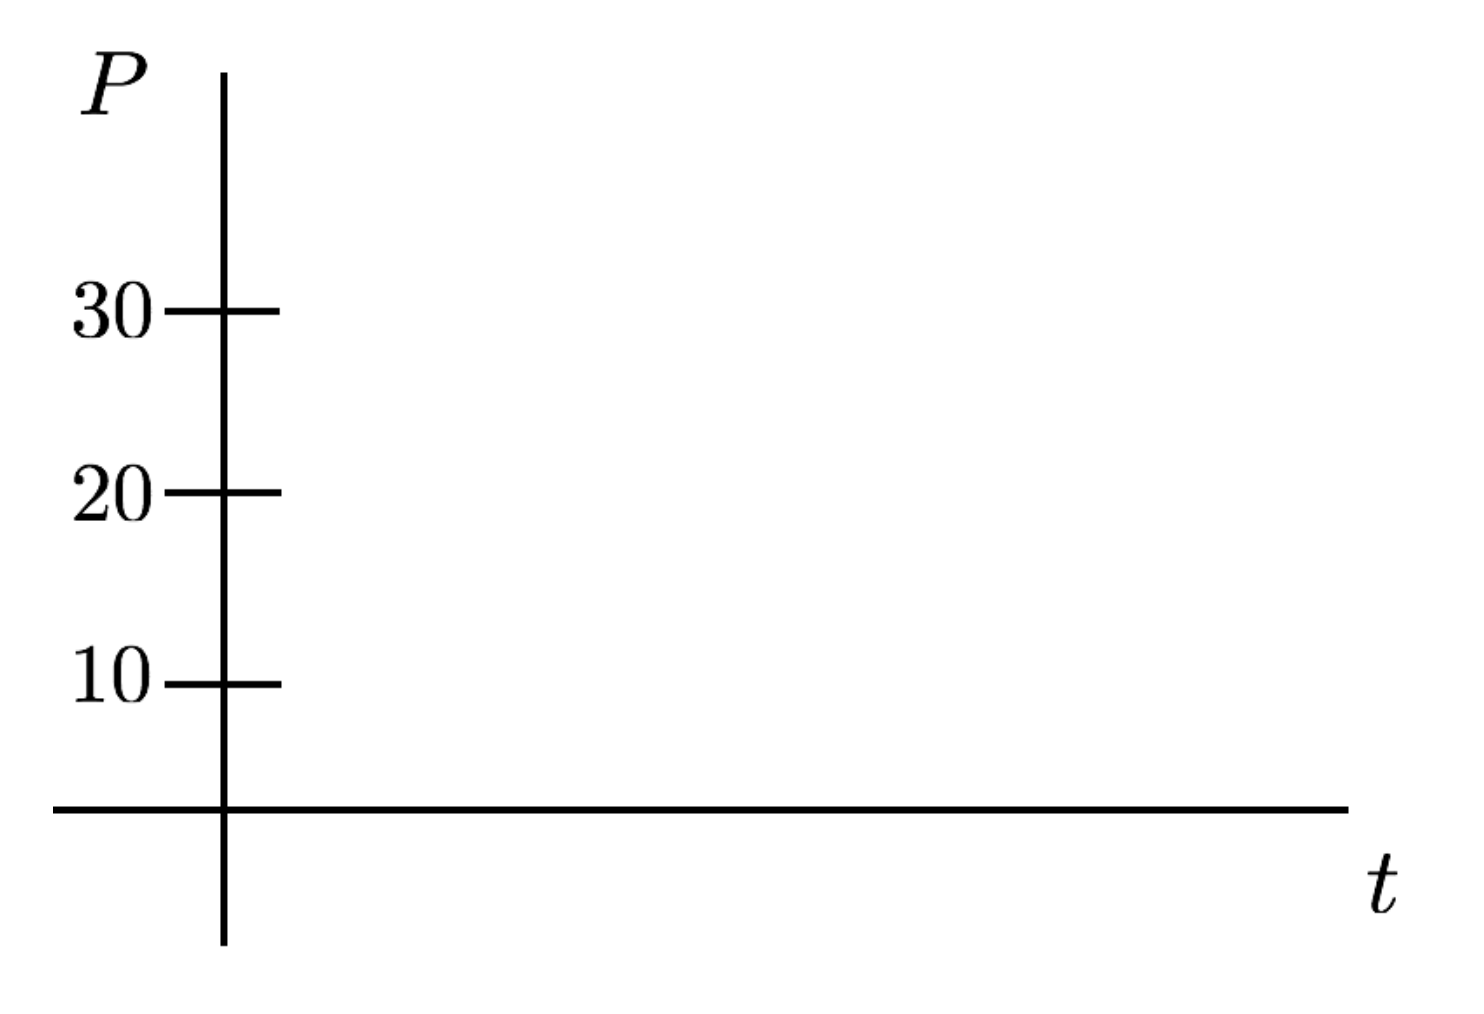
\includegraphics[width=3.5in]{01/01FishGraph.png}
\end{center}
\vspace{-.5in}
\begin{enumerate}
\item	For your graph starting with $P = 10$, how does the slope vary as time increases? Explain. \label{01problem2parta}
\vfill
\item	For a set $P$ value, say $P = 30$, how do the slopes vary across the three graphs you drew? \label{01problem2partb}
\vfill
\end{enumerate}
\item	This situation can also be modeled with a rate of change equation, $\frac{dP}{dt}=something$.  What should the ``something'' be? Should the rate of change be stated in terms of just $P$, just $t$, or both $P$ and $t$? Make a conjecture about the right hand side of the rate of change equation and provide reasons for your conjecture. \label{01problem3}
\end{enumerate}
\vfill

\clearpage
 
%%%%%%%%%%%%%%%%%
\pagebegin{What Exactly is a Differential Equation and What are Solutions?}

A {\bf differential equation} is an equation that relates an unknown function to its derivative(s). Suppose $y = y(t)$ is some unknown function, then a differential equation, would express the rate of change, $\frac{dy}{dt}$, in terms of $y$ and/or $t$. For example, all of the following are \textit{first order} differential equations.  

\[ \frac{dP}{dt}=kP,\qquad \frac{dy}{dt}=y+2t, \qquad \frac{dy}{dt}=t^2+5,\qquad \frac{dy}{dt}=\frac{6y-2}{ty}, \qquad \frac{dy}{dt}=\frac{y^2-1}{t^2+2t}
\]

 Given a differential equation for some unknown function, \textbf{solutions} to this rate of change equation are \textsl{functions} that satisfies the rate change equation. %A constant function that satisfies the differential equation is called an \textbf{equilibrium solution}.
\vs

One way to read the differential equation $\frac{dy}{dt} = y+2t$ aloud you would say, ``dee $y$ dee $t$ equals $y$ plus two times $t$.'' However, this does \textbf{not} relate to the \textsl{meaning} of the solution. 

\begin{enumerate}[resume]
\item \begin{enumerate}
\item Is the function $y=1+t$  a solution to the differential equation $\displaystyle\frac{dy}{dt}=\frac{y^2-1}{t^2+2t}$? How about the function $y=1+2t$?  How about $y = 1$?  Explain your reasoning. \label{01problem4parta} \vfill 

\item	Is the function $y=t^3+2t$    a solution to the differential equation $\displaystyle \frac{dy}{dt}=3y^2+2$?  Why or why not? \label{01problem4partb} \vfill

\end{enumerate}

\item	Figure out all the functions that satisfy the rate of change equation $\displaystyle \frac{dP}{dt}=0.3P$. \vfill

\item	Figure out all of the solutions to the differential equation $\displaystyle\frac{dy}{dt}=t^2+5$. \label{01problem6} \vfill
\end{enumerate}

 %sections 1.1-1.2 (half of original unit 1)
%UNIT 1: QUALITATIVE AND GRAPHICAL APPROACHES
% Is 2nd part of original 01.tex
%%%%%%%%%%%%%%%%%%%%%%%%%%%
%%%% Put the following at the top of each .tex file  %
\pagestyle{fancy}
\renewcommand{\theUnit}{1.2}
\ifthenelse{\isundefined{\UnitPageNumbers}}{}{\setcounter{page}{1}}
\rhead{Section \theUnit: Slope Fields}
\lhead{
\includegraphics[width=1.25cm]{IODE-logo.png}}
\rfoot{\mypage}
\lfoot{}
\cfoot{}
\fancypagestyle{firstfooter}{\footskip = 50pt}
\renewcommand{\footrulewidth}{.4pt}
%%%%%%%%%%%%%%%%%%%%%%%%%%%
\vspace*{-20pt} \thispagestyle{firstfooter}
\pagebegin{Slope Fields}

A \textbf{slope field} is a graphical representation of a rate of change equation. Given a rate of change equation, if we plug in particular values of $(t,y)$ then $\displaystyle\frac{dy}{dt}$ tells you the slope of the tangent vector to the solution at that point.
\vs
For example, consider the rate of change equation $\displaystyle\frac{dy}{dt}=y+2t$.  At the point (1, 3), the value of $\displaystyle\frac{dy}{dt}$ is 5. Thus, the slope field for this equation would show a vector at the point (1, 3) with slope 5.  A slope field depicts the exact slope of many such vectors, where we take each vector to be uniform length. Slope fields are useful because they provide a graphical approach for obtaining qualitatively correct graphs of the functions that satisfy a differential equation.

\begin{enumerate}
\item Below is a partially completed slope field for  $\displaystyle \frac{dP}{dt}=0.8P$. \label{01problem7}
\begin{enumerate}
\item	Plot many more tangent vectors to create a slope field. \label{01problem7parta}
\item	Use your slope field to sketch in qualitatively correct graphs of the solution functions that start at $P = 0, 0.5$, and $2$, respectively. Note: the value of $P$ at an initial time (typically $t = 0$) is called an \textbf{initial condition}. \label{01problem7partb}
\item	Recall that a solution to a differential equation is a function that satisfies the differential equation. Explain how the graph with initial condition $P(0) = 1$ can graphically be thought of as a solution to the differential equation when the differential equation is represented by its slope field. \label{01problem7partc}
\end{enumerate}

\begin{center}
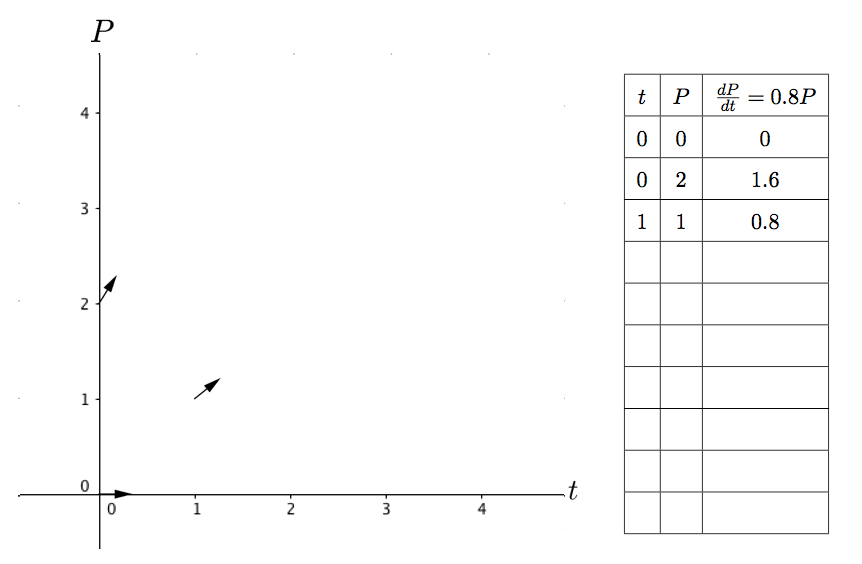
\includegraphics[width=6in]{02/02MyFirstSlopeFieldwithTable.png}
\end{center}

\clearpage

\item Below are seven rate of changes equations and three different slope fields. Without using technology, identify which differential equation is the best match for each slope field (thus you will have four rate of change equations left over). Explain your reasoning. \label{01problem8}
\[
\text{(i) } \frac{dy}{dt}=t-1 \quad \text{(ii) } \frac{dy}{dt}=1-y^2 \quad \text{(iii) } \frac{dy}{dt}=y^2-t^2 \quad \text{(iv) } \frac{dy}{dt}=1-y
\]
\[
\text{(v) } \frac{dy}{dt}=t^2-y^2 \quad \text{(vi) } \frac{dy}{dt}=1-t \quad \text{(vii) } \frac{dy}{dt}=9t^2-y^2
\]
\begin{enumerate*}
\item 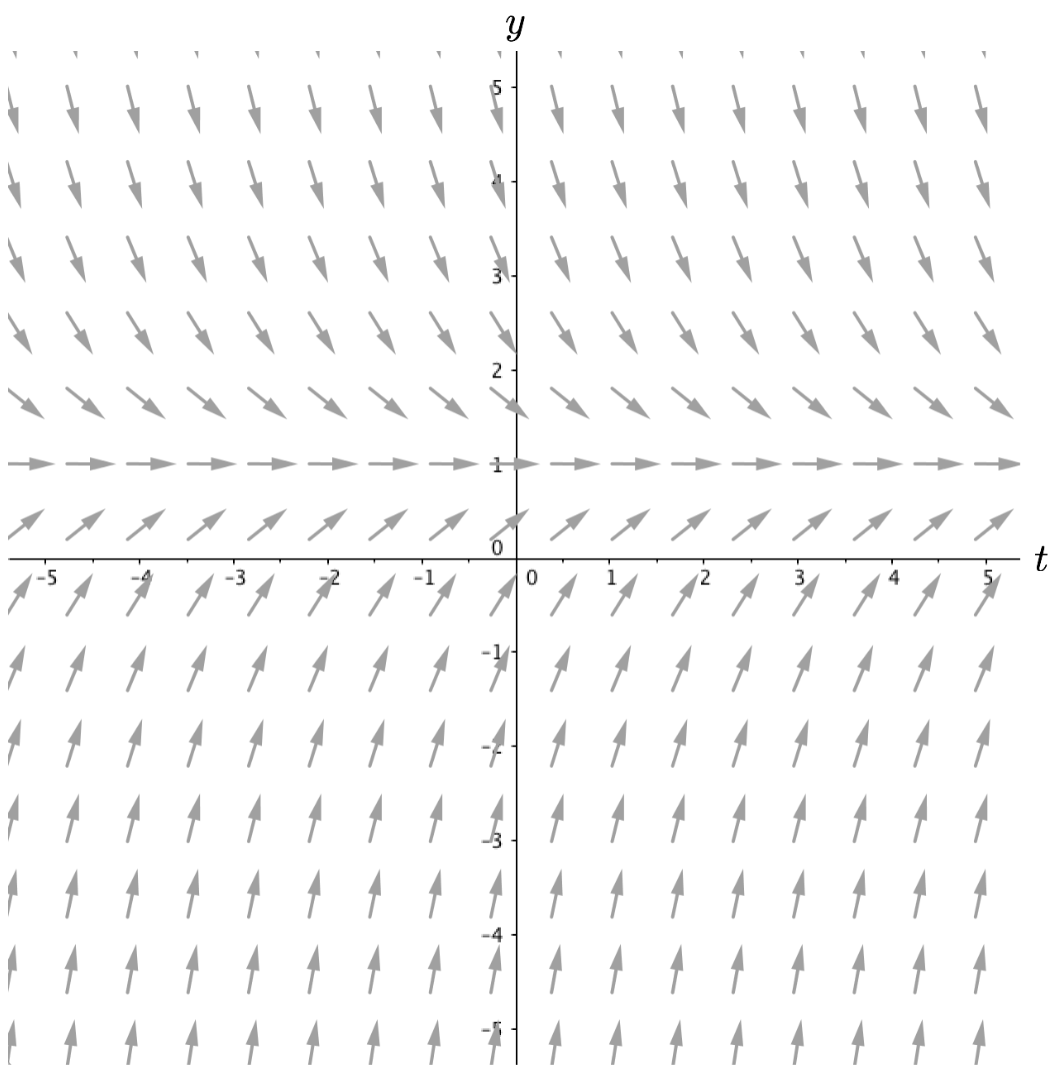
\includegraphics[width=2.75in]{02/02SlopeField1.png} \label{01problem8parta}
\item 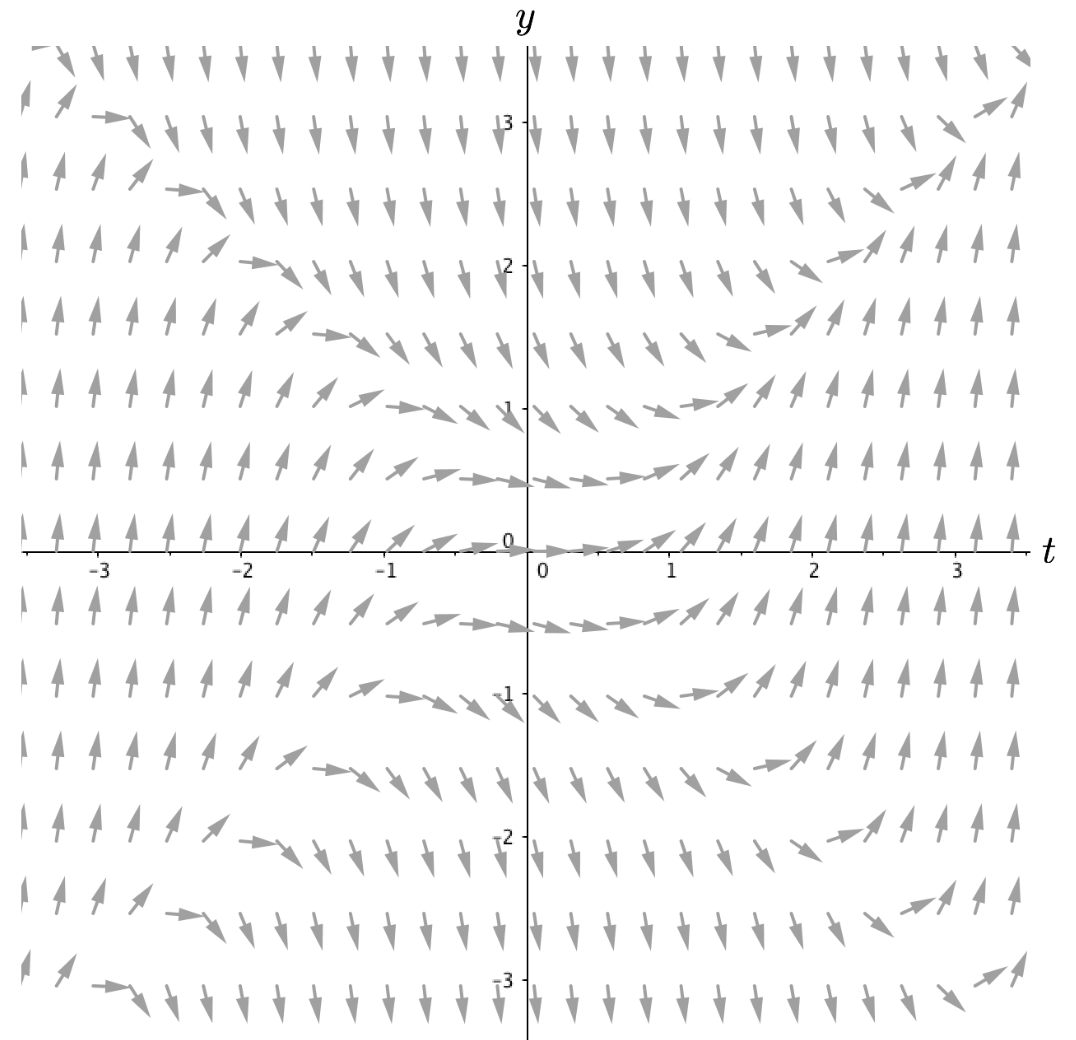
\includegraphics[width=2.75in]{02/02SlopeField2.png} \label{01problem8partb}
\end{enumerate*}

\begin{enumerate*}[resume]
\item 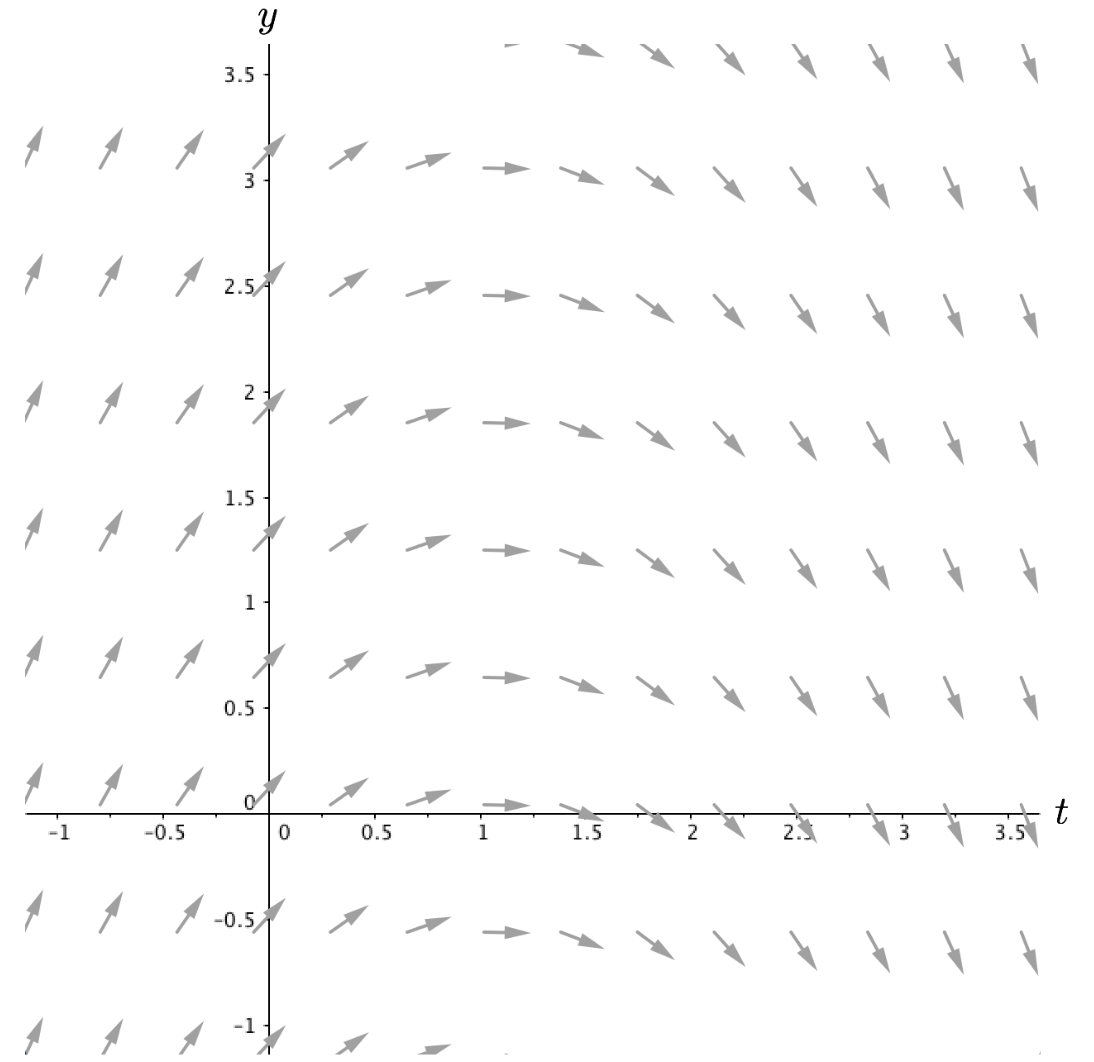
\includegraphics[width=2.75in]{02/02SlopeField3.png} \label{01problem8partc}
\end{enumerate*}
\vspace{0.1in}
\item For each of the slope fields in the previous problem, sketch in graphs of several different qualitatively correct solutions. \label{01problem9}
\vfill

\end{enumerate}


 %section 1.3 (half of original unit 1)
%UNIT 6: AUTONOMOUS DIFFERENTIAL EQUATIONS
%%%%%%%%%%%%%%%%%%%%%%%%%%%
%%%% Put the following at the top of each .tex file  %
\pagestyle{fancy}
\renewcommand{\theUnit}{C}
\ifthenelse{\isundefined{\UnitPageNumbers}}{}{\setcounter{page}{1}}
\rhead{Chap 1 Project \theUnit: Phase Line and Stability}
\lhead{
\includegraphics[width=1.25cm]{IODE-logo.png}}
\rfoot{\mypage}
\lfoot{}
\cfoot{}
\fancypagestyle{firstfooter}{\footskip = 50pt}
\renewcommand{\footrulewidth}{.4pt}
%%%%%%%%%%%%%%%%%%%%%%%%%%%
\vspace*{-20pt} \thispagestyle{firstfooter}
\pagebegin{Analyzing Autonomous DEs: Spotted Owls}

A group of biologists are making predictions about the spotted owl population in a forest in the Pacific Northwest.  The autonomous differential equation the scientist use to model the spotted owl population is $\displaystyle \frac{dP}{dt}=\frac{P}{2}\left(1-\frac{P}{5}\right)\left(\frac{P}{8}-1\right)$, where $P$ is in hundreds of owls and $t$ is in years. The problem is that the current number of owls is only approximately known.  
\begin{enumerate}
\item Suppose the scientists estimate that currently $P$ is about 5 (i.e. there are currently about 500 owls in the forest).  Since 5 is only an estimate, they make long-term predictions of the owl population for the initial conditions $P = 4.9$, $P = 5.0$, and $P = 5.1$. \textit{Without using a graphing calculator or other software}, determine the long-term predictions for these initial conditions based on the differential equation. Are they similar or different?  That is, will slightly different initial conditions yield only slightly different long-term predictions, or will they be radically different? Carry out a similar analysis if the current number of owls is somewhere around 8.\label{04problem1}
\vspace{4in}

\item Give a one dimensional representation, \textit{without words}, that would describe all solutions to the differential equation. \label{04problem2}

\clearpage
\item A \textbf{phase line} is the standard one-dimensional diagram that depicts the qualitative behavior of solutions to an autonomous differential equation. Label the dots and add arrows to the figure below to represent \textbf{all} solutions to the differential equation in Problem \ref{04problem1}. \label{04problem3} \\
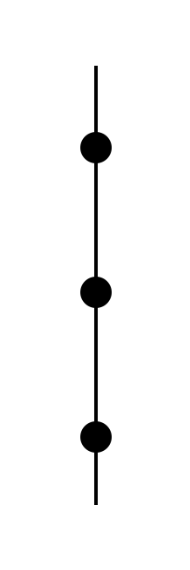
\includegraphics[width=1in]{04/04PhaseLine.png}

\item For the differential equation in problems \ref{04problem1}-\ref{04problem3} there are three equilibrium solutions. Recall that equilibrium solutions are constant functions that satisfy the differential equation. How do the other solution functions near each equilibrium solution behave in the long term? If you were to label each of these equilibrium solutions based on the way in which nearby solutions behave, what terms would you use and why? \label{04problem4} 

\end{enumerate}

\clearpage

\pagebegin{Phase Lines}

\begin{enumerate}[resume]
\item Dominique is working with the rate of change equation $\frac{dP}{dt}=0.2P$  and thinks about solutions in terms of whether they are increasing, decreasing, or remaining constant. She illustrates her thinking with the phase line shown below. 
\begin{center}
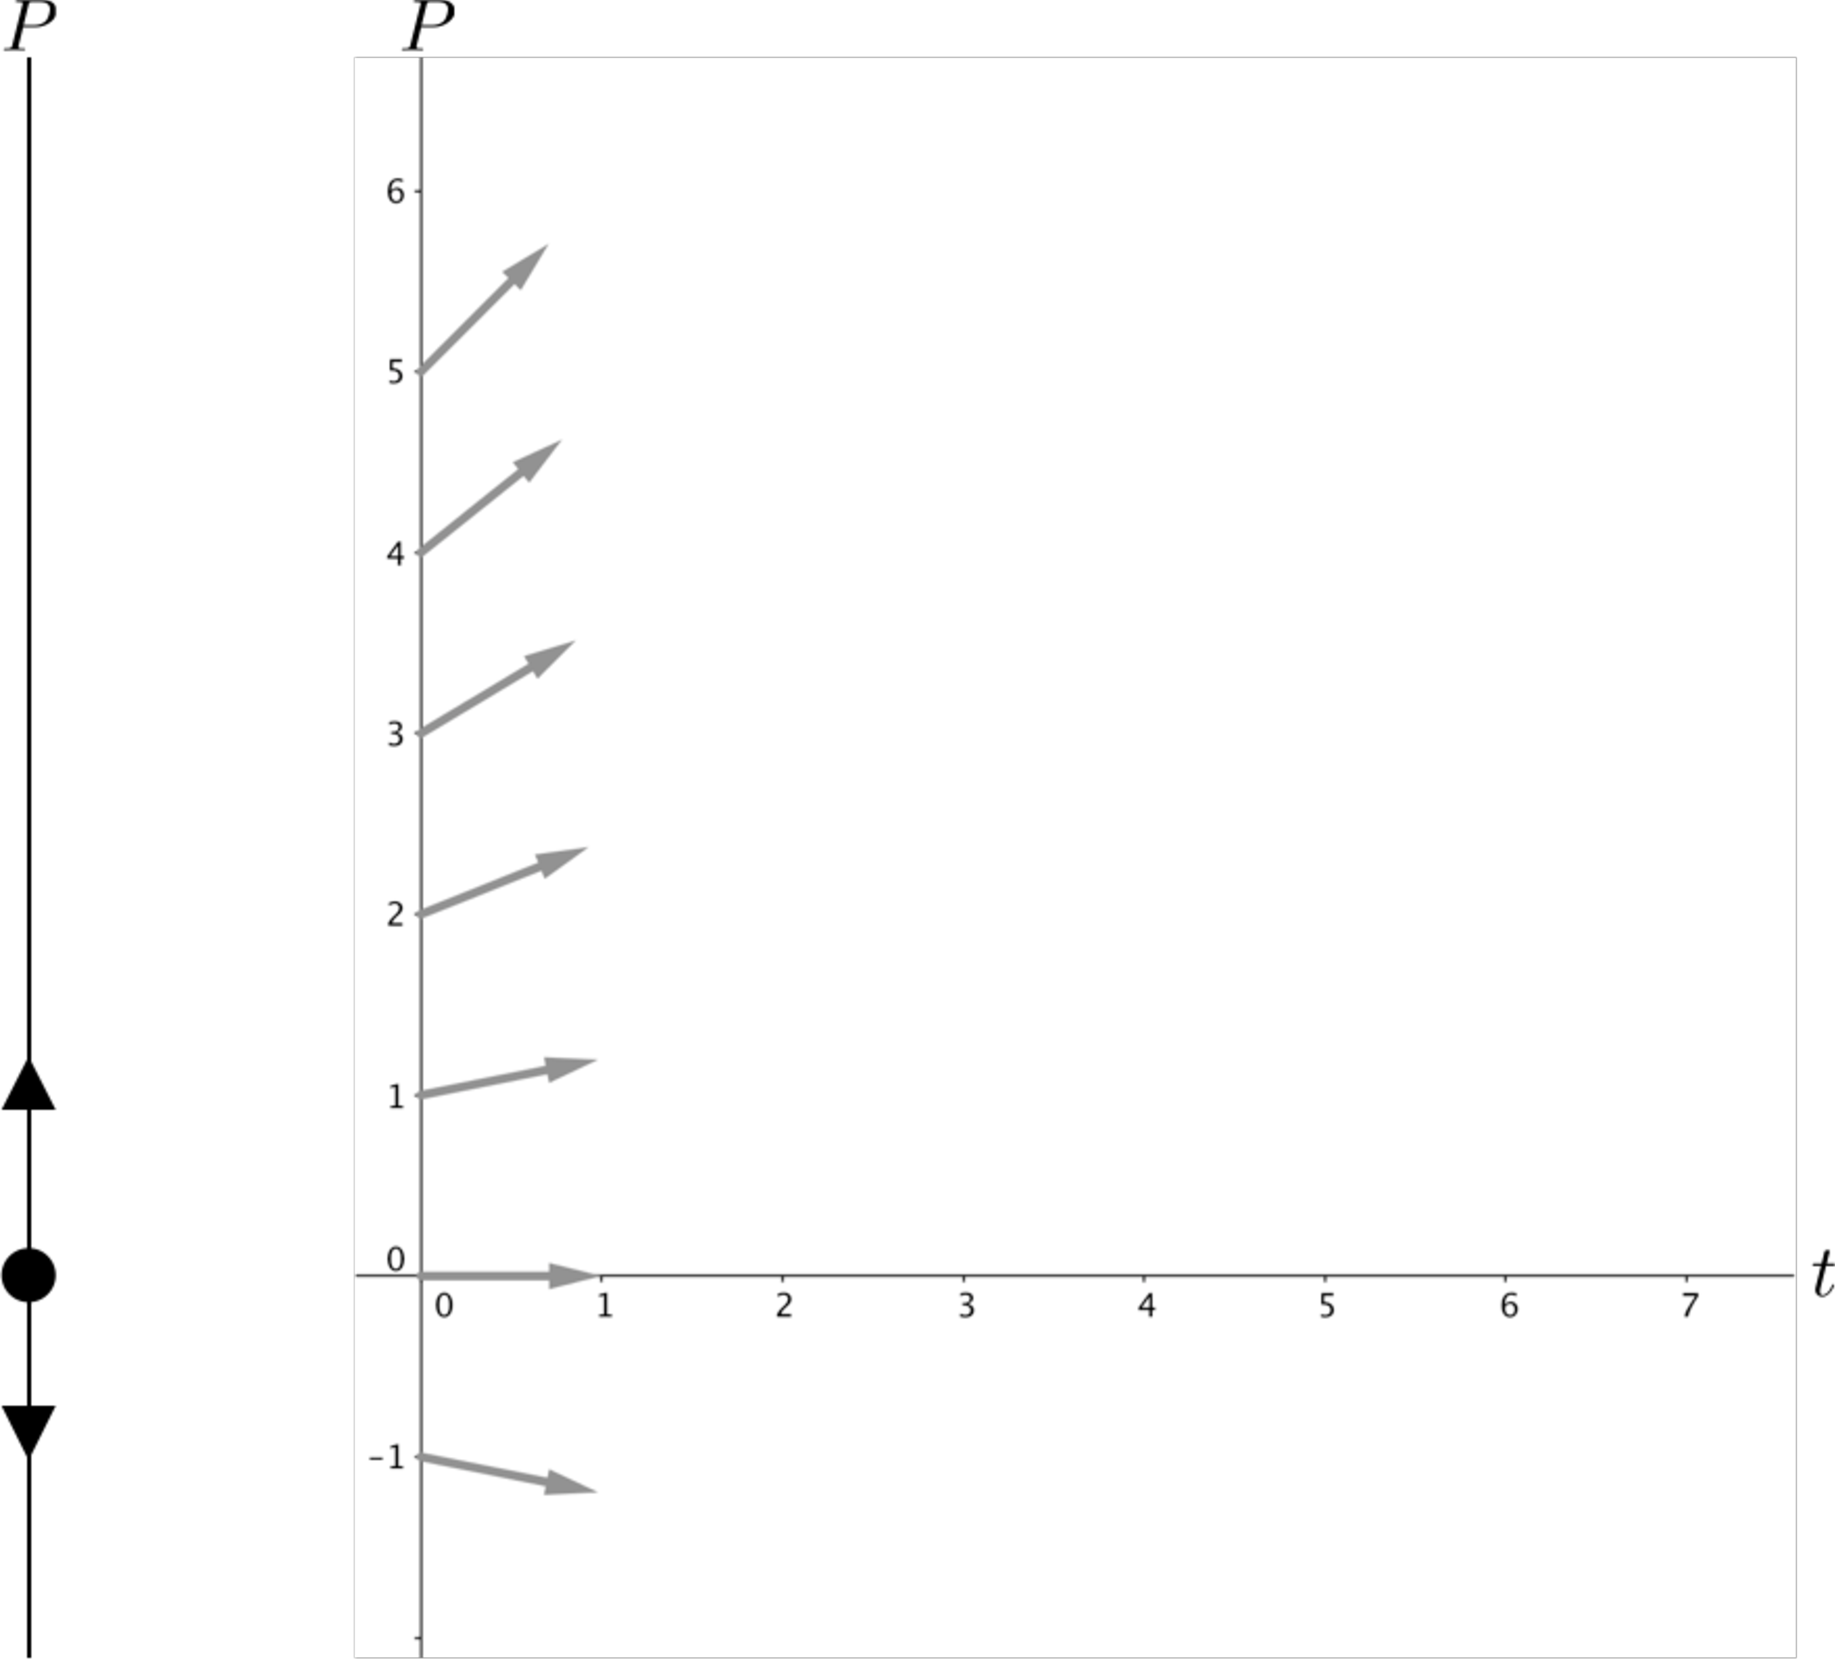
\includegraphics[width=6in]{04/04PhaseLineAndSomeVectors.pdf} \\
\end{center}
\clearpage
\begin{enumerate}
\item	Place your fingertip or other small item on the phase line at $P = 0$ and another fingertip or small item at $P = 0$ on the $P$ vs $t$ axes and imagine time moving forward. Explain, with reasons, what happens to your fingertips. \label{04problem5parta} \vfill

\item	Place your fingertip or other small item on the phase line at $P = 1$ and another fingertip or small item at $P = 1$ on the $P$ vs $t$ axes at (0,1) and imagine time moving forward. Explain, with reasons, what happens to your fingertips. \label{04problem5partb}   \vfill

\item	Place two fingertips or two small items on the phase line, one at $P = 1$ and the other at $P = 3$. What happens to your fingertips as time moves forward? How do your ideas relate to the corresponding $P$ versus $t$ graphs? \label{04problem5partc}  \vfill

\item	Explain how a person could think about the phase line as a one-dimensional projection of all of the two-dimensional $P(t)$ graphs of solutions. \label{04problem5partd} \vfill

\end{enumerate}
\end{enumerate}
\clearpage

%%%%%%%%%%%%%%%%%%%%%%%%%%%%%%%%%%%%%%%%%%%%%%%%%%%%%%%%%%%%%%%%%%%%%%%%%%%%%%%%%%%%%%%%%%
\pagebegin{Homework Set 4}

\begin{enumerate}
\item For an autonomous differential equations, it is possible to view all of the solution function graphs in terms of ``prototypical'' graphs. A prototypical solution graph represents an infinite number of other solution graphs. For example, in part (i) below one can view the entire family of functions that solve the differential equation in terms of two different prototypical solution graphs separated by an equilibrium solution: one prototypical solution graph is above the $t$-axis and one is below the $t$-axis. Each is prototypical because it can stand for all other solution graphs (in its respective region) through horizontal translation. Recall the ``Making Connections'' section of Unit 3. \label{04HWproblem1}
\begin{hnumerate}
\hitem    $\displaystyle\frac{dy}{dt}=-y$    \hitem $\displaystyle\frac{dy}{dt}=2y\left(1-\frac{y}{2}\right)$        \hitem $\displaystyle\frac{dy}{dt}=2y\left(1-\frac{y}{2}\right)+3$        \hitem   $\displaystyle\frac{dy}{dt}=y^2$ \end{hnumerate}
\begin{enumerate}
\item For each differential equation above, draw a phase line and representative graphs of solutions. \label{04HWproblem1parta}
\item For each differential equation above, explain how your response to number \ref{04HWproblem1parta} can be interpreted in terms of prototypical solutions separated by equilibrium solutions. \label{04HWproblem1partb} 
\end{enumerate}

\item For each of the following slope fields, create a differential equation whose slope field would be similar to the one given. Give reasons for why you created the differential equation as you did. You may create whatever scale on the axes that you want. \label{04HWproblem2} \\
\begin{enumerate*}
\item 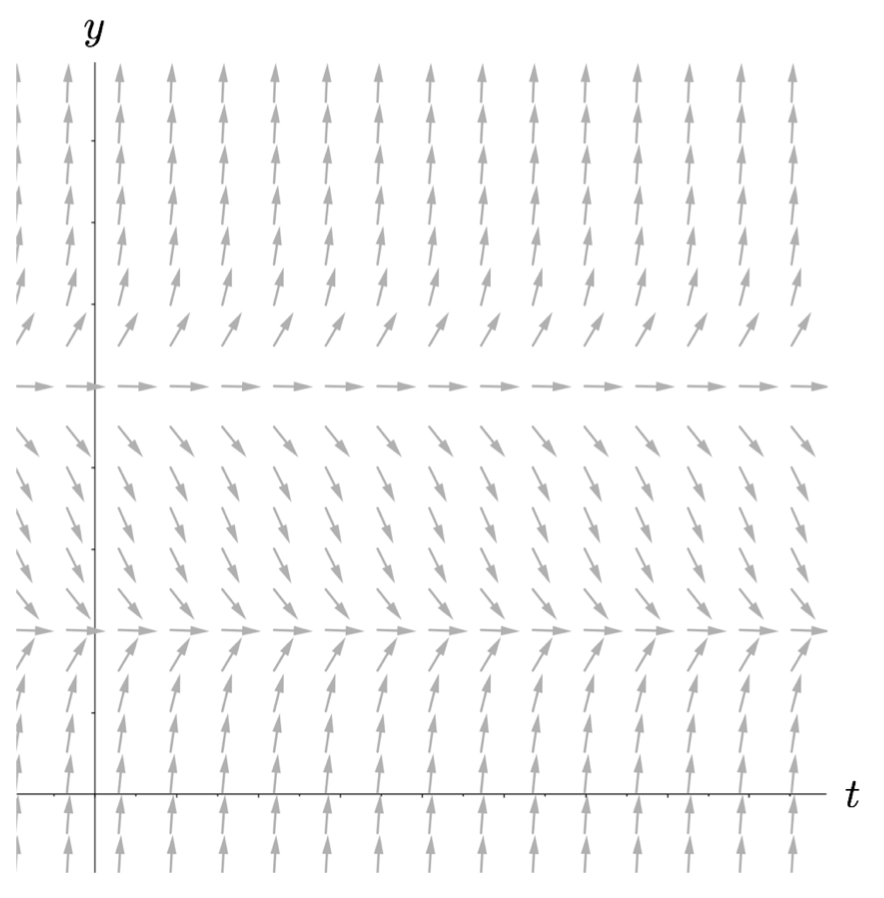
\includegraphics[width=3in]{04/04HWSlopeFieldA.png}
\item 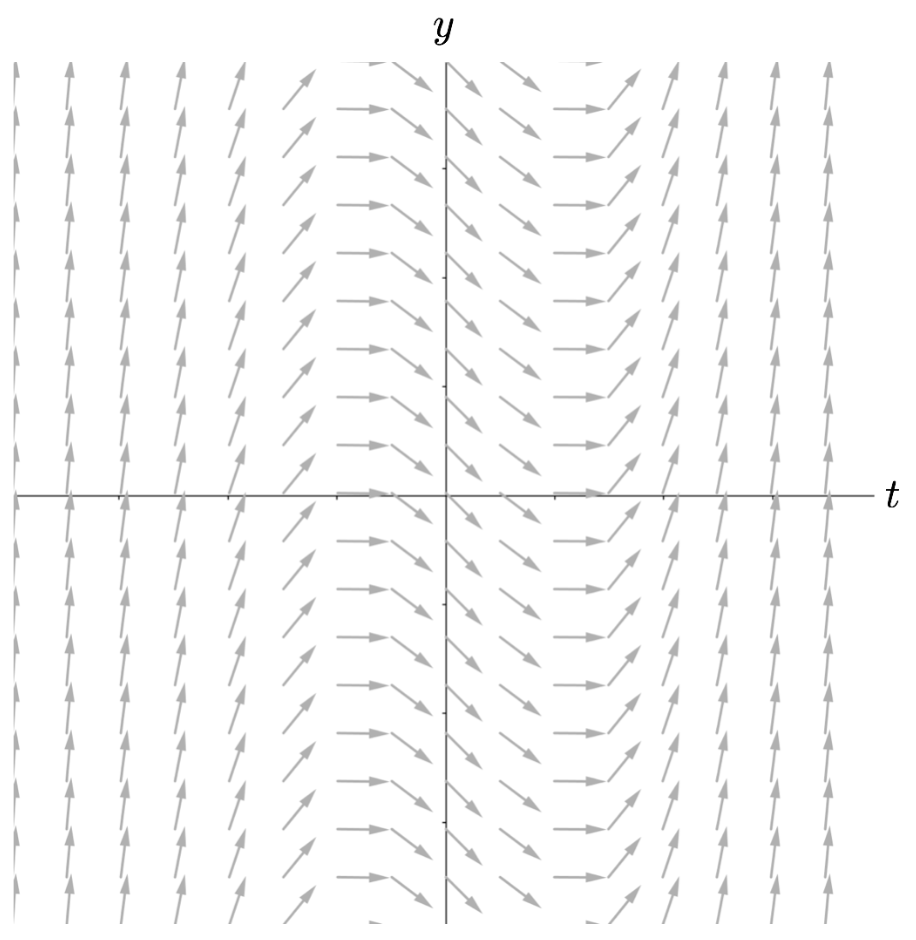
\includegraphics[width=3in]{04/04HWSlopeFieldB.png}
\item 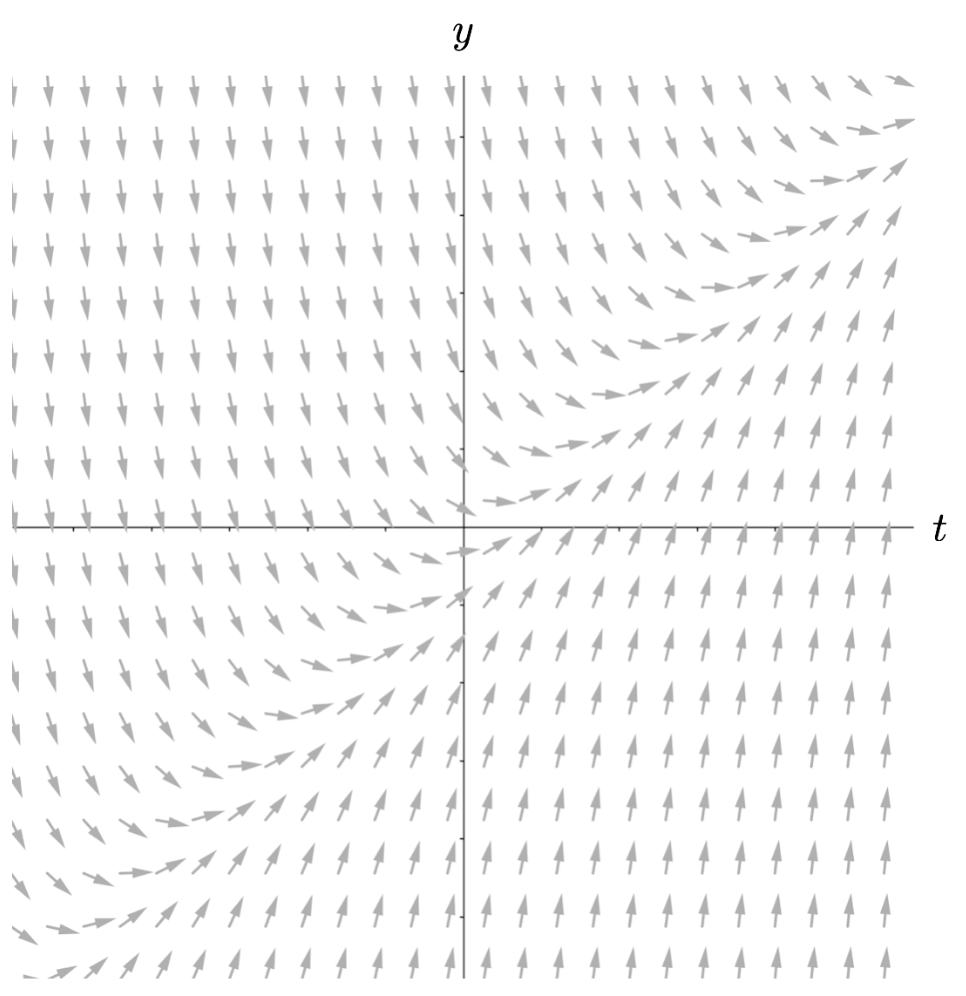
\includegraphics[width=3in]{04/04HWSlopeFieldC.png}
\item 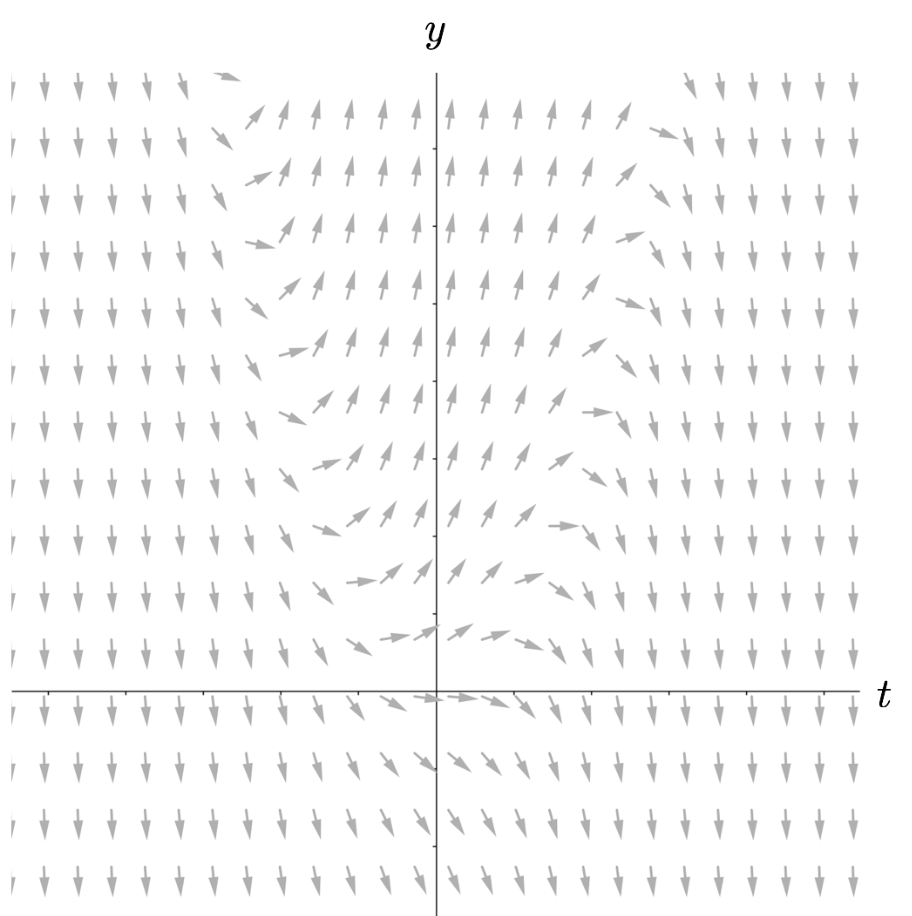
\includegraphics[width=3in]{04/04HWSlopeFieldD.png}
\end{enumerate*}

\item For each part below, create a continuous, autonomous differential equation that has the stated properties (if possible). Explain how you created each differential equation and include all graphs or diagrams you used and how you used them. If it is not possible to come up with a differential equation with the stated properties, provide a justification for why it cannot be done. \label{04HWproblem3}

\begin{enumerate}
\item Exactly three constant solution functions, two repellers and one attractor.
\item	Exactly two constant solution functions, one a repeller and one a node.
\item	Exactly two constant solution functions, both attractors.
\end{enumerate}

\item For each part below, create an autonomous differential equation that satisfies the stated criteria \label{04HWproblem4}
\begin{enumerate}
\item	$y(t)=0$ and $y(t) = -4$ are the only constant solution functions
\item $y(t)=e^{-t+1}$ is a solution
\item $y(t)=e^{2t-5}$	is a solution
\item $y(t)=10e^{0.3t}$ is a solution
\item $y(t)=1-e^{-t}$ and $y(t)=1+e^{-t}$ are solutions
\end{enumerate}

\item For a phase line to be a meaningful tool, explain why it is essential for the differential equation to be autonomous. \label{04HWproblem5}

\item In class you and your classmates continue to develop creative and effective ways of thinking about particular ideas or problems. Discuss at least one idea or way of thinking about a particular problem that has been discussed in class (either in whole class discussion or in small group) that was particularly helpful for enlarging your own thinking and/or that you disagreed with and had a different way of thinking about the idea or problem. \label{04HWproblem6}

\end{enumerate}
 %section Project C (original unit 6)
%UNIT 3: AN ANALYTIC APPROACH
%%%%%%%%%%%%%%%%%%%%%%%%%%%
%%%% Put the following at the top of each .tex file  %
\pagestyle{fancy}
\renewcommand{\theUnit}{3}
\ifthenelse{\isundefined{\UnitPageNumbers}}{}{\setcounter{page}{1}}
\rhead{Unit \theUnit: An Analytic Approach}
\lhead{
\includegraphics[width=1.25cm]{IODE-logo.png}}
\rfoot{\mypage}
\lfoot{}
\cfoot{}
\fancypagestyle{firstfooter}{\footskip = 50pt}
\renewcommand{\footrulewidth}{.4pt}
%%%%%%%%%%%%%%%%%%%%%%%%%%%
\vspace*{-20pt} \thispagestyle{firstfooter}
\pagebegin{Comparing Predictions}

Jerry and Tom are using the differential equation $\displaystyle\frac{dP}{dt} = 0.2P$ to make predictions about the number of a particular species of fish in Lake Michigan. They know that the initial population $P$ is 2 at time $t = 0$ (as before, think of 2 as scaled for say, 2,000 or 20,000).
 \vs
Although Jerry and Tom have the same goal (to obtain predictions for future fish population), they have different approaches to achieve this goal. 

\begin{itemize}
\item	Tom's approach is to create a graph of the number of fish versus time by connecting slope vectors tip-to-tail, where the rate of change is constant over some time interval, for example $\Delta t=0.5$. 
\item Jerry's approach is to create a graph of the number of fish versus time by using a continuously changing rate of change. 

\end{itemize}
\begin{enumerate}

\item Sketch Tom and Jerry's approaches below. Will these two approaches result in the same predictions for the number of fish in, say, $2.5$ years? If yes, why? If not, how and why will the graphs of their approaches be different?\label{03problem1}
\begin{center}
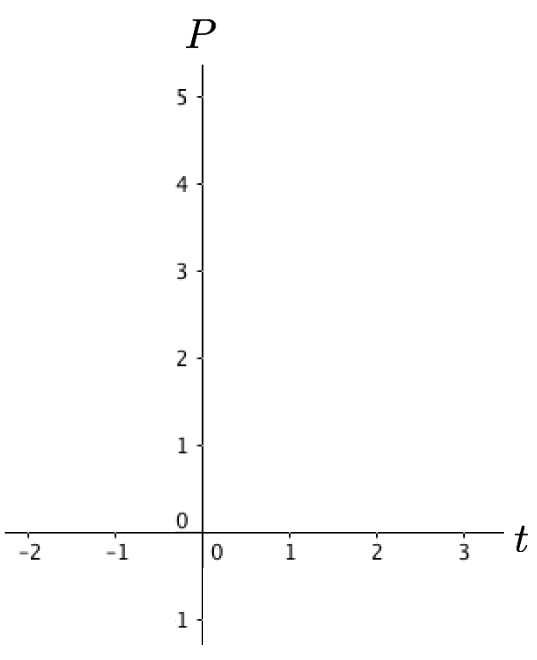
\includegraphics[width=3in]{03/03TomJerry.png}
\end{center}
\end{enumerate}
\clearpage

%%%%%%%%%%%%%%%%%%%%%%
\pagebegin{Separation of Variables}

\begin{enumerate}[resume]
\item	\textbf{Finding the exact solution}. Jerry's approach involves using a continuously changing rate of change, which corresponds to finding an ``exact solution.'' \label{03problem2}
\begin{enumerate}

\item	Why do you think the phrase ``exact solution'' is used to describe the result of Jerry's approach? Explain why it is appropriate to describe the result of Tom's approach as an ``approximate solution''. \label{03problem2parta}

\vfill
\item Use the chain rule to write down, symbolically, the derivative with respect to $t$ of $\ln (P)$, where $P$ is shorthand for $P(t)$. \label{03problem2partb}
\end{enumerate}
\vfill

\clearpage

Next you will learn a technique for finding the exact solution corresponding to Jerry's approach. We begin by considering the chain rule.

\begin{enumerate}[resume]
\item	 The following is a method to find the analytic solution to $\displaystyle\frac{dP}{dt}= 0.2P$. For now assume that $P > 0$. This assumption corresponds to the population growth context and it will make the algebra easier and hence the underlying idea clearer.  \label{03problem2partc}
 
\end{enumerate}

\begin{center} \renewcommand{\arraystretch}{1.5}
\newcolumntype{V}{>{\centering\arraybackslash} m{.5\linewidth} }
\begin{tabular}{|p{2in}|V|}
\hline

Divide both sides of \newline $\frac{dP}{dt}=0.2P$ by $P$ &
{} \\
{} & {} \\
\hline

Replace $\frac{1}{P}\frac{dP}{dt}$ with $\left[ \ln(P)\right]'$ & 
{} \\
{} & {} \\
\hline
	 
Write integrals with respect to $t$ on both sides & 
\\{} & {} \\ 
\hline
	 
Apply the Fundamental Theorem of Calculus to integrate both sides & 
\\{} & {} \\
\hline	 

Solve for $P$ (and remember that $P$ is actually a function, $P(t)$) & 
\\{} & {} \\
\hline

Show that $P$ can be written as $P(t) = ke^{0.2t}$ & 
\\{} & {} \\
{} & {} \\
\hline
\end{tabular} \end{center}

The end result, $\displaystyle P(t)=ke^{0.2t}$ is called the \textbf{general solution} because it represents all possible functions that satisfy the differential equation. We can use the general solution to find any \textbf{particular solution}, which is a solution that corresponds to a given initial condition.

\item	Use the same technique to find the general solution to $\displaystyle\frac{dy}{dt}=\frac{t}{3y^2}$. The first step is done for you. \label{03problem3}
\vs
$\displaystyle 3y^2\frac{dy}{dt}=t$
\vfill

\clearpage

\item In practice, we often circumvent explicit use of the chain rule and instead use a shortcut to more efficiently find the general solution. The shortcut involves treating the derivative $\frac{dP}{dt}$ as a ratio and ``separating'' the $dP$ and $dt$. In the table below, follow the instructions to see how the shortcut works, using again the equation $\displaystyle\frac{dP}{dt} = 0.2P$. (See \href{http://kevinboone.net/separation_variables.html}{\underline{http://kevinboone.net/separation\textunderscore variables.html}}) for a nice explanation of the shortcut). \label{03problem4}
\vs

\begin{center}\renewcommand{\arraystretch}{1.5}
\newcolumntype{V}{>{\centering\arraybackslash} m{.5\linewidth} }
\begin{tabular}{|p{2.5in}|V|}
\hline
`Separate' the $dP$ from the $dt$ so that $dP$ and $P$ are on the same side. (If there are $t$'s in the equation they must go on the same side as $dt$.)
	  &
{} \\\hline

Integrate both sides of the equation (one side with respect to $P$, the other with respect to $t$)	  &
{} \\\hline

Continue as before to arrive at a solution of the form $P(t)=\underline{\hskip1cm}$	 	  &
{} \\
{} & {} \\
{} & {} \\
{} & {} \\
{} & {} \\
{} & {} \\
{} & {} \\
{} & {} \\ \hline
\end{tabular}
\end{center}

\item	Use the shortcut to find the general solution to  $\displaystyle \frac{dy}{dt}=\frac{t}{3y^2}$. \label{03problem5}
\vfill

\clearpage

\item	A differential equation together with an initial condition is called an \textbf{Initial Value Problem} (IVP). To solve an IVP one first must find the general solution and then use the initial condition to find the particular solution corresponding to the initial condition. \label{03problem6} \\ Solve the following IVP:    
\[ \frac{dy}{dt}=\frac{t}{y}\hspace{0.5in} y(2)=-1\]
\vfill

\begin{enumerate}
\item	 For what values of $t$ is your solution valid? Why? \label{03problem6parta} 
\vskip1cm

\item Check to see that your {particular} solution ``fits'' the differential equation by substituting the solution and its derivative into the original differential equation. \label{03problem6partb} 
\vfill

\item	Use the GeoGebra applet, \href{https://ggbm.at/SbHk2n4H}{\underline{https://ggbm.at/SbHk2n4H}}, to check to see that your specific solution ``fits'' the differential equation by plotting the slope field and then plotting the graph of the solution on top of the slope field. Explain how this relates to Jerry's approach. \label{03problem6partc}

\vspace{-.25in}\hspace{-.75in}
\includegraphics[width=0.5in]{03/03IVPQR.png}
\vfill

\item Even though $\displaystyle\frac{dy}{dt}$ is undefined when $y=0$, the solution function can be defined such that $y(2)=0$.  What should the graph of this solution look like in the slope field? \label{03problem6partd} 
\vfill
\end{enumerate}

\end{enumerate}

\clearpage

%%%%%%%%%%%%%%%%%%
\pagebegin{Making Connections}

\begin{enumerate}[resume]
\item For the first slope field for $\frac{dL}{dt} = 0.5(1 - L)$ on the following page,\label{03problem7}
\begin{enumerate}

\item	Using Jerry's approach, sketch as accurately as possible a graph of the solution with initial condition $L(0) = 1/3$. \label{03problem7parta}
\item	Make a copy of this sketch on a transparency. \label{03problem7partb}
\item	If you wanted to obtain the graph of the solution with initial condition $L(0) = 1/2$, how, if at all, might you move the copy of your graph with initial value 1/3 so that it is now a graph of the solution with initial value 1/2? What feature of the differential equation justifies your approach? \label{03problem7partc}
\item	Find the general solution for $\displaystyle\frac{dL}{dt} = 0.5(1�-L)$ and explain how your results from part \ref{03problem7partc} can be understood from the general solution.\label{03problem7partd}
\vfill	

\end{enumerate}
\item	For the second slope field for $\frac{dh}{dt} = -t + 1$ on the following page,\label{03problem8}
\begin{enumerate}
\item	Using Jerry's approach, sketch as accurately as possible a graph of the solution with initial condition $h(0) = 1/2$. \label{03problem8parta}
\item	Make a copy of this sketch on a transparency. \label{03problem8partb}
\item	If you wanted to obtain the graph of the solution with initial condition $h(0) = 1$, how, if at all, might you move the copy of your graph with initial value $1/2$ so that it is now a graph of the solution with initial value 1? Explain your idea and provide reasons for why your idea makes sense. \label{03problem8partc}
\item	Find the general solution for $\frac{dh}{dt} = -t + 1$ and explain how your results from part \ref{03problem8partc} can be understood from the general solution. \label{03problem8partd} \vfill
\end{enumerate}

\item  Give an example of a differential equation where neither of your ideas from \ref{03problem7partc} and \ref{03problem8partc} will work and provide reasons for your response.\label{03problem9}\vfill
\end{enumerate}

\clearpage

\begin{center}
\textbf{Slope Field} for $\displaystyle\frac{dL}{dt} = 0.5(1 - L)$

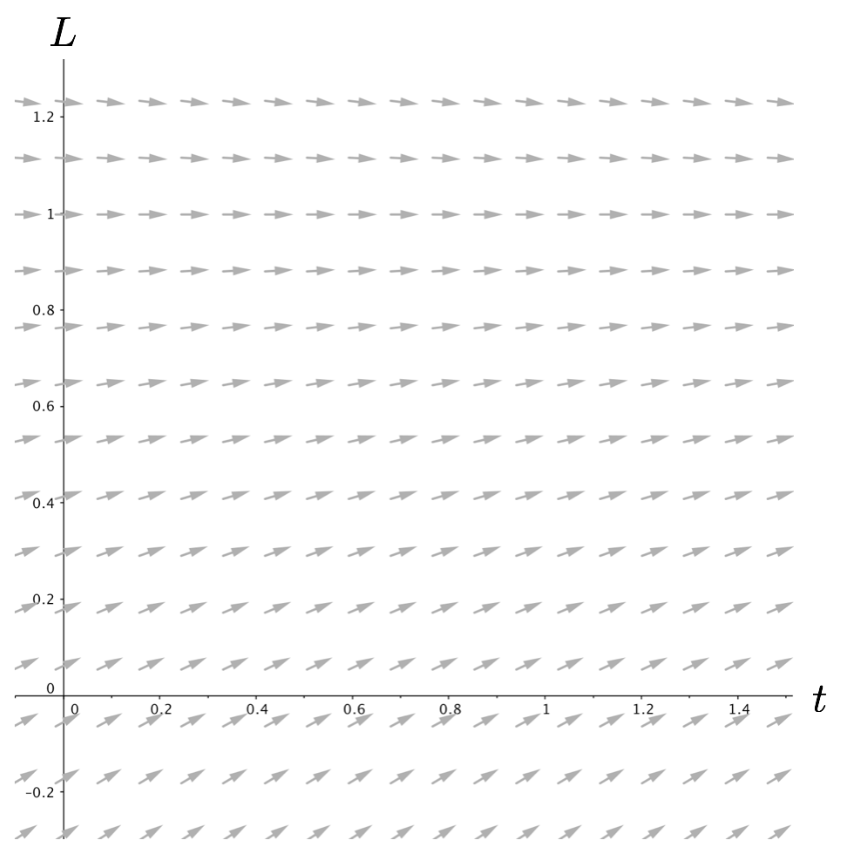
\includegraphics[width=4in]{03/03SlopeField1.png}

\vspace{.5cm}
\textbf{Slope Field} for $\displaystyle\frac{dh}{dt} = -t + 1$

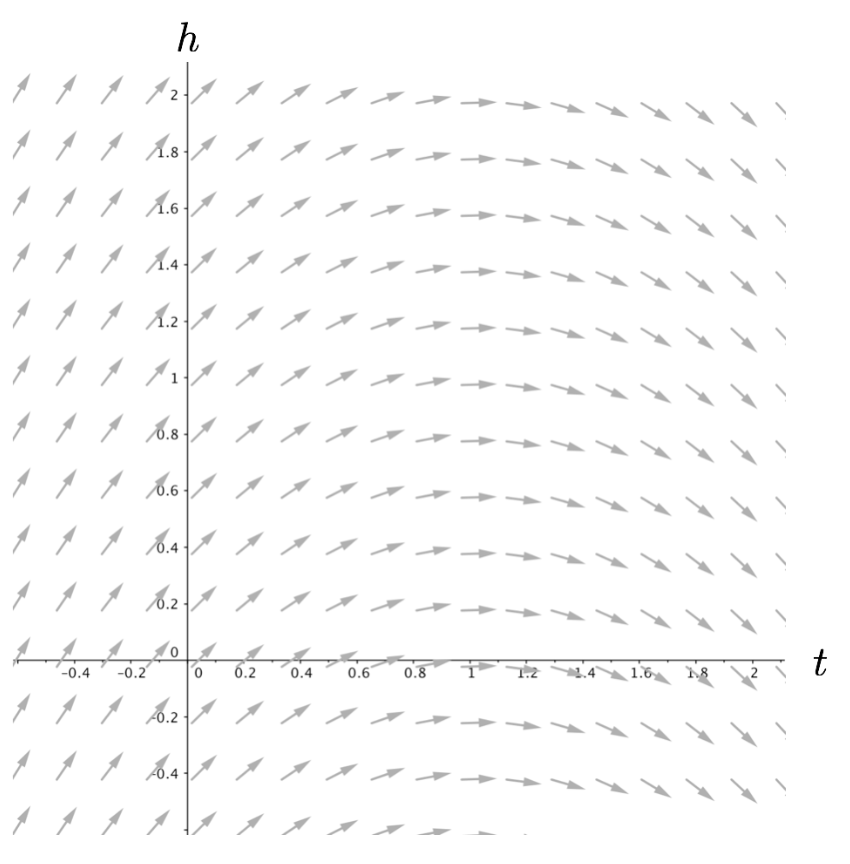
\includegraphics[width=4in]{03/03SlopeField2.png}\\
\end{center}

\clearpage

%%%%%%%%%%%%%%%%%%%%%%%%%%%%%%%%%%%%%%
\pagebegin{Homework Set 3}
\begin{enumerate}

\item When you solve an equation such as $x^2-3=1$ , you get two numbers $x=2$ and $x= -2$.  When you solve a differential equation, what do you get? \label{03HWproblem1}

\item Find the general solution to the following differential equations. \label{03HWproblem2}

\begin{enumerate}
\item $\displaystyle \frac{dy}{dt}=t^4y$
\item $\displaystyle \frac{dy}{dt}=2y+1$
\item $\displaystyle \frac{dy}{dt}=t\sqrt[3]{y}$
\item $\displaystyle \frac{dy}{dt}=\frac{t}{y+1}$
 \item $\displaystyle 2\frac{dy}{dx}=xy(x+1)$
\end{enumerate}
	 
\item	Find the particular solution to the following initial value problems. \label{03HWproblem3}
\begin{enumerate}
\item $\displaystyle \frac{dy}{dt}=\frac{-t}{y}, \qquad y(0)=4$
\item $\displaystyle \frac{dy}{dt}=-\sqrt[3]{y}, \qquad y(0)=27$
\item $\displaystyle \frac{dy}{dx}=\frac{x(y-2)}{x^2+4}, \qquad y(1)=5$
\end{enumerate}
	 
\item	Develop a differential equation where $y(t) = 6$ is a solution function but $y(t) = 8$ is not a solution function. Explain why your differential equation meets both of these criteria. \label{03HWproblem4}

\item Denise has created the following graph to go along with the rate of change equation $\frac{dP}{dt}=0.2P$. \label{03HWproblem5}
\begin{center}
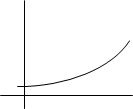
\includegraphics[]{03/03Denise.png}
\end{center}
What is this a graph of? Label the axes and explain your reasoning.

\clearpage

\item Cornelia is working with the differential equation $\displaystyle\frac{dy}{dt}= y - t$.  She has no method like separation of variables to use but still needs to a way to figure out which, if any, of the following functions are solutions to $\displaystyle\frac{dy}{dt}= y - t$. \label{03HWproblem6}
\[
\text{(i) }y(t)= t + 2 \hspace{.75in} \text{(ii) }y(t)= e^t-1 \hspace{.75in} \text{(iii) }y(t) = e^t  + t + 1 \hspace{.75in} \text{(iv) }y(t) = t
\]
  
\begin{enumerate}
\item Read the differential equation $\displaystyle\frac{dy}{dt}= y - t$ with {\em meaning}. Write down exactly how you would read the equation with meaning. Recall {\em reading with meaning} was discussed in Unit 1.
\item	Explain how Cornelia can use a slope field to determine which, if any, of these functions are solutions to the differential equation, $\displaystyle\frac{dy}{dt}= y - t$. 
\item	Use what it means to be a solution to a differential equation to determine which, if any, of these functions are solutions to $\displaystyle\frac{dy}{dt}= y - t$.  Show all work.
\end{enumerate}

\end{enumerate}

 %section 1.4 (original unit 2)
%UNIT 5: UNIQUENESS OF SOLUTIONS	
%%%%%%%%%%%%%%%%%%%%%%%%%%%
%%%% Put the following at the top of each .tex file  %
\pagestyle{fancy}
\renewcommand{\theUnit}{5}
\ifthenelse{\isundefined{\UnitPageNumbers}}{}{\setcounter{page}{1}}
\rhead{Unit \theUnit: Uniqueness of Solutions}
\lhead{
\includegraphics[width=1.25cm]{IODE-logo.png}}
\rfoot{\mypage}
\lfoot{}
\cfoot{}
\fancypagestyle{firstfooter}{\footskip = 50pt}
\renewcommand{\footrulewidth}{.4pt}
%%%%%%%%%%%%%%%%%%%%%%%%%%%
\vspace*{-20pt} \thispagestyle{firstfooter}
\pagebegin{Proposed Paths of Descent}

A group of scientists at the Federal Aviation Association has come up with the following two different rate of change equations to predict the height of a helicopter as it nears the ground: 
\[ \frac{dh}{dt}=-h \qquad \text{ and } \qquad \frac{dh}{dt}=-h^{\frac{1}{3}}\]
 
For both rate of change equations $h$ is in feet and $t$ is in minutes. The scientists, of course, want their models to predict that a helicopter actually lands - but do either or both of the proposed models predict this? 
\begin{enumerate}
\item Getting familiar with the differential equations: \label{05problem1}

\begin{enumerate}
\item Just by examining the rate of change equations, what can you say about the height of the helicopter as predicted by $\displaystyle\frac{dh}{dt}=-h$  and by $\displaystyle\frac{dh}{dt}=-h^{\frac{1}{3}}$? More specifically, as $h$ approaches zero, what can you say about $\displaystyle\frac{dh}{dt}$ and what does that imply about whether the model predicts that the helicopter lands? \label{05problem1parta}
\vfill

\item Sketch your best guess for a height versus time solution graph for each rate of change equation. \label{05problem1partb}
\end{enumerate}
\vfill

\item	\label{05problem2}
\begin{enumerate}
\item What do each of the proposed rate of change equations say about the solution to the differential equation if the helicopter is already on the ground? Explain and sketch a corresponding graph of height versus time on the same set of axes from part \ref{05problem1partb}. \label{05problem2parta}
\vfill

\item Interpret the initial condition $h(0) = 0$, and explain why $h(t) = 0$ should be a solution to each differential equation under this initial condition. \label{05problem2partb}
\vfill
\end{enumerate}

\clearpage

\item Use the Geogebra applet, \href{https://ggbm.at/dJsACfAN}{\underline{https://ggbm.at/dJsACfAN}}, to investigate the slope fields. What do the slope fields suggest about whether the model predicts if the helicopters will land?  How do the slope fields compare with your sketches from part \ref{05problem1partb}? \label{05problem3}

\vspace{-.05in}\hspace{-.5in}
\includegraphics[width=0.5in]{05/05ProposedPathsQR.png}
\vfill

\item Solve the following initial value problems: \label{05problem4}

\begin{enumerate}
\item $\displaystyle\frac{dh}{dt}=-h$

\begin{hnumerate}
\hitem $h(0) = 2$
\hitem $h(0) = 0$ (\textit{Hint}: Use problem \ref{05problem2partb}) \hspace{1in}
\end{hnumerate}
\vfill

\item $\displaystyle\frac{dh}{dt}=-h^{\frac{1}{3}}$
  			                                    
\begin{hnumerate}
\hitem $h(0) = 2$
\hitem $h(0) = 0$ (\textit{Hint}: Use problem \ref{05problem2partb}) \hspace{1in}
\end{hnumerate}
\end{enumerate}
\vfill

\item
\begin{enumerate}
\item For each differential equation, interpret the results from problem \ref{05problem4} in terms of whether the model predicts the helicopter will ever touch the ground. If so, at what time? \label{05problem5parta}
\vfill

\item For each differential equation, interpret the results from problem \ref{05problem4} in terms of whether graphs of (i) and (ii) will ever touch or cross. \label{05problem5partb}
\vfill
\end{enumerate}

\clearpage

\item	One difference between the two differential equations is the partial derivative of the right hand side at $h = 0$. That is,
\[
\frac{\partial f}{\partial h}, \quad \text{where } f(h)=-h
\]
for one differential equation is different than
\[
\frac{\partial f}{\partial h}, \quad \text{where } f(h)=-h^{\frac{1}{3}}
\]
for the other differential equation. \\
\vs
Accurately draw graphs of $\displaystyle\frac{dh}{dt}$ versus $h$ for both differential equations and use these graphs to determine the partial derivatives at $h = 0$ for each differential equation. \label{05problem6}
\end{enumerate}
\vfill

\clearpage

\pagebegin{The Uniqueness Theorem}

In the formal language of differential equations, the term ``unique'' or ``uniqueness'' refers to whether or not two solution functions ever touch or cross each other. Using this terminology, the two solutions you found to $\displaystyle\frac{dh}{dt}=-h$ are unique while the two solutions you found to $\displaystyle\frac{dh}{dt}=-h^{\frac{1}{3}}$ are not unique. Fortunately, one does not have to always analytically solve a differential equation to determine if solutions will or will not be unique. There is a theorem, the \textbf{Uniqueness Theorem}, which sets out conditions for when solutions are unique. \\

\textbf{Theorem.} Let $f(x,y)$ be a real valued function which is continuous on the rectangle 
\[R=\{(x,y):|x-x_0 |\leq a,|y-y_0 |\leq b\}.\]
Assume $f$ has a partial derivative with respect to $y$ and that this partial derivative $\partial f/\partial y$ is also continuous on the rectangle $R$. Then there exists an interval 
\[I = [x_0 - h, x_0 + h] \text{ (with $h \leq a$)}\]
such that the initial value problem 
\[ \frac{dy}{dx}=f(x,y), \qquad y(x_0)=y_0\]
has a unique solution $y(x)$ defined on the interval $I$.
\vspace{.25in}

\begin{enumerate}[resume]
\item	Explain how the conditions of this theorem relate to solutions of $\displaystyle\frac{dh}{dt}=-h$. \label{05problem7}
\vfill

\item	If you are given a differential equation and determine that the conditions of the uniqueness theorem are NOT met in a specific range of $y$-values, what can you conclude about the graphs of solution functions within that range of $y$-values? Explain. \label{05problem8}
\vfill
\end{enumerate}

\clearpage

%%%%%%%%%%%%%%%%%%%%%%%%%%%%%%%%%%%%%%
\pagebegin{Homework Set 5}

\begin{enumerate}
\item Suppose two planes start descending at the same time, one is directly above the other and both follow the same differential equation, $\displaystyle\frac{dh}{dt}=-h^{1/3}$. Is there any possibility of a midair collision? Will the initially higher one ever get below the initially lower one? Develop two different arguments to support your conclusion, one based on the uniqueness theorem and one based on the fact this differential equation is autonomous and hence graphs of solutions are related to each in a particular way. \label{05HWproblem1}

\item In light of the \textbf{Uniqueness Theorem}, consider the population model \label{05HWproblem2} 
\[
\frac{dP}{dt}=0.3P\left(1-\frac{P}{12.5}\right).
\]
If $P(0) < 12.5$, will the population ever reach 12.5? Explain.

\item For each differential equation, determine (with reasons) whether or not graphs of solution functions will ever touch any and all equilibrium solution functions (consider both positive and negative values of $t$). \label{05HWproblem3}

\[
\text{(a) } \frac{dL}{dt}=.5(1-L) \hspace{.35in}\text{(b) } \frac{dy}{dt}=0.3y\left(1-\frac{y}{10}\right) \hspace{.35in} \text{(c) } \frac{dy}{dt}=-t+1 \hspace{.35in} \text{(d) } \frac{dy}{dt}=y^{\frac{1}{2}}
\]

\item	Suppose two students are memorizing a list according to the same model  $\displaystyle \frac{dL}{dt}=0.5(1-L)$  where $L$ represents the fraction of the list that is memorized at any time $t$. According to the uniqueness theorem, will the student who starts out knowing none of the list ever catch up to the student who knows one-third of the list? Explain. \label{05HWproblem4}

\item	What values of $p$ result in predictions that the helicopter will land in a finite amount of time for the model $\displaystyle\frac{dh}{dt} = -h^p$? Explain and show all work. \label{05HWproblem5}

\end{enumerate}


 %section 2.2 (original unit 3)
%UNIT 6: AUTONOMOUS DIFFERENTIAL EQUATIONS
%%%%%%%%%%%%%%%%%%%%%%%%%%%
%%%% Put the following at the top of each .tex file  %
\pagestyle{fancy}
\renewcommand{\theUnit}{6}
\ifthenelse{\isundefined{\UnitPageNumbers}}{}{\setcounter{page}{1}}
\rhead{Unit \theUnit: Autonomous Differential Equations}
\lhead{
\includegraphics[width=1.25cm]{IODE-logo.png}}
\rfoot{\mypage}
\lfoot{}
\cfoot{}
\fancypagestyle{firstfooter}{\footskip = 50pt}
\renewcommand{\footrulewidth}{.4pt}
%%%%%%%%%%%%%%%%%%%%%%%%%%%
\vspace*{-20pt} \thispagestyle{firstfooter}
\pagebegin{Analyzing Autonomous DEs: Spotted Owls}

A group of biologists are making predictions about the spotted owl population in a forest in the Pacific Northwest.  The autonomous differential equation the scientist use to model the spotted owl population is $\displaystyle \frac{dP}{dt}=\frac{P}{2}\left(1-\frac{P}{5}\right)\left(\frac{P}{8}-1\right)$, where $P$ is in hundreds of owls and $t$ is in years. The problem is that the current number of owls is only approximately known.  
\begin{enumerate}
\item Suppose the scientists estimate that currently $P$ is about 5 (i.e. there are currently about 500 owls in the forest).  Since 5 is only an estimate, they make long-term predictions of the owl population for the initial conditions $P = 4.9$, $P = 5.0$, and $P = 5.1$. \textit{Without using a graphing calculator or other software}, determine the long-term predictions for these initial conditions based on the differential equation. Are they similar or different?  That is, will slightly different initial conditions yield only slightly different long-term predictions, or will they be radically different? Carry out a similar analysis if the current number of owls is somewhere around 8.\label{06problem1}
\vspace{4in}

\item Give a one dimensional representation, \textit{without words}, that would describe all solutions to the differential equation. \label{06problem2}

\clearpage
\item A \textbf{phase line} is the standard one-dimensional diagram that depicts the qualitative behavior of solutions to an autonomous differential equation. Label the dots and add arrows to the figure below to represent \textbf{all} solutions to the differential equation in Problem \ref{06problem1}. \label{06problem3} \\
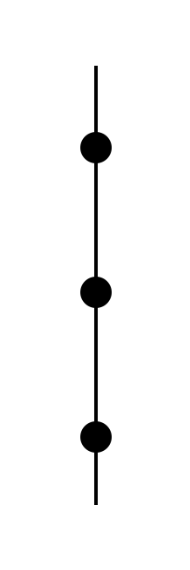
\includegraphics[width=1in]{06/06PhaseLine.png}

\item For the differential equation in problems \ref{06problem1}-\ref{06problem3} there are three equilibrium solutions. Recall that equilibrium solutions are constant functions that satisfy the differential equation. How do the other solution functions near each equilibrium solution behave in the long term? If you were to label each of these equilibrium solutions based on the way in which nearby solutions behave, what terms would you use and why? \label{06problem4} 

\end{enumerate}

\clearpage

\pagebegin{Phase Lines}

\begin{enumerate}[resume]
\item Dominique is working with the rate of change equation $\frac{dP}{dt}=0.2P$  and thinks about solutions in terms of whether they are increasing, decreasing, or remaining constant. She illustrates her thinking with the phase line shown below. 
\begin{center}
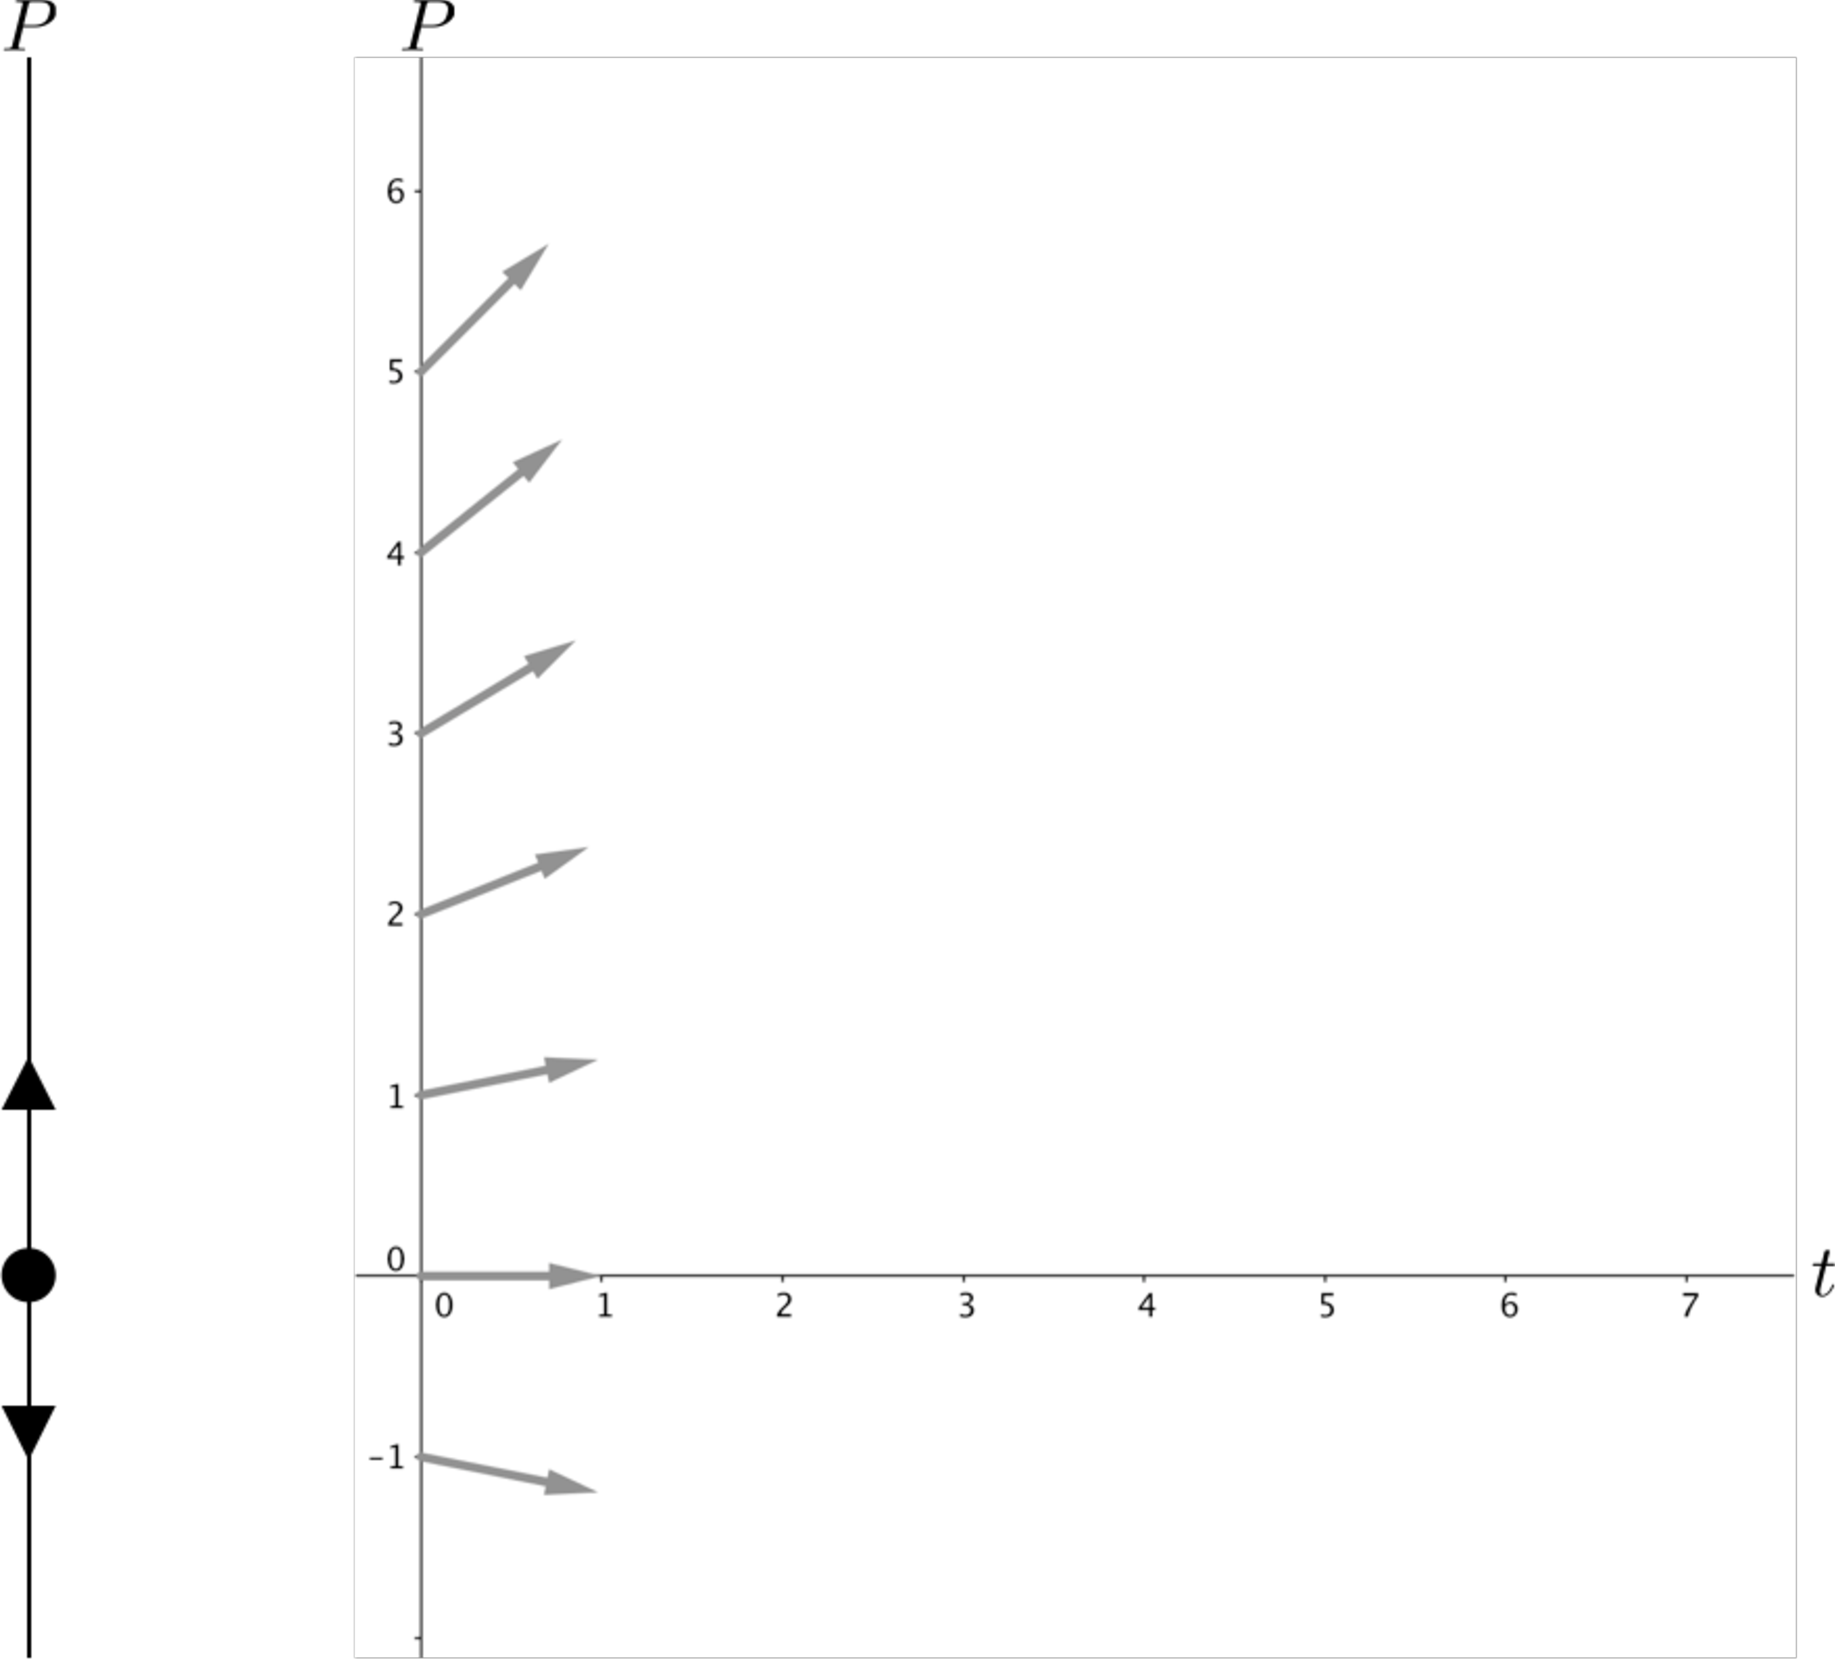
\includegraphics[width=6in]{06/06PhaseLineAndSomeVectors.pdf} \\
\end{center}
\clearpage
\begin{enumerate}
\item	Place your fingertip or other small item on the phase line at $P = 0$ and another fingertip or small item at $P = 0$ on the $P$ vs $t$ axes and imagine time moving forward. Explain, with reasons, what happens to your fingertips. \label{06problem5parta} \vfill

\item	Place your fingertip or other small item on the phase line at $P = 1$ and another fingertip or small item at $P = 1$ on the $P$ vs $t$ axes at (0,1) and imagine time moving forward. Explain, with reasons, what happens to your fingertips. \label{06problem5partb}   \vfill

\item	Place two fingertips or two small items on the phase line, one at $P = 1$ and the other at $P = 3$. What happens to your fingertips as time moves forward? How do your ideas relate to the corresponding $P$ versus $t$ graphs? \label{06problem5partc}  \vfill

\item	Explain how a person could think about the phase line as a one-dimensional projection of all of the two-dimensional $P(t)$ graphs of solutions. \label{06problem5partd} \vfill

\end{enumerate}
\end{enumerate}
\clearpage

%%%%%%%%%%%%%%%%%%%%%%%%%%%%%%%%%%%%%%%%%%%%%%%%%%%%%%%%%%%%%%%%%%%%%%%%%%%%%%%%%%%%%%%%%%
\pagebegin{Homework Set 6}

\begin{enumerate}
\item For an autonomous differential equations, it is possible to view all of the solution function graphs in terms of ``prototypical'' graphs. A prototypical solution graph represents an infinite number of other solution graphs. For example, in part (i) below one can view the entire family of functions that solve the differential equation in terms of two different prototypical solution graphs separated by an equilibrium solution: one prototypical solution graph is above the $t$-axis and one is below the $t$-axis. Each is prototypical because it can stand for all other solution graphs (in its respective region) through horizontal translation. Recall the ``Making Connections'' section of Unit 3. \label{06HWproblem1}
\begin{hnumerate}
\hitem    $\displaystyle\frac{dy}{dt}=-y$    \hitem $\displaystyle\frac{dy}{dt}=2y\left(1-\frac{y}{2}\right)$        \hitem $\displaystyle\frac{dy}{dt}=2y\left(1-\frac{y}{2}\right)+3$        \hitem   $\displaystyle\frac{dy}{dt}=y^2$ \end{hnumerate}
\begin{enumerate}
\item For each differential equation above, draw a phase line and representative graphs of solutions. \label{06HWproblem1parta}
\item For each differential equation above, explain how your response to number \ref{06HWproblem1parta} can be interpreted in terms of prototypical solutions separated by equilibrium solutions. \label{06HWproblem1partb} 
\end{enumerate}

\item For each of the following slope fields, create a differential equation whose slope field would be similar to the one given. Give reasons for why you created the differential equation as you did. You may create whatever scale on the axes that you want. \label{06HWproblem2} \\
\begin{enumerate*}
\item 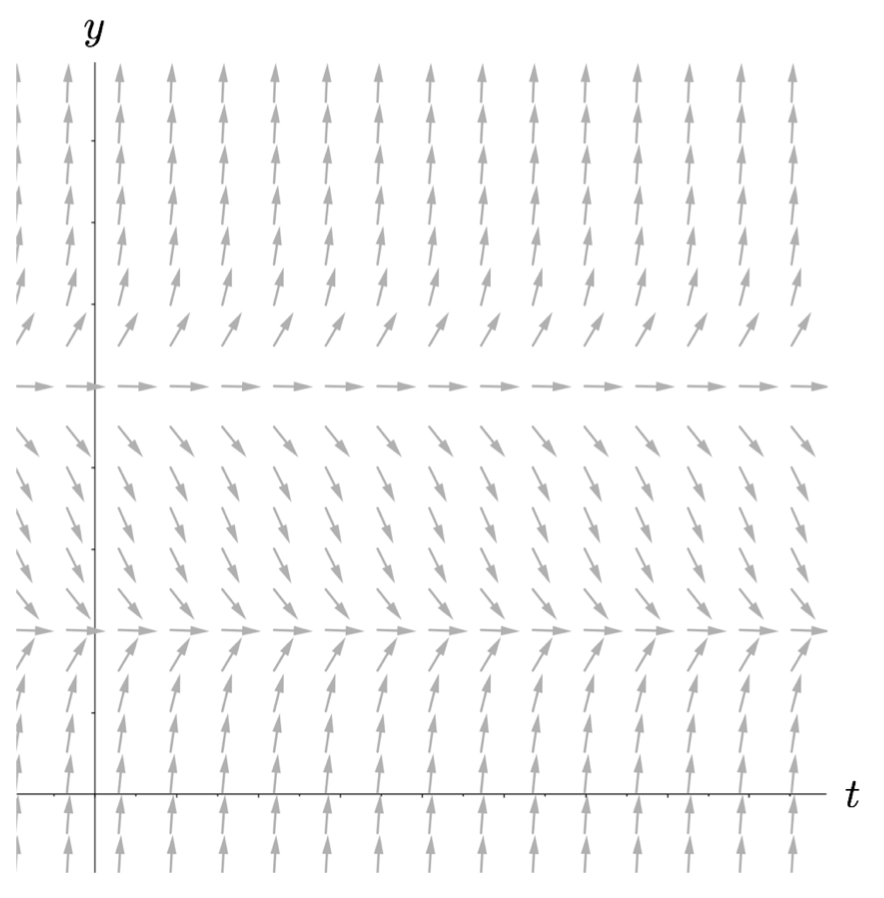
\includegraphics[width=3in]{06/06HWSlopeFieldA.png}
\item 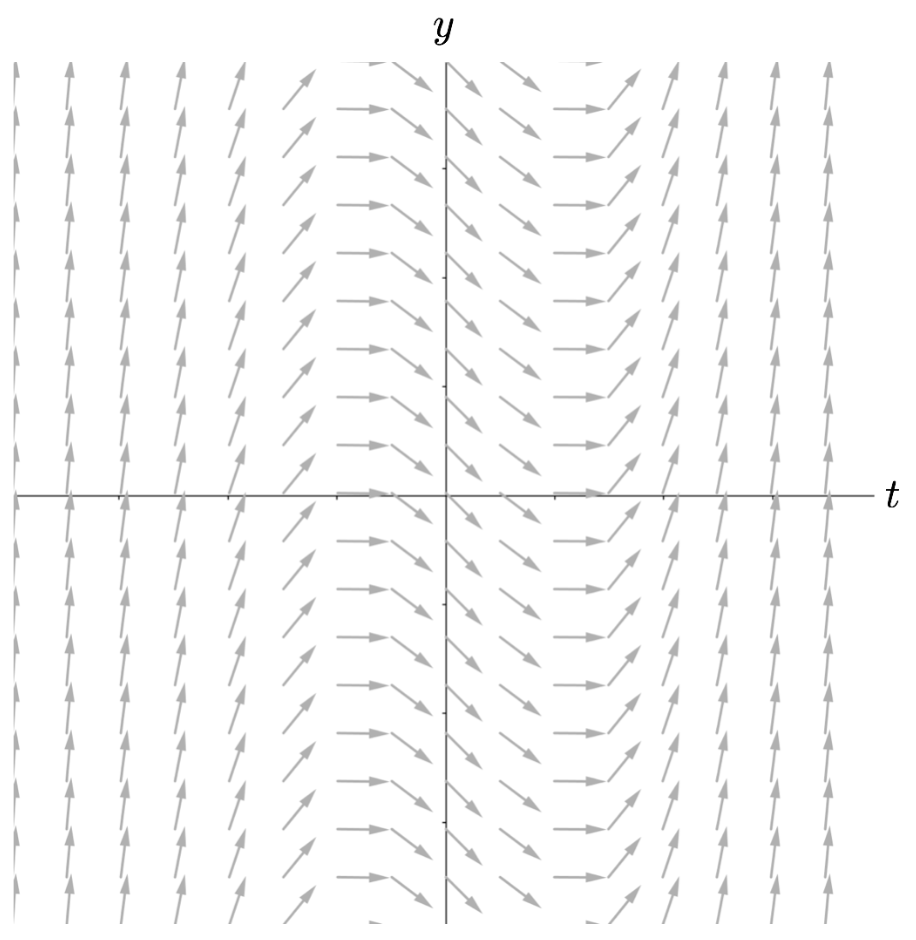
\includegraphics[width=3in]{06/06HWSlopeFieldB.png}
\item 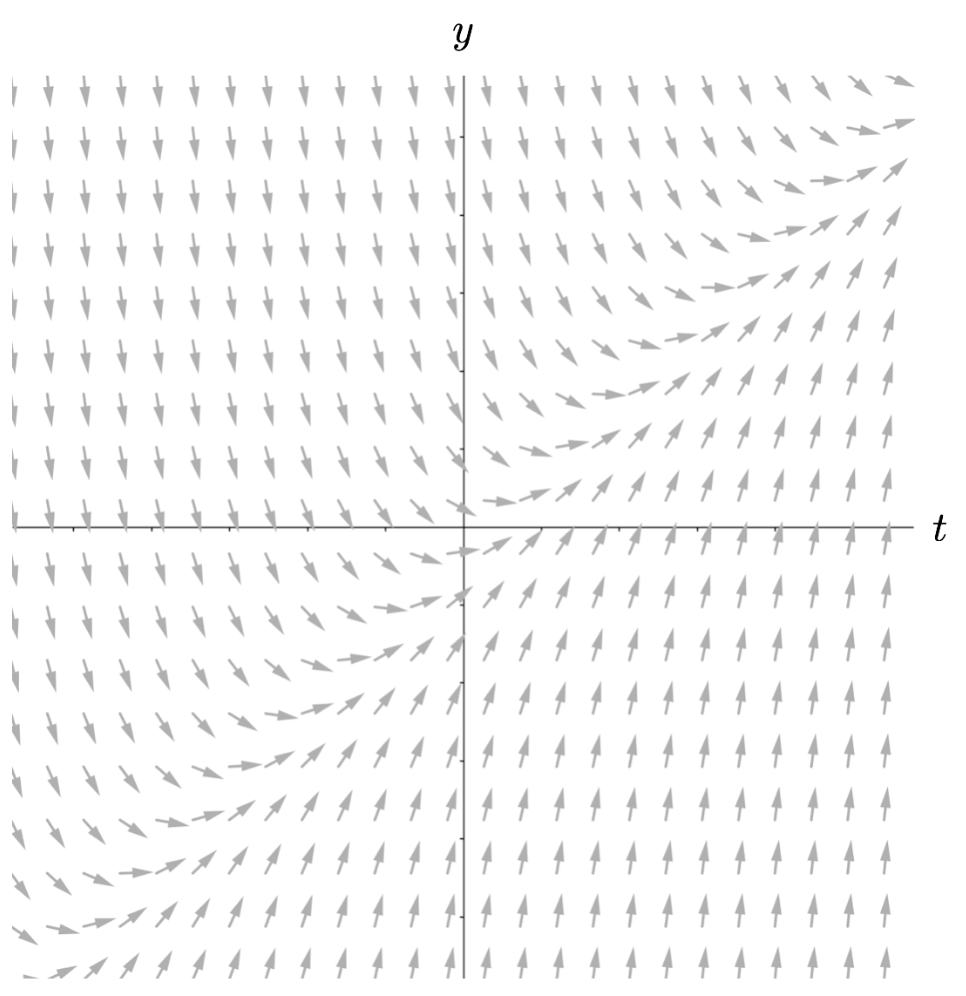
\includegraphics[width=3in]{06/06HWSlopeFieldC.png}
\item 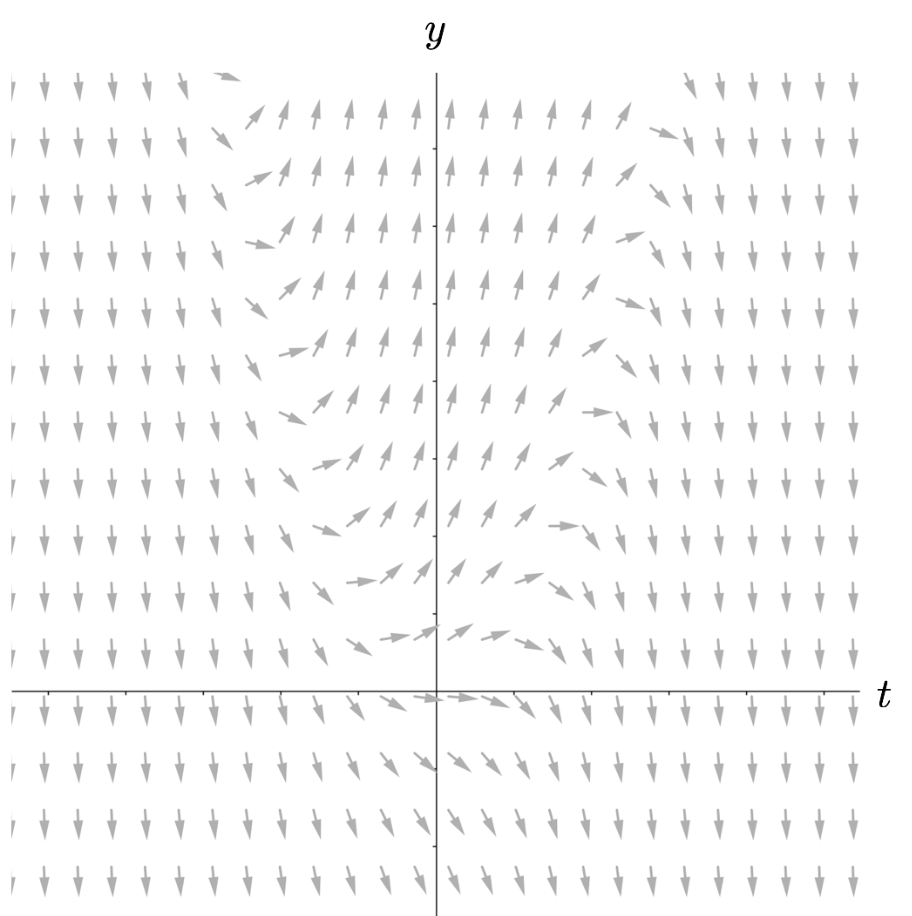
\includegraphics[width=3in]{06/06HWSlopeFieldD.png}
\end{enumerate*}

\item For each part below, create a continuous, autonomous differential equation that has the stated properties (if possible). Explain how you created each differential equation and include all graphs or diagrams you used and how you used them. If it is not possible to come up with a differential equation with the stated properties, provide a justification for why it cannot be done. \label{06HWproblem3}

\begin{enumerate}
\item Exactly three constant solution functions, two repellers and one attractor.
\item	Exactly two constant solution functions, one a repeller and one a node.
\item	Exactly two constant solution functions, both attractors.
\end{enumerate}

\item For each part below, create an autonomous differential equation that satisfies the stated criteria \label{06HWproblem4}
\begin{enumerate}
\item	$y(t)=0$ and $y(t) = -4$ are the only constant solution functions
\item $y(t)=e^{-t+1}$ is a solution
\item $y(t)=e^{2t-5}$	is a solution
\item $y(t)=10e^{0.3t}$ is a solution
\item $y(t)=1-e^{-t}$ and $y(t)=1+e^{-t}$ are solutions
\end{enumerate}

\item For a phase line to be a meaningful tool, explain why it is essential for the differential equation to be autonomous. \label{06HWproblem5}

\item In class you and your classmates continue to develop creative and effective ways of thinking about particular ideas or problems. Discuss at least one idea or way of thinking about a particular problem that has been discussed in class (either in whole class discussion or in small group) that was particularly helpful for enlarging your own thinking and/or that you disagreed with and had a different way of thinking about the idea or problem. \label{06HWproblem6}

\end{enumerate} %section 2.2 (original unit 3)
%UNIT 3: AN ANALYTIC APPROACH
%%%%%%%%%%%%%%%%%%%%%%%%%%%
%%%% Put the following at the top of each .tex file  %
\pagestyle{fancy}
\renewcommand{\theUnit}{4.1-4.2}
\ifthenelse{\isundefined{\UnitPageNumbers}}{}{\setcounter{page}{1}}
\rhead{Application  \theUnit: Population and Mixture Models}
\lhead{
\includegraphics[width=1.25cm]{IODE-logo.png}}
\rfoot{\mypage}
\lfoot{}
\cfoot{}
\fancypagestyle{firstfooter}{\footskip = 50pt}
\renewcommand{\footrulewidth}{.4pt}
%%%%%%%%%%%%%%%%%%%%%%%%%%%
\vspace*{-20pt} \thispagestyle{firstfooter}
\pagebegin{Mixture Problems (Application 4.2)}

\bbox
A one-compartment system consists of 

\bi
\ii $x(t)$ that represents the amount of a substance (such as salt) at time $t$. 
\ii an input rate of $x$. 
\ii an output rate of $x$. 
\ei

\[ \frac{dx}{dt} = \mbox{input rate} - \mbox{output rate} \]
\ebox

\bb
 \ii A brine solution of salt water that has concentration $0.05$ kg per L flows at a constant rate of 6 L per minute 
into a tank which is initially contains 50 L of a 1\% salt solution.   The brine solution flows out  of the tank at a rate of 4 L per minute. Let $x(t)$ denote the mass of the salt in the tank at time $t$ (in minutes). \textit{Note that 1\% salt solution means 1 kg of salt per 100 L of solution.}

\begin{enumerate}
\ii What is the input rate of $x$? \vspace{0.5in}
\ii What is the output rate of $x$?  \vspace{0.5in}
\ii What is the initial mass of the salt in the tank?  \vspace{0.5in}
\ii Construct an model for this initial value problem (but do not solve it).  \vspace{0.5in}
\ii What method(s) can we apply to solve the equation in (4) (but don't solve it)? 
\ee

\ee
%\bs \p 

%Now assume at time $t=0$, the tanks springs a leak so that the outflow of water is increasing linearly over time. 
%In particular, the outflow has increased from 6 L per min at time $t=0$ to 8 L per min at time $t=1$ minute. Adjust
%the differential equation to account for this leak. 

\clearpage

\pagebegin{Population Models (Section 4.1)}

\bbox
The \alert{Malthusian} law of population growth says the rate of change of the population, $\frac{dP}{dt}$,
is \alert{directly proportional to the population present}, $P$, at time $t$:
\[ \frac{dP}{dt} = kP, \quad P(0)=P_0.\]
\ebox

\bs 

\begin{ex}
 Let $P$ denote the population of the world (in billions) $t$ years since $1960$. In 1960 the world's population was approximately 3 billion, and the population growth is model by
\[ \frac{dP}{dt} =0.2P  \hspace{1in} , \ P(0)=3.\] 

Solving this model gives $P(t)=3e^{0.02t}$, and predicts the population in 2019 is $9.76$ billion.  \bs

\noindent \textbf{Why do you think predicted value is different from the actual value?}
\end{ex}

%In fact, this model predicts that in year 2635, the world's population will reach $1,800,000$ billion, meaning each person will have exactly 1 ft$^2$ of land to themself.

\clearpage

\pagebegin{The Logistic Models (Section 4.1)}

\bbox
We can construct our population model by considering::

\[ \frac{dP}{dt} = \bigg( \mbox{Birth Rate} \bigg) - \bigg( \mbox{Death Rate} \bigg).\] \bs

\bs

Competition within the population causes the populations to decrease (disease, murder, natural disasters, war, lack of food/water). If we assume the \alert{death rate is proportional to the total number of possible two-party interactions}, we get:

\[ \mbox{Death rate} = k_2 \left( \begin{array}{c} P\\ 2 \end{array} \right) = k_2 \left( \frac{P(P-1)}{2} \right) .\]

Note: $\dsty \left( \begin{array}{c} P\\ 2 \end{array} \right)$ denotes ``$P$ choose 2'', and in general we have
\[ \left( \begin{array}{c} n\\ k \end{array} \right) = \frac{n!}{k!(n-k)!}.\]
\ebox

\bs 

Taking both the birth and death rates into account, we get the \alert{Logistic model} for population change which we simplify:

\[ \frac{dP}{dt} = \bigg( \hspace{2in}  \bigg) - \bigg( \hspace{2in} \bigg) .\]  \bs

\bb[resume]
\ii Show that the model above can be rewritten in the form $\mathbf{\frac{dP}{dt} = -AP(P-L)}$ where $A$ and $L$ are positive constants.
\ee

\clearpage
\pagebegin{Practice: Population Model for Rabbits}

\bb[resume]
\ii A population of rabbits changes over time $t$ (in years) according to the logistic model
\[ \frac{dP}{dt} = 3P-\frac{1}{20}P^2 .\]

\bb
\ii For what initial population sizes $P_0$ will the population grow at first? \vspace{0.5in}
\ii For what initial population sizes $P_0$ will the population decrease at first? \vspace{0.5in}
\ii For what initial population sizes $P_0$ will the population never change? \vspace{0.5in}
\ii Explain, in practical terms, why answers in (a)-(c) makes sense. \vspace{1in}
\ii If the initial rabbit population is $P_0=P(0)=50$, find a solution to the 
initial value problem and find a formula for the population $P$ as a function of time $t$.
\ee
\ee

\pagebreak
\pagebegin{Practice: Chlorine Levels in Pool}

\bb[resume]
\ii A swimming pool whose volume is 10,000 gallons contains
water that is $0.01$\% chlorine. Starting at $t=0$, city water containing $0.001$\% chlorine
is pumped into the pool at a rate of 5 gal/min. The pool water flows out at the same rate. Let $x$
denote the amount of chlorine (in pounds) in the pool $t$ minutes since water has begun being
pumped into the pool.

\medskip

\textit{Note that a concentration of $0.01$\% chlorine solution means $0.01$ pounds of chlorine per 100 gallons of solution.}

\medskip

\bb
\ii Construct a differential equation for rate of change of the mass of chlorine (in pounds) $x$ in the pool at time $t$.  \vspace{1 in}
\ii Solve the initial value problem using the differential equation in (a) and the given initial \% concentration. \vfill
%\ii What is the percentage of chlorine in the pool after 1 hour? \vspace{1in}
\ii (Bonus) When will the pool water be $0.002$\% chlorine? 
\ee


\ee

 %Population and Salt
%UNIT 3: AN ANALYTIC APPROACH
%%%%%%%%%%%%%%%%%%%%%%%%%%%
%%%% Put the following at the top of each .tex file  %
\pagestyle{fancy}
\renewcommand{\theUnit}{4.2}
\ifthenelse{\isundefined{\UnitPageNumbers}}{}{\setcounter{page}{1}}
\rhead{Application  \theUnit: Heating and Cooling}
\lhead{
\includegraphics[width=1.25cm]{IODE-logo.png}}
\rfoot{\mypage}
\lfoot{}
\cfoot{}
\fancypagestyle{firstfooter}{\footskip = 50pt}
\renewcommand{\footrulewidth}{.4pt}
%%%%%%%%%%%%%%%%%%%%%%%%%%%
\vspace*{-20pt} \thispagestyle{firstfooter}
\pagebegin{Cooling Coffee}

%\includegraphics[]{../../IODE/Tex/Originals/07/07CoffeeCup.png}
A group of students want to develop a rate of change equation to describe the cooling rate for hot coffee in order that they can make predictions about other cups of cooling coffee. Their idea is to use a temperature probe to collect data on the temperature of the coffee as it changes over time and then to use this data to develop a rate of change equation. \\

The data they collected is shown in the table below. The temperature $C$ (in degrees Fahrenheit) was recorded every 2 minutes over a 14 minute period. \\

\begin{tabular}{|c|c|c|}
\hline
Time (min) & Temp. (\degree F) & $\frac{dC}{dt}$ (\degree F per min) \\\hline
0 & 160.3 & \ \ \ \ \ \ \ \ \ \ \ \ \ \ \ \ \ \ \ \  \\\hline
2 & 120.4 & \\\hline
4 & 98.1 &\\\hline
6 & 84.8 & \\\hline
8 & 78.5 & \\\hline
10 & 74.4 & \\\hline
12 & 72.1 & \\\hline
14 & 71.5& \\\hline
\end{tabular}
  
  \bb
  \ii Figure out a way to use this data to fill in the third column whose values approximate  $\displaystyle\frac{dC}{dt}$, where $C$ is the temperature of the coffee.\label{07problem1} 
  \item Do you expect $\displaystyle\frac{dC}{dt}$ to depend on just the temperature $C$, on just the time $t$, or both the temperature $C$ and the time $t$? \label{07problem2} 

\item Sketch below your best guess for the graph of $\displaystyle\frac{dC}{dt}$. \label{07problem3}
\begin{center}
\includegraphics[width=2.5in]{Originals/07/07dCdt.png}
\end{center}
    
\clearpage
\pagebegin{Newton's Law of Heating and Cooling}

\item \
\begin{enumerate} \label{07problem4} 
\item Input the data from your extended table in question \ref{07problem1} into the GeoGebra applet \\\href{https://ggbm.at/uj2gbz3V}{\underline{https://ggbm.at/uj2gbz3V}} to plot points for $\displaystyle\frac{dC}{dt}$ vs. $C$. Does this plot confirm or reject your sketch from question \ref{07problem3}? 
\vspace{1.5in}
\item Toggle on the curve fitting tool and find an equation that fits your data.
\end{enumerate} 
\ee

\vspace{-2in}\hspace{-0.5in}
\includegraphics[width=0.5in]{Originals/07/07CoolingCoffeeQR.png}
\vfill


\bbox
\alert{Newton's Law of Heating and Cooling} states that the temperature $T$ of an object at time $t$
changes at a rate which is proportional the difference of its temperature and the
temperature of its surrounding:
\[ \frac{dT}{dt} = -k(T-A) \]
 where $A$ is a constant that denotes the ambient temperature and $k>0$ is a constant that depends on the object.
\ebox

\bb[resume]
\ii What happens as $\mathbf{t \to \infty}$ if the initial temperature $\mathbf{T_0>A}$? If $\mathbf{T_0 < A}$? \vfill


%\ii What is/are the equilibrium solution(s)?
%\ii Find a general solution to the differential equation. Your formula for $T$ will depend on the constants $k$ and $A$ as
%well as the an arbitrary constant $C$.
%\ee

\clearpage

\pagebegin{Practice: Applications to Economics}

\ii %http://www.math.lamar.edu/faculty/maesumi/applied\%20calculus/hoffman/ch05sec03.pdf
Let $S(p)$ denote the number of units of a particular commodity supplied to the market at a price of $p$ dollars per unit, and let $D(p)$ denote the corresponding number of units demanded by the market at the same price.
\bi
\ii In static circumstances, market equilibrium occurs at the price where demand equals supply.
\ii However, certain economic models consider a more dynamic economy in which price, supply, and demand are assumed to vary with time.
\ii One of these, the Evans price adjustment model, assumes that the rate of change of price with respect to time $t$ is proportional to the shortage, which is the difference between the quantity demanded and the quantity supplied..
\ei

\bb
\ii Write a differential equation for the rate of the change of the price of the good with respect to time. \vspace{1in}
\ii If we assume that supply and demand are linear functions given by 
\[ S(p) = 2+p \ \ \ \ \mbox{ and } \ \ \ D(p)=8-2p, \]
Find a general solution to the differential equation in part (a). \vfill
\ii If the price is \$$5$ at time $t=0$ and \$$3$ at time $t=2$, determine what happens to $p$ in the long run. \vfill
\ee

\clearpage

\pagebegin{Practice: Applications to Forensic Science}

\ii %11-5y39
A detective finds a murder victim at 9 am. The temperature of the body
is measured at $90.3^{\circ}$F. One hour later, the
temperature of the body is $89.0^{\circ}$F. The
temperature of the room has been maintained at a constant
$68^{\circ}$F.
\bb
\ii Assuming the temperature, $T$, of the body obeys Newton's Law of
Cooling, write a differential equation for $T$. Your equation will include
the constant $k$ (for now). \vspace{1.25in}
\ii Solve the differential equation to estimate the time the murder occurred. \vfill
\ee
\ee
 %Heating and Cooling
%UNIT 7: MODELING WITH AUTONOMOUS DIFFERENTIAL EQUATIONS
%%%%%%%%%%%%%%%%%%%%%%%%%%%
%%%% Put the following at the top of each .tex file  %
\pagestyle{fancy}
\renewcommand{\theUnit}{7}
\ifthenelse{\isundefined{\UnitPageNumbers}}{}{\setcounter{page}{1}}
\rhead{Unit \theUnit: Modeling with Autonomous Differential Equations}
\lhead{
\includegraphics[width=1.25cm]{IODE-logo.png}}
\rfoot{\mypage}
\lfoot{}
\cfoot{}
\fancypagestyle{firstfooter}{\footskip = 50pt}
\renewcommand{\footrulewidth}{.4pt}
%%%%%%%%%%%%%%%%%%%%%%%%%%%
\vspace*{-20pt} \thispagestyle{firstfooter}
\pagebegin{Cooling Coffee}
\includegraphics[]{07/07CoffeeCup.png}
A group of students want to develop a rate of change equation to describe the cooling rate for hot coffee in order that they can make predictions about other cups of cooling coffee. Their idea is to use a temperature probe to collect data on the temperature of the coffee as it changes over time and then to use this data to develop a rate of change equation. \\

The data they collected is shown in the table below. The temperature C (in degrees Fahrenheit) was recorded every 2 minutes over a 14 minute period. \\

\begin{tabular}{|c|c|}
\hline
Time (min) & Temp. (\degree F)\\\hline
0 & 160.3\\\hline
2 & 120.4\\\hline
4 & 98.1\\\hline
6 & 84.8\\\hline
8 & 78.5\\\hline
10 & 74.4\\\hline
12 & 72.1\\\hline
14 & 71.5\\\hline
\end{tabular}
\begin{enumerate}
\item Figure out a way to use this data to create a third column whose values approximate  $\displaystyle\frac{dC}{dt}$, where $C$ is the temperature of the coffee.\label{07problem1} \vfill

\item	Do you expect $\displaystyle\frac{dC}{dt}$ to depend on just the temperature $C$, on just the time $t$, or both the temperature $C$ and the time $t$? \label{07problem2} \vfill

\item Sketch below your best guess for the graph of $\displaystyle\frac{dC}{dt}$. \label{07problem3}
\begin{center}
\includegraphics[width=3in]{07/07dCdt.png}
\end{center}

\clearpage
\item
\begin{enumerate} \label{07problem4} 
\item Input the data from your extended table in question \ref{07problem1} into the GeoGebra applet \\\href{https://ggbm.at/uj2gbz3V}{\underline{https://ggbm.at/uj2gbz3V}} to plot points for $\displaystyle\frac{dC}{dt}$ vs. $C$. Does this plot confirm or reject your sketch from question \ref{07problem3}? 
\vspace{1.5in}
\item Toggle on the curve fitting tool and find an equation that fits your data.
\end{enumerate} 

\vspace{-2in}\hspace{-0.5in}
\includegraphics[width=0.5in]{07/07CoolingCoffeeQR.png}
\vfill

\clearpage

\item One group of students figured out that a reasonable rate of change equation to be \[ \frac{dC}{dt}=-0.4C+28\]   which they rewrote as  \[\displaystyle \frac{dC}{dt}=-0.4\left(C-70\right).\] Interpret the meaning of the number $70$ in this equation. Does this rate of change equation also make sense for predicting the future temperature of a glass of ice tea? Why or why not? \label{07problem5}
\vfill
\item	According to the rate of change equation from questions \ref{07problem4} and \ref{07problem5}, is it possible for a graph of the \bf exact \rm solution to look like the one below? Why or why not? Give more than one reason for your answer. \label{07problem6}
\begin{center}
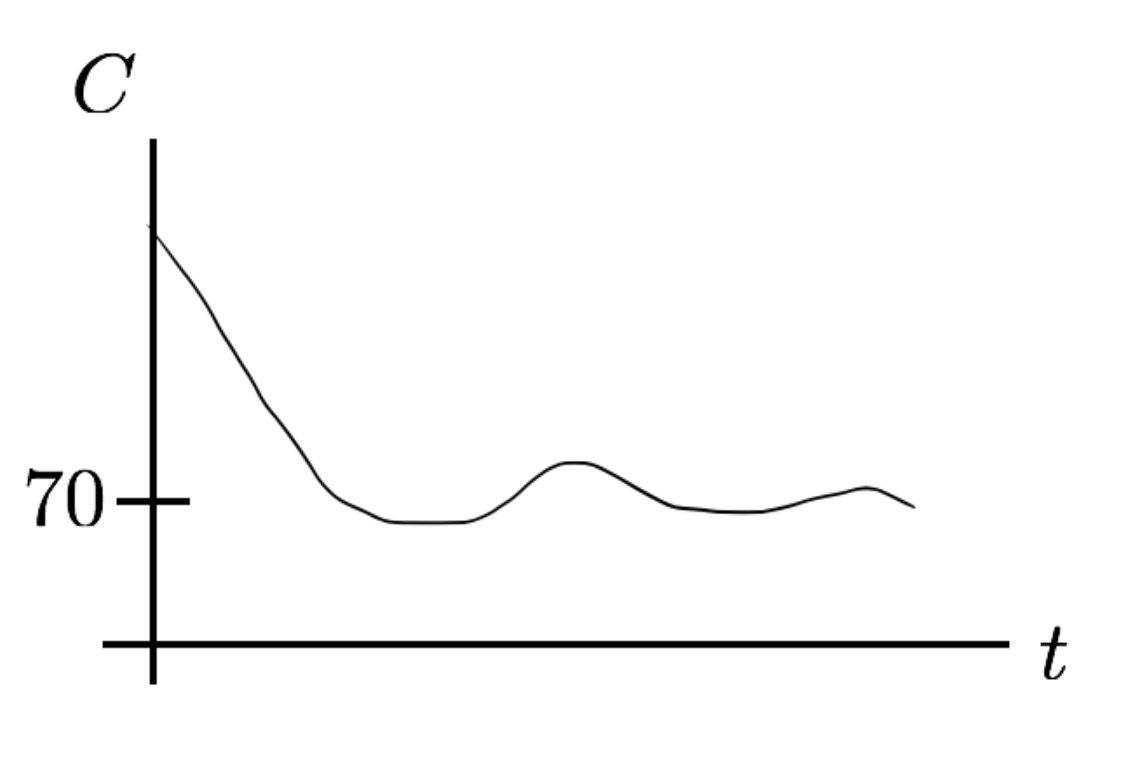
\includegraphics[width=3in]{07/07CoffeeEquilibrium.png}
\end{center}
\vfill

\end{enumerate}
\clearpage

%%%%%%%%%%%%%%%%%%%%%%%%%%%
\pagebegin{Population Growth -�� Limited Resources}

A group of biologists want to study the population growth of certain bacteria in a laboratory. The scientists realized that the culture for the bacteria does not provide unlimited resources. Hence, the rate of change equation $\displaystyle\frac{dP}{dt}=kP$ is not appropriate. They conducted experiments to determine how the rate of change of population depends on just the population. The data they collected is shown in the table below (numbers are properly scaled). At various population levels, the scientists measured the population after one day. \\

\begin{tabular}{|c|c|}
\hline
\parbox{1in}{Beginning\\ Population} & \parbox{1.5in}{Population after\\ one day}\\ \hline 
2 & 2.34\\ \hline 
4 & 4.54\\ \hline 
6 & 6.62\\ \hline 
8 & 8.58\\ \hline 
10 & 10.40\\ \hline 
12 & 12.10\\ \hline 
14 & 13.66\\ \hline 
16 & 15.10\\ \hline 
18 & 16.42\\ \hline 
20 & 17.60\\ \hline 

\end{tabular}

\begin{enumerate}[resume]
\item	Create a third column whose values approximate $\frac{dP}{dt}$. Explain why the method you used to create this column makes sense.\label{07problem7}\vfill



\item	In this course we will call a graph of $\frac{dP}{dt}$ vs. $P$, when $\frac{dP}{dt}$ is an autonomous differential equation, an \textbf{Autonomous Derivative Graph}. Create an \textbf{autonomous derivative graph} and figure out a way to analyze this graph to determine the long term behavior for each of the beginning populations given in the table above.\label{07problem8}
\vfill
\end{enumerate}

\clearpage

%%%%%%%%%%%%%%%%%%%%%%%%%%%%%%%
\pagebegin{Analyzing Graphs of Autonomous Differential Equations}

\begin{enumerate}[resume]
\item A group of biologists is studying a particular bug population in a rainforest. They gathered data about these bugs for different population values, $N$, at different times, $t$. The scientists reasoned that the rate of change depended only on the population and not on time. They approximated the derivatives $\frac{dN}{dt}$ (as was done with the cooling coffee from before) and plotted the autonomous derivative graph, as seen below: \label{07problem9}
\begin{center}
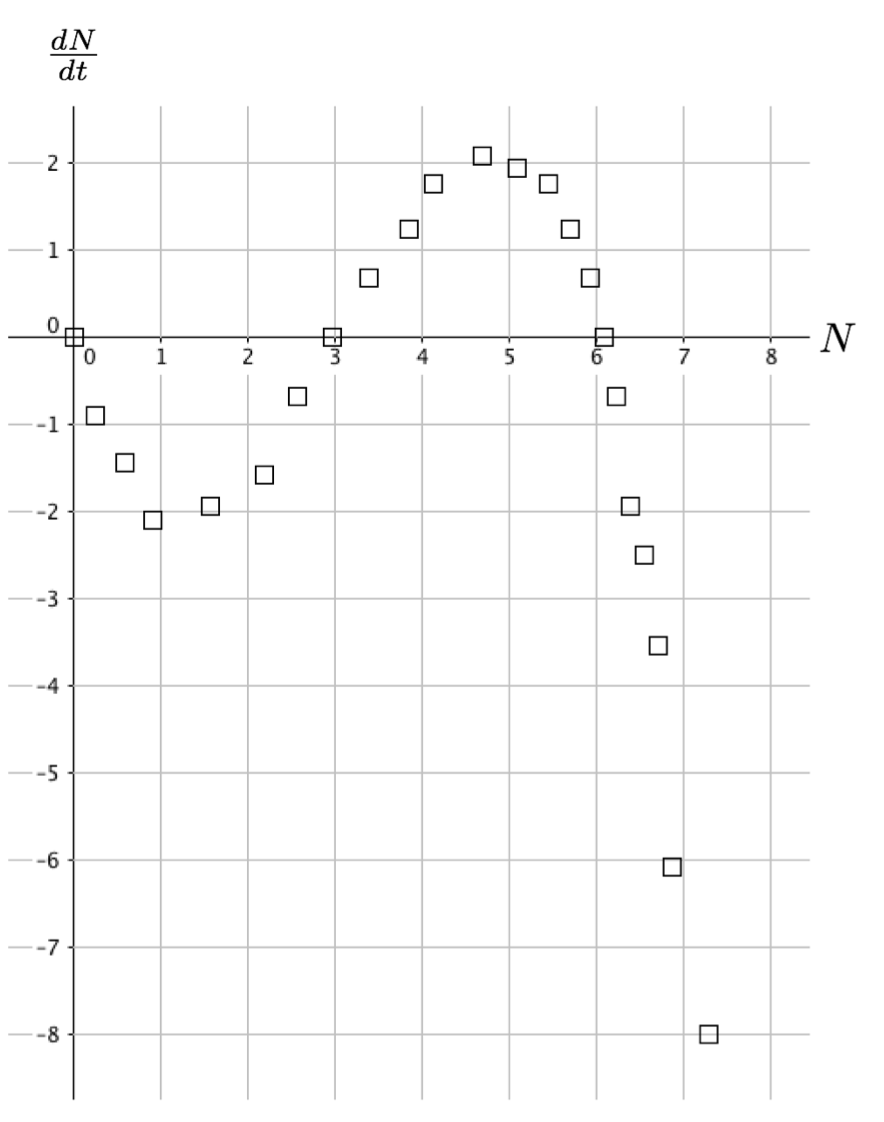
\includegraphics[width=3.5in]{07/07Bugs1.png}
\end{center}
For each part below, use the autonomous derivative graph to predict what the ultimate fate of the population will be. Describe (in words) the long-term behavior of each solution corresponding to the given initial condition. In addition, illustrate your conclusions with a suitable graph or graphs and classify all equilibrium solutions as either an attractor, repeller, or node.

\begin{enumerate}
\item	$N(0) = 2$ 
\item	$N(0) = 3$
\item	$N(0) = 4$
\item	$N(0) = 4.5$
\item	$N(0) = 6$
\item	$N(0) = 8$
\end{enumerate}

\clearpage
\item	Below is an autonomous derivative graph. Figure out the long-term behavior of \underline{every} possible solution function and illustrate your conclusions with a suitable graph or graphs. \label{07problem10}
\begin{center}
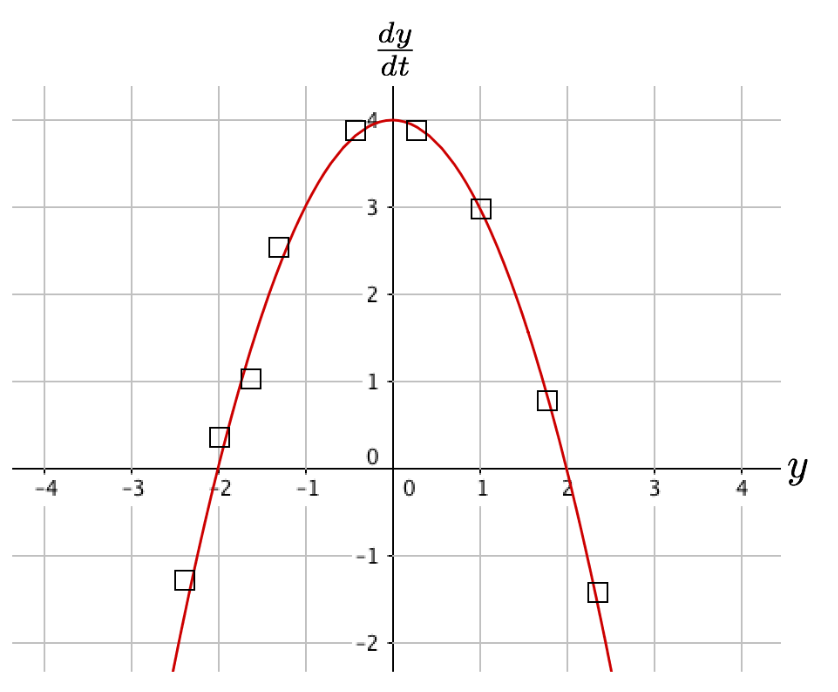
\includegraphics[width=3.5in]{07/07Bugs2.png}
\end{center}

\end{enumerate}

\clearpage
%%%%%%%%%%%%%%%%%%%%%%%%%%%%%%%%%%%%%%%%
\pagebegin{Homework Set 7}

\begin{enumerate}
\item  For this problem, use the coffee cooling rate of change equation  \[\displaystyle \frac{dC}{dt}=-0.4C+28.\] \label{07HWproblem1}
\begin{enumerate}
\item	Is there ever a time when two cups of coffee, one at initially 160\degree F and one at 180\degree F, are the exact same temperature? Answer this question according to the uniqueness theorem. Comment on whether your answer matches what you expect to happen in real life? 
\item	How long will it take a cup of hot coffee that is initially 180\degree F to cool down to 100\degree F? Use the reverse product rule to figure this out and then check the reasonableness of your answer with Euler's method.

\end{enumerate}
\item	For each part below you are provided with an autonomous derivative graph. Figure out the long-term behavior of every possible solution function. Illustrate your conclusions with representative $y(t)$ solution graphs and summarize your findings about the long-term behavior of different solutions in paragraph form. \label{07HWproblem2} \\
\begin{enumerate*}
\item 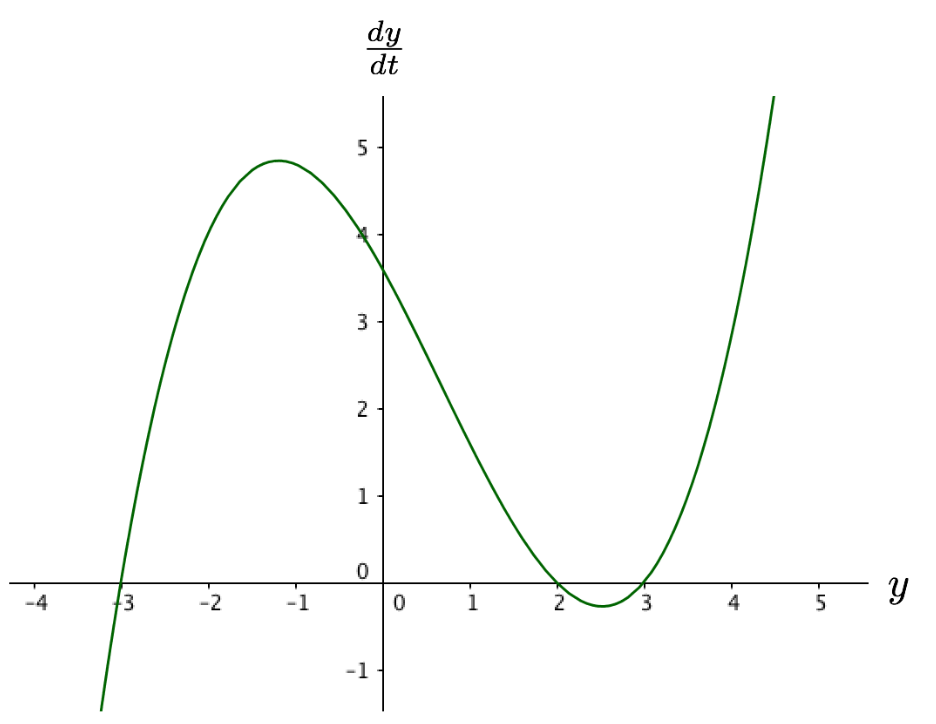
\includegraphics[width=3in]{07/07HWgraph1.png} \label{07HWproblem2parta}
\item 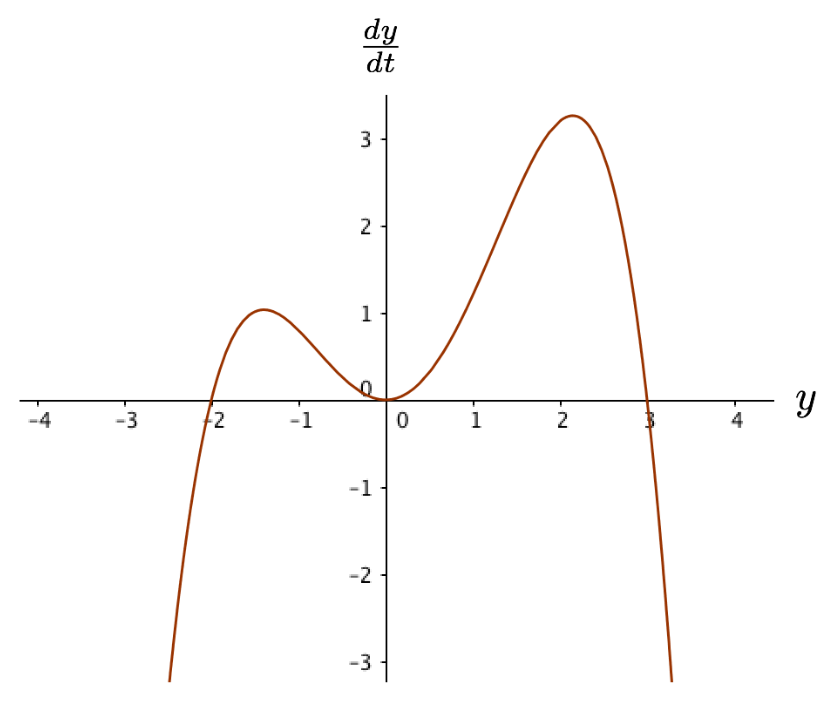
\includegraphics[width=3in]{07/07HWgraph2.png} \label{07HWproblem2partb}
\end{enumerate*}
\item	For each part in problem \ref{07HWproblem2}, create a phase line and classify each equilibrium solution as either an attractor, repeller, or node. \label{07HWproblem3}

\item	For problem \ref{07HWproblem2partb}, use the uniqueness theorem to determine if any of the non-constant solution functions ever reach the equilibrium solution of $y(t)=0$ in a finite amount of time. \label{07HWproblem4}

\item	Given an autonomous differential equation $\frac{dy}{dt}=f(y)$ , give a general strategy for how to use an autonomous derivative graph to determine the long term behavior of solution functions. \label{07HWproblem5}

\clearpage

\item	Suppose you wish to predict future values of some quantity, $y$, using an autonomous differential equation (that is, $dy/dt$ depends explicitly only on $y$). Experiments have been performed that give the following information: \label{07HWproblem6}
\begin{itemize}
\item	The only equilibrium solutions are $y(t)=0$, $y(t)=15$, and $y(t)=60$
\item	If the value of $y$ is 100, the quantity decreases
\item	If the value of $y$ is 30, the quantity increases
\item	If the value of $y$ is negative, the quantity increases
\end{itemize}

\begin{enumerate}
\item	How many different phase lines match the above? Sketch all possible phase lines. \label{07HWproblem6parta}
\item	Provide a rough sketch of an autonomous derivative graph for each of your phase lines in part \ref{07HWproblem6parta}. \label{07HWproblem6partb}
\item	For each of your different sketches in part \ref{07HWproblem6partb}, develop a differential equation that fits the basic features. \label{07HWproblem6partc}
\end{enumerate}
\item  In what ways is the letter $y$ in the differential equation $\frac{dy}{dt} = .3y$ both a variable and a function? In what ways is $\frac{dy}{dt}$ a function? \label{07HWproblem7}
\item Newton's law of cooling is an empirical law that states that an object immersed in a constant, ambient temperature will have its temperature change at a rate proportional to the difference between the its temperature and the ambient temperature. Explain how the cooling coffee problem reflects Newton's law of cooling. \label{07HWproblem8}
\item A body was found in a temperature controlled environment (i.e., you know the room temperature) and is subject to Newton's law of cooling. Explain why you only need the room temperature and the measurement of the body's temperature at two different times to give an estimate of the time of death. \label{07HWproblem9}
\end{enumerate}



 %section 4.2 (original unit 13)
%UNIT 8: THE EFFECT OF VARYING A PARAMETER IN AUTONOMOUS DIFFERENTIAL EQUATIONS
%%%%%%%%%%%%%%%%%%%%%%%%%%%
%%%% Put the following at the top of each .tex file  %
\pagestyle{fancy}
\renewcommand{\theUnit}{8}
\ifthenelse{\isundefined{\UnitPageNumbers}}{}{\setcounter{page}{1}}
\rhead{Unit \theUnit: The Effect of Varying a Parameter in Autonomous Differential Equations}
\lhead{
\includegraphics[width=1.25cm]{IODE-logo.png}}
\rfoot{\mypage}
\lfoot{}
\cfoot{}
\fancypagestyle{firstfooter}{\footskip = 50pt}
\renewcommand{\footrulewidth}{.4pt}
%%%%%%%%%%%%%%%%%%%%%%%%%%%
\vspace*{-20pt} \thispagestyle{firstfooter}
\pagebegin{Fish Harvesting}

A mathematician at a fish hatchery has been using the differential equation $\displaystyle\frac{dP}{dt}=2P\left(1-\frac{P}{25}\right)$ as a model for predicting the number of fish that a hatchery can expect to find in their pond.

\begin{enumerate}
\item Use an autonomous derivative graph, a phase line, and a slope field to analyze what this differential equation predicts for future fish populations for a range of initial conditions. Present all three of these representations and describe in a few sentences how to interpret them. \label{08problem1}
\clearpage

\item	Recently, the hatchery was bought out by fish.net and the new owners are planning to allow the public to catch fish at the hatchery (for a fee of course). This means that the previous differential equation used to predict future fish populations needs to be modified to reflect this new plan. For the sake of simplicity, assume that this new plan can be taken into consideration by including a constant, annual harvesting rate $k$ into the previous differential equation. Below are two modifications to the differential equation that may account for the new plan, as well as an option to create your own modification. Do you agree with (a) or (b)? If yes, explain why. If no, create your own modification and explain your reasoning. \label{08problem2} \\
\vs
\begin{enumerate*} 
\item $\displaystyle \frac{dP}{dt}=2P\left(1-\frac{P}{25}\right)-kP$ \hspace{.5in}
\item $\displaystyle \frac{dP}{dt}=2P\left(1-\frac{P-k}{25}\right)$ \hspace{.5in}
\item Create Your Own
\end{enumerate*}
\clearpage
	
\item	Your team of consultants settled on $\displaystyle\frac{dP}{dt} = 2P\left(1-\frac{P}{25}\right) - k$ to model the new fishing plan.  Analyze the effect of different choices for the value of k on the fish population. Synthesize your analysis in a \textbf{one page} report for the new owners that illustrates the implications that various choices of $k$ will have on future fish populations. Your report may include one or more graphical representations but must communicate the effect of different $k$ values in a concise way. \label{08problem3}

\clearpage

\item In studying climate, scientists are often concerned about positive feedback loops: two or more processes that amplify each other, creating a system of amplification that leads to a vicious cycle. One example is the interaction of water vapor with global temperature. If global temperature increases, the capacity of the atmosphere to contain evaporated water vapor also increases. If water resources are available, this would result in an increased amount of water vapor in the atmosphere. Water vapor is a greenhouse gas, thus if a climate system has more water vapor in the atmosphere, the global temperature will increase due to the increased insulation of the atmosphere. This positive feedback loop will eventually equilibrate at a higher temperature. Some scientists predict that a global increase in average temperature of just two degrees would be enough to kick off a system of positive feedback loops that would equilibrate at a temperature at least 6 degrees higher than we have now. This 6-degree increase would be enough to turn rainforests into deserts and melt ice caps. It may even redistribute the areas of the world that can support human life, i.e. making previously uninhabitable places, like the northern reaches of Siberia and Canada, inhabitable (though they may not support agriculture) and previously inhabitable places, like coastal cities, uninhabitable. \label{08problem4}

\begin{enumerate}
\item A modern pre-industrial average temperature at the equator is about 20 degrees Celsius. Assuming that our current global climate system has not undergone this vicious cycle, model this system with a phase line. What are the essential features of that phase line? \label{08problem4parta}
\vfill
\item What is a simple differential equation that corresponds to your above phase line? \label{08problem4partb}
\vfill
\clearpage
\item A group of scientists came up with the following model for this global climate system:
\[
\frac{dC}{dt} = \frac{1}{10}\Big(C-20\Big)\Big(22-C\Big)\Big(C-26\Big)-k
\]
where $C$ is the temperature, in Celsius, and $k$ is a parameter that represents governmental regulation of greenhouse gas emissions. Assume the baseline regulation corresponds to $k=0$, increasing regulation corresponds to increasing $k$, and the current equatorial temperature is around 20 degrees. To what equatorial temperature will the global climate equilibrate? \label{08problem4partc}
\vfill
\item Sketch a bifurcation diagram and use it to describe what happens to the global temperature for various values of $k$. \label{08problem4partd}
\vfill
\clearpage
\item Suppose at the start of a new governmental administration, the temperature at the equator is about 20 degrees Celsius, and $k=0$. Based on the model and other economic concerns, a government decides to deregulate emissions so that $k=-0.5$. Later, the Smokestack Association successfully lobbied for a 5\% change, resulting in $k=-0.525$. Subsequently, a new administration undid that change, reverting to $k=-0.5$, and eventually back to $k=0$. What is the equilibrium temperature at the equator after all of these changes? \label{08problem4parte}
\clearpage
\item Use your bifurcation diagram to propose a plan that will return the temperature at the equator to 20 degrees Celsius. \label{08problem4partf} \vfill

\end{enumerate}

\end{enumerate}
\clearpage
\pagebegin{Homework Set 8}

\begin{enumerate}
\item
\begin{enumerate}
\item The owners of fish.net have settled on model $dP/dt = 2 P (1-P/25) - k$ to make their business decisions, where $P$ is the number of fish in thousands, and $k$ is a harvesting rate measured in thousands of fish per year. They initially allow a harvesting rate $k = 12$. If they allow fishing to continue for a while at this rate, what does their model predict for the long term number of fish in the lake? \label{08HWproblem1parta}
\item The early years of fish harvesting went well, so they increased the harvesting rate by a modest amount.  They now allow harvesting rate corresponding to $k = 13$.  What does this model predict will be the long term result of this fishing practice? \label{08HWproblem1partb}
\item The owners of fish.net panicked when their fish population reached $P=5$ and decided to return to their original business model with $k=12$.  Will the fish population return to the levels you described in problem \ref{08HWproblem1parta}?  Why or why not? \label{08HWproblem1partc}
\end{enumerate}

\item The bifurcation diagram for an autonomous differential equation $dy/dt = f(y)$ is shown below.  The solid parts corresponds to stable equilibria and the dashed part is for unstable ones.  $f(y)$ has a parameter $c$, and changing the value of that parameter changes the behavior of the system, as shown.  \label{08HWproblem2} \\
\begin{center}
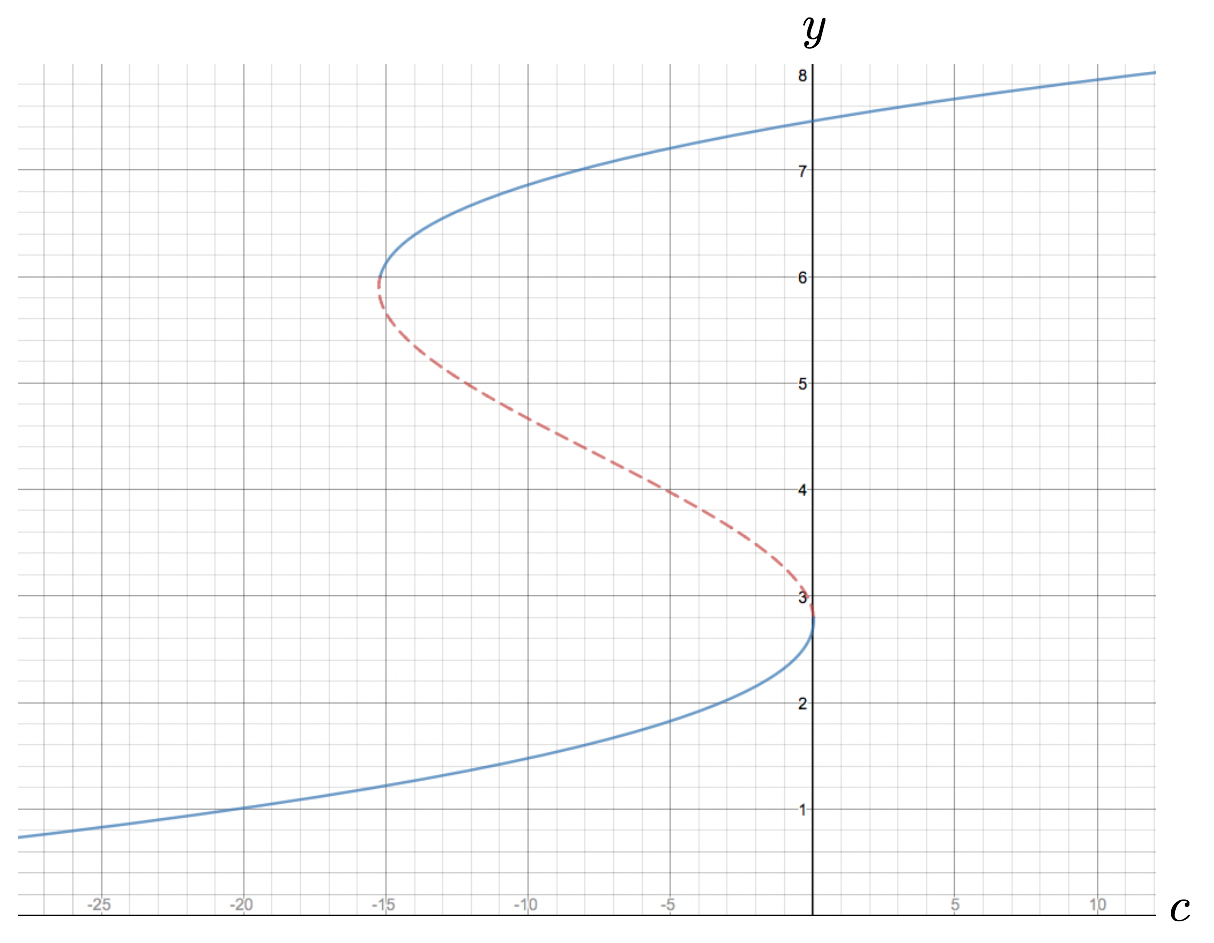
\includegraphics[width=5in]{08/08Bifurcation.png}
\end{center}
\clearpage
\begin{enumerate}
\item Sketch the phase lines when $c=-20$, $c=-5$, $c=0$, and $c=10$. \label{08HWproblem2parta}
\item Sketch the corresponding graphs of $y$ vs. $t$ for each of the choices of $c$ listed above. \label{08HWproblem2partb}
\item For what values of $c$ does the system have two attractors? \label{08HWproblem2partc}
\item As shown, the bifurcation diagram has two stable (solid) ``branches'' connected by an unstable (dashed) branch. Would it be possible for the entire curve to be stable? Why or why not?	 \label{08HWproblem2partd}
\item If this model represents a physical system, and you measure that the system has a steady state of $y = 2$, what value of $c$ should you choose for your model? \label{08HWproblem2parte}
\item Again, let's think of this model as representing some physical system, similar to the hatchery example we considered in class. You are the owner of that system, and you have control over the value of $c$. $y(t)$ represents the state of your system at a given time. Consider the following experiment. \label{08HWproblem2partf}
\begin{enumerate}
\item Let's say the system starts with an initial condition of $y(0) = 0$, and you fixed $c$ at $c = -10$. After a long time elapses, what value does $y$ approach? \label{08HWproblem2partfi}
\item Assume that $y$ has evolved to your answer in problem \ref{08HWproblem2partfi}, and that result is not something you are completely happy with. You've heard that a company down the road is using $c = 10$, so you make that change. What value does $y$ approach now (after substantial time has passed)? \label{08HWproblem2partfii}
\item Assume that $y$ has evolved now to your answer in \ref{08HWproblem2partfii}. Unfortunately, this new value of $y$ is even worse than the old one, so you want to change $c$ back to $c = -10$. Will the system evolve back to your answer in problem \ref{08HWproblem2partfi}? Explain. \label{08HWproblem2partfiii}
\end{enumerate}
\end{enumerate}

\item For each of the following, illustrate with suitable solution function graphs and/or phase lines the way in which the solutions change as the value of $r$ changes. Identify the precise value(s) of $r$ for which there is a either a change in the number of equilibrium solution(s) or a change in the type of equilibrium solution(s). Explain in words the change that happens at each significant value of $r$ identified. 

\begin{enumerate}
\item $\displaystyle \frac{dy}{dt}=(y-3)^2+r$ \label{08HWproblem3parta}
\item $\displaystyle \frac{dy}{dt}=y^2-ry+1$ \label{08HWproblem3partb}
\item $\displaystyle \frac{dy}{dt}=ry+y^3$ \label{08HWproblem3partc}
\item $\displaystyle \frac{dy}{dt}=y^6-2y^4+r$ \label{08HWproblem3partd}
\end{enumerate}

\item For problem \ref{08HWproblem3parta}, sketch a graph of the equilibrium solutions as $r$ varies. Such a graph is referred to as ``bifurcation diagram'' and the significant values of $r$ are called ``bifurcation values.'' \label{08HWproblem4}
\item For problem \ref{08HWproblem3partb}, sketch a bifurcation diagram and identify the bifurcation values. \label{08HWproblem5}
\item For problem \ref{08HWproblem3partc}, sketch a bifurcation diagram and identify the bifurcation values. Why might this bifurcation be called a ``pitchfork bifurcation?'' \label{08HWproblem6}
\end{enumerate}



 %section 4.3 (original unit 13)
%UNIT 13: SECOND ORDER LINEAR DEs
%%%%%%%%%%%%%%%%%%%%%%%%%%%
%%%% Put the following at the top of each .tex file  %
\pagestyle{fancy}
\renewcommand{\theUnit}{2.5}
\ifthenelse{\isundefined{\UnitPageNumbers}}{}{\setcounter{page}{1}}
\rhead{Section \theUnit: Nonhomogeneous Equations}
\lhead{
\includegraphics[width=1.25cm]{IODE-logo.png}}
\rfoot{\mypage}
\lfoot{}
\cfoot{}
\fancypagestyle{firstfooter}{\footskip = 50pt}
\renewcommand{\footrulewidth}{.4pt}
%%%%%%%%%%%%%%%%%%%%%%%%%%%
\vspace*{-20pt} \thispagestyle{firstfooter}
\pagebegin{Guess and Test for Nonhomogeneous Cases}

So far we have been using patterns recognized in wisely guessing the form of solutions to homogeneous second order differential equations of the form $ay''+by'+cy = 0$.  Can we adjust our guesses to handle nonhomogeneous differential equations as well?

\begin{enumerate}
\item Find a solution to the following \textbf{nonhomogeneous} differential equation:
\[
\frac{d^2x}{dt^2}+10\frac{dx}{dt}+9x=18.
\]
What is your best guess for a function whose second derivative plus 10 times its first derivative plus 9 times the function itself sum to 18? Test out your guess to see if it works. If it doesn't work keep trying. \label{13problem8}

\vfill
\end{enumerate}

The solution you found in the previous problem is called the \textbf{particular solution} to the nonhomogeneous differential equation it is not the general solution. For now we will focus on how we can find the particular solution by wisely guessing their general form based on the nonhomogeneous part of the differential equation. We will soon combine what we know about the homogeneous case and particular solutions to find general solutions. %To find the general solution to the nonhomogeneous differential equation you simply add the particular solution to the general solution to the corresponding homogeneous equation. This 3-step strategy (1 - Find the general solution to the corresponding homogeneous equation; 2 - Find the particular solution to the nonhomogeneous equation, 3 - Add the previous results) is called the \textbf{Method of Undetermined Coefficients}.

\clearpage

\begin{enumerate}[resume]
\item Find a solution to the following nonhomogeneous differential equation:
\[
\frac{d^2x}{dt^2}+10\frac{dx}{dt}+9x=18t.
\]
What is your best guess? Test out your guess to see if it works. If it doesn't work keep trying. \label{13problem8}
\vfill

\ii Based on the previous examples, what would be a good guess for the general form of the particular solution to
\[
\frac{d^2x}{dt^2}+10\frac{dx}{dt}+9x=18t^3.
\]
Your guess should have depend on constants whose values you do not need to determine for this example.
\vspace{1in}

\clearpage

\item Sean and Phil are trying to find the particular solution to $\displaystyle\frac{d^2x}{dt^2}+10\frac{dx}{dt}+9x=85\sin(2t)$. Sean guesses $x(t)=A\sin(2t)$ for the particular solution and Phil guesses $x(t)=B\cos(2t)$. \label{13problem10}

\begin{enumerate}
\item Do you think these are reasonable guesses? Explain why or why not. \label{13problem10parta} \vspace{2in}
\item For each of their guesses, can you find a value of $A$ or $B$ such that their guess is a solution? If yes, write down the general solution. If no, come up with a different guess for the particular solution and show that your guess is correct. \label{13problem10partb} \vfill
\end{enumerate}

\clearpage

\item Consider the nonhomogeneous differential equation \label{13problem15parta}
\[
\frac{d^2x}{dt^2}+25x=10\cos(5t)
\]
\bb
\ii Suppose you wish to find the particular solution to this differential equation. Explain why a guess of the form $x(t) = A\cos(5t) + B\sin(5t)$ is doomed to fail. \vspace{1in}
\item Nevertheless, explain why your particular solution must have terms that \textit{look like} $\cos(5t)$ and $\sin(5t)$. \label{13problem15partb} \vspace{1in}
\item For an unknown differentiable function $f(t)$, write down the first and second derivatives of $tf(t)$, what do you notice? \label{13problem15partc} \vspace{1in}
\item Explain why a guess of $At\cos(5t)$ is insufficient to find the particular solution. \label{13problem15partd} \vspace{1in}

\item Use the guess $x(t) = t(A\cos(5t) + B\sin(5t))$ to find a particular solution to the above equation. \label{13problem15parte} \vfill

\end{enumerate}
\end{enumerate}

\clearpage

The previous exercise is an example of \textbf{resonance}, which occurs when an external force has the same properties (such as frequency) as the general homogeneous solution. Practically speaking, when the homogeneous and nonhomogeneous parts of the differential equation have resonance this creates a huge increase in energy (that may even cause a bridge to collapse). 


\begin{enumerate}[resume]
\ii For each of the examples circle the word(s) that correctly describe whether the nonhomogeneous differential equation has resonance or not.

\bb
\ii $x''+25x=10\cos(5t)$ (\ \ \ does\ \ \  or \ \ \ does not \ \ \ ) have resonance since $x_H = C_1\cos{(5t)}+ C_2 \sin{(5t)}$.\bs
\ii $x''+25x=10e^{5t}$  (\ \ \ does\ \ \  or \ \ \ does not \ \ \ ) resonance since $x_H = C_1\cos{(5t)}+ C_2 \sin{(5t)}$. \bs
\ii $x''-3x'-10x=10\cos(5t)$  (\ \ \ does\ \ \  or \ \ \ does not \ \ \ ) resonance since $x_H = C_1e^{5t}+ C_2 e^{-2t}$. \bs
\ii $x''-3x'-10x=10e^{5t}$  (\ \ \ does\ \ \  or \ \ \ does not \ \ \ ) resonance since $x_H = C_1e^{5t}+ C_2 e^{-2t}$. \bs
\ii $x''+2x'+ 17x=6e^{-t} \sin{(4t)} $  (\ \ \ does\ \ \  or \ \ \ does not \ \ \ ) resonance since $x_H = C_1e^{-t}\cos{(4t)}+ C_2 e^{-t}\sin{(4t)}$. \bs
\ii $x''+2x'+ 17x=6 \sin{(4t)} $  (\ \ \ does\ \ \  or \ \ \ does not \ \ \ ) resonance since $x_H = C_1e^{-t}\cos{(4t)}+ C_2 e^{-t}\sin{(4t)}$. \bs
\ee

Whenever resonance is present between the homogeneous solution and nonhomogeneous forcing function, we can adjust
our initial guess by multiplying by a factor of $t$. For example, since\newline $x''+25x=10\cos(5t)$ has resonance our guess for the particular solution is
\[ x_p = t \big(  A\cos{(5t)}+ B \sin{(5t)} \big).\]

\ii For each of the examples in the previous question where there was resonance, give the initial guess for the particular solution. Do not solve for the values of the undetermined coefficients.

\vfill

\clearpage


\ii What would be a good guess for the general form of the particular solution to
\[ \frac{d^2y}{dt^2}-6\frac{dy}{dt}+9y=5e^{3t} \mbox{?}\]
Do not find the values of the undetermined coefficients. \vfill

\ii What would be a good guess for the general form of the particular solution to
\[ \frac{d^2y}{dt^2}-6\frac{dy}{dt}+9y=5e^{3t}\cos{(2t)} \mbox{?}\]
Do not find the values of the undetermined coefficients.  \vfill

\ii What would be a good guess for the general form of the particular solution to
\[ \frac{d^2y}{dt^2}-6\frac{dy}{dt}+9y=5t^2e^{3t}\cos{(2t)} \mbox{?}\]
Do not find the values of the undetermined coefficients.  \vfill



\end{enumerate}



 %section 4.4 (sort of original unit 13)
%UNIT 13: SECOND ORDER LINEAR DEs
%%%%%%%%%%%%%%%%%%%%%%%%%%%
%%%% Put the following at the top of each .tex file  %
\pagestyle{fancy}
\renewcommand{\theUnit}{2.5}
\ifthenelse{\isundefined{\UnitPageNumbers}}{}{\setcounter{page}{1}}
\rhead{Section \theUnit: General Solutions to Nonhomogeneous Second Order Linear DEs}
\lhead{
\includegraphics[width=1.25cm]{IODE-logo.png}}
\rfoot{\mypage}
\lfoot{}
\cfoot{}
\fancypagestyle{firstfooter}{\footskip = 50pt}
\renewcommand{\footrulewidth}{.4pt}
%%%%%%%%%%%%%%%%%%%%%%%%%%%
\vspace*{-20pt} \thispagestyle{firstfooter}
\pagebegin{Second Order Linear Differential Equations}

We have developed methods for finding the general homogeneous solution, $y_h(t)$, to a second order differential equation of the form
\[ ay'' + b y' + cy =0 , \ \ \ \ \mbox{for constants $a$, $b$, and $c$}:\]

\bb
\ii Write the differential equation in standard form, $ay'' + b y' + cy =0 $
\ii Set up the corresponding characteristic equation: $ar^2+br+c=0$ and find the roots.
\bi
\ii If two distinct real roots $r_1$ and $r_2$, the general solution is $y_h(t) = C_1e^{r_1t} + C_2e^{r_2t}$.
\ii If one repeated real root $r_1$, the general solution is $y_h(t) = C_1e^{r_1t} + C_2te^{r_1t}$.
\ii If complex solutions $r=\alpha \pm i \beta$, the general solution is $y_h(t) = C_1e^{\alpha t} \cos{(\beta t)} + C_2e^{\alpha t} \sin{(\beta t)}$.
\ei
\ee

We have also discussed how to find the particular solution, $y_p(t)$ to a nonhomogeneous second order differential equation of the form

\[ ay'' + b y' + cy =f(t).\] 

\bb
\ii Based on the form of $f(t)$, we guess $y_p(t)$ will have a similar form.

\begin{center}
\begin{tabular}{|c|c|}
\hline
 & \\
$f(t)$ & $y_p(t)$ \\
 & \\
\hline 
\hline
 & \\
$Ct^n$  (for $n$ a nonnegative integer) &  $A_nt^n + A_{n-1}t^{n-1}+\ldots + A_0 $  \\
 & \\
\hline
 & \\
 $Ce^{rt}$ &  $Ae^{rt}$ \\

%$\dsty Ct^m e^{rt}$ &  $\dsty \left( A_mt^m + A_{m-1}t^{m-1}+\ldots + A_0 \right)e^{rt}$ \\
 & \\
\hline
 & \\
$Ce^{\alpha t} \cos{(\beta t)}$ &  $A e^{\alpha t}\cos{(\beta t)} + B e^{\alpha t}\sin{(\beta t)}$\\
%$\dsty Ct^m e^{\alpha t}\cos{(\beta t)}$ &  $\dsty \bigg( \left( A_mt^m + A_{m-1}t^{m-1}+\ldots + A_0 \right)e^{\alpha t} \cos{(\beta t)}$\\
% & $+ \left( B_mt^m + B_{m-1}t^{m-1}+\ldots + B_0 \right)e^{\alpha t} \sin{(\beta t)} \bigg)$  \\
& \\
\hline
 & \\
 $Ce^{\alpha t} \sin{(\beta t)}$ &  $Ae^{\alpha t} \cos{(\beta t)} + B e^{\alpha t}\sin{(\beta t)}$\\
%$\dsty Ct^m e^{\alpha t}\sin{(\beta t)}$ &  Same as previous case\\
 & \\
\hline
\end{tabular}
\end{center}
\bi
\ii You have \textbf{resonance} when your initial guess for the particular solution is a homogeneous solution.
\ii When there is resonance, multiply the initial guess by $t$ (or $t^2$ if $y_h$ is a solution with a repeated real root).
\ei
\ii Plug your guess into the differential equation, and solve for the undetermined coefficients.
\ee

\clearpage
\pagebegin{Finding the General Solution to the Nonhomogeneous Case}
\bb
\ii Consider the nonhomogeneous differential equation
\[ a y''+by'+cy=f(t).\]
Let $y_h(t)$ denote the general solution to corresponding homogeneous equation $a y''+by'+cy=0$ and let $y_p(t)$ denote the particular solution for the nonhomogeneous equation. \textbf{Show that the function $y(t)=y_h(t)+y_p(t)$ is a solution to the nonhomogeneous differential equation.} \vfill

\ii Consider the differential equation
\[ \frac{d^2x}{dt^2}-\frac{dx}{dt}-12x=e^{4t}.\]
\bb
\ii Find the general homogeneous solution. \vspace{2in}
\ii Find the particular solution to the nonhomogeneous differential equation. \vfill
\ii Give the general solution to nonhomogeneous differential equation.  \vspace{1in}
\ee
\ee

\clearpage
\pagebegin{Breaking Up Sums in the Nonhomogeneous Function}

To find the general solution to the nonhomogeneous differential equation you simply add the particular solution to the general solution to the corresponding homogeneous equation. This 3-step strategy:
\bi
\ii Find the general solution to the corresponding homogeneous equation
\ii Find the particular solution to the nonhomogeneous equation
\ii Add the previous results
\ei
is called the \textbf{Method of Undetermined Coefficients}.


\begin{enumerate}[resume]
\ii Let $y_1(t)$ denote the particular solution to $ay''+by'+cy=f_1(t)$ and $y_2(t)$ denote the particular solution to $ay''+by'+cy=f_2(t)$. Show that $y_p(t) = y_1(t) + y_2(t)$ is the particular solution to $ay''+by'+cy=f_1(t)+f_2(t)$. \vfill


\ii Consider the differential equation
\[ \frac{d^2x}{dt^2}+10\frac{dx}{dt}+9x=85\sin(2t)+18.\]
Recall that we have already worked on parts of this problem. We have found that $x_h (t) = C_1e^{-9t}+C_2e^{-t}$ and the particular solution of $f_1(t) = 85\sin(2t)$ is $x_{1}(t) = -4\cos{(2t)}+\sin{(2t)}$. Using these results, finish solving the differential equation and give the general solution. \vfill

\end{enumerate}

\clearpage

\pagebegin{Products of Different Forms}

We can use the method of undetermined coefficients when the forcing function $f(t)$ is:
\bi
\ii A power function, $f(t) = Ct^n$ (for $n$ a nonnegative integer).
\ii A function of the form $f(t) = Ce^{\alpha t}\cos{(\beta t)}$ or $f(t) = Ce^{\alpha t}\sin{(\beta t)}$.
\ei

\bi
\ii For a product of a power function $t^n$ and an exponential such as $f(t) = Ct^ne^{rt}$, we guess
\[ y_p(t) = (A_n t^n + A_{n_1} t^{n-1} + \ldots A_1 t + A_0)e^{rt}\]
\bi
\ii Multiply by $t$ if $r$ is a real root  (not repeated) of the the characteristic equation.
\ii Multiply by $t^2$ if $r$ is a repeated real root of the the characteristic equation.
\ei \bs
\ei

\bb[resume]
\ii Give a guess for the particular solution to
\[ y'' - 5y' -6y = 4t^2e^{6t}.\] \vfill
\ee


%\ii For a product of an exponential and either a sine or cosine such as $f(t) = Ce^{\alpha t}\cos{(\beta t)}$ or \newline $f(t) = Ce^{\alpha t}\sin{(\beta t)}$, we guess
%\[ y_p(t) =Ae^{\alpha t}\cos{(\beta t)} + Be^{\alpha t}\sin{(\beta t)} \]
%\bi
%\ii Multiply by $t$ if $\alpha \pm i \beta$  are the complex roots of the the characteristic equation.
%\ei \vfill
%\ii For a product of a power function $t^n$ and either a sine or cosine such as $f(t) = Ct^n\cos{(\beta t)}$ or \newline $f(t) = Ct^n\sin{(\beta t)}$, we guess
%\[ y_p(t) =(A_n t^n + A_{n_1} t^{n-1} + \ldots A_1 t + A_0)\cos{(\beta t)} + (B_n t^n + B_{n_1} t^{n-1} + \ldots B_1 t + B_0)\sin{(\beta t)} \]
%\bi
%\ii Multiply by $t$ if $0 \pm i\beta$  are the complex roots of the the characteristic equation.
%\ei \vfill
\bi
\ii For a product of a power function, an exponential, and either a sine or cosine such as \newline $f(t) = Ct^ne^{\alpha t}\cos{(\beta t)}$ or $f(t) = Ct^ne^{\alpha t}\sin{(\beta t)}$, we guess
\[ y_p(t) =(A_n t^n + A_{n_1} t^{n-1} + \ldots A_1 t + A_0)e^{\alpha t}\cos{(\beta t)} + (B_n t^n + B_{n_1} t^{n-1} + \ldots B_1 t + B_0)e^{\alpha t}\sin{(\beta t)} \]
\bi
\ii Multiply by $t$ if $\alpha \pm i \beta$  are the complex roots of the the characteristic equation.
\ei \bs
\ei

\bb[resume]
\ii Give a guess for the particular solution to
\[ y'' - 5y' -6y = 4t^2e^{6t}\sin{t}.\] \vfill
\ee


\clearpage

\begin{enumerate}[resume]

\ii Consider the differential equation $x''-8x'+12x=f(t)$. For each $f(t)$, what would be your guess for the particular solution? Do not solve for the undetermined coefficients. If the method of undetermined coefficients cannot be applied, explain why not.

\bb
\ii $f(t) = 10\sin{(2t)}$ \vfill

\ii $f(t) = 10e^{6t}\sin{(2t)}$ \vfill

\ii $f(t) = 10\tan{(2t)}$ \vfill

\ii $f(t) = 10te^{2t}$ \vfill

\ii $f(t) = 8t^{-2}$ \vfill

\ii $f(t) = 6te^{5t}\cos{(3t)}$ \vfill

\ee

\ee
 %section 4.5 (sort of original unit 13)
%UNIT 3: AN ANALYTIC APPROACH
%%%%%%%%%%%%%%%%%%%%%%%%%%%
%%%% Put the following at the top of each .tex file  %
\pagestyle{fancy}
\renewcommand{\theUnit}{2.4}
\ifthenelse{\isundefined{\UnitPageNumbers}}{}{\setcounter{page}{1}}
\rhead{Section \theUnit: Mechanical Vibrations}
\lhead{
\includegraphics[width=1.25cm]{IODE-logo.png}}
\rfoot{\mypage}
\lfoot{}
\cfoot{}
\fancypagestyle{firstfooter}{\footskip = 50pt}
\renewcommand{\footrulewidth}{.4pt}
%%%%%%%%%%%%%%%%%%%%%%%%%%%
\vspace*{-20pt} \thispagestyle{firstfooter}

\pagebegin{Free Damped Motion}
\bb
\ii Consider a mass-spring system with a mass $m=2$, spring constant $k=3$, and damping constant $b=1$.
\bb
\ii Set up and find a general solution to the corresponding differential equation.
\ii Is the system underdamped, overdamped, or critically damped?
\ii Find a value for the constant $b$ so sytem is critically damped.
\ii What is the period of solution? How many cycles does the mass-spring complete each second?
\ee

\vfill

\bbox
For these problems we will measure quantities using the metric system:
\bi
\ii The overall force is measured in newtons, $N$.
\bi
\ii It is equal to the force that would give a mass of one kilogram an acceleration of one meter per $\mbox{sec}^2$,
\ei
\ii The spring constant $k$ has units of force per unit of distance. For example newtons per meter, N/m.
\ii The damping constant is a unit of impulse per unit of distance. For example newton seconds per meter, $\mbox{N} \cdot \mbox{s}$ per meter.
\ei
\ebox

\newpage

\ii You place an object whose mass $m$ (in kg) is unknown on top of a spring and put the system in motion. You observed the mass bounce up and down. Let $y$ denote the vertical distance of the mass from its equilibrium position, with $y>0$ when the mass is stretched above the equilibrium.

\bb
\ii If we ignore friction, then the location of the mass $y$ follows the same model for the undamped free mass-spring system:
\[ my''+ky=0.\]
If the spring constant of the spring is $k=4 \mbox{ N/m}$, then give a solution to the initial value problem. Note your answer will depend on the mass $m$.
\ii  If the mass bounces with a frequency of $0.8$ cycles per second, then give the value of the mass $m$.
Note that one cycle means the mass goes from equilibrium, down, then back up, and returns to equilibrium. 
\ee


\newpage

\ii A 5000 kg railcar hits a spring bumper at a speed of 1 meter per second, and the spring compresses by $0.1$ m. Assume no damping.
\bb
\ii Find the value of the spring constant $k$.
\ii How far does the spring compress when a $10,\!000$ kg railcar hits the spring at the same speed?
\ii If the spring would break if it compresses more than $0.3$ m, what is the maximum mass of a railcar that can hit at 1 m/s?
\ii What is the maximum mass of a railcar that can hit the spring without breaking it at a speed of 2 m/s.
\ee


\newpage

\pagebegin{Section 2.6: Forced Oscillations}


\ii A water tower in an earthquake acts as a mass-spring system. Assume the the container on top is full and the water does not move around. The container is the mass, and the support is the spring. The container with the water has a mass of $10,\!000$ kg. It takes a force of 1000 newtons to displace the container 1 meter. For simplicity, we assume no friction. The earthquake induces an external force given by $F(t)=m\omega^2\cos{(\omega t)}$ where $\omega$ denotes the frequency (number of cycles per second). When the earthquake hits, the water tower is at rest.

\bb
\ii What is the natural frequency of the water tower? This means, if there is no external force (homoegenous), what is the frequency of the homogeneous solution?
\ii If the water tower moves more than $1.5$ meters from its equilbrium resting position, the tower will collapse. Suppose an earthquake with a frequency of $0.5$ cycles per second hits, will the water tower collpase or remain standing?
\ee

\ee
 %Applications of 2nd order
%UNIT 11: DAMPED AND UNDAMPED LINEAR SYSTEMS
%%%%%%%%%%%%%%%%%%%%%%%%%%%
%%%% Put the following at the top of each .tex file  %
\pagestyle{fancy}
\renewcommand{\theUnit}{11}
\ifthenelse{\isundefined{\UnitPageNumbers}}{}{\setcounter{page}{1}}
\rhead{Unit \theUnit: Damped and Undamped Linear Systems}
\lhead{\includegraphics[width=1.25cm]{IODE-logo.png}}
\rfoot{\mypage}
\lfoot{}
\cfoot{}
\fancypagestyle{firstfooter}{\footskip = 50pt}
\renewcommand{\footrulewidth}{.4pt}
%%%%%%%%%%%%%%%%%%%%%%%%%%%
\vspace*{-20pt} \thispagestyle{firstfooter}
\pagebegin{Spiraling Solutions - Spring Mass Revisited}

In a previous problem we applied Newton's law of motion for a spring mass system and obtained the second order differential equation  $\displaystyle \frac{d^2x}{dt^2}+\frac{b}{m}\frac{dx}{dt}+\frac{k}{m}x=0$, where $x$ is the position of the object attached to the end of the spring, $m$ is the mass of the object, $b$ is the damping coefficient, and $k$ is the spring constant. Using the fact that velocity is the derivative of position and choosing the mass $m = 1$ and the spring constant $k = 2$, we converted this to the following system of two differential equations:  
\begin{center}
\raisebox{1.5\height}{$\displaystyle \begin{aligned}
\frac{dx}{dt}&=y \\ \frac{dy}{dt}&= -2x-by
\end{aligned}$} \hspace{1in}\includegraphics[width=2in]{11/11SpringMass.png}
\end{center}

We were able to figure out the $x(t)$ and $y(t)$ equations when the value of the friction parameter was such that there were straight line solutions in the phase plane. Such a situation is typically referred to as \textit{overdamped}. The situation is called \textit{damped} when the differential equations predict that the mass will oscillate about the 0 position and \textit{undamped} when there is no friction. In the following problems we figure out the $x(t)$ and $y(t)$ equations for the damped. We consider the undamped situation in the homework. \\

The vector field for the case when $b = 2$ is shown below. Based on this vector field, it appears that the differential equations predict that the mass will oscillate back and forth. Even though there are not any straight line solutions, we can still use the same algebraic approach as before to get the $x(t)$ and $y(t)$ equations for any initial condition, but we will have to deal complex numbers. Problems \ref{11problem1}-\ref{11problem7} outline a way to do this.
\begin{center}
\includegraphics[width=3.5in]{11/11figure.png}
\end{center} 

\clearpage
\begin{enumerate}
\item	For the system of differential equations 
\begin{align*}
\frac{dx}{dt}&=y \\ \frac{dy}{dt}&= -2x-2y
\end{align*}
use the same algebraic approach as before to verify that the slopes of the ``straight line'' solutions are $-��1 \pm i$. \label{11problem1} \vfill

\item	For solutions with ``straight line'' slope $y=(-1+i)x$, find the $x(t)$ and $y(t)$ equations (in terms of complex numbers) for the solution along this ``straight line''�� with initial condition $(1, -1+i)$.\label{11problem2} \vfill

\clearpage

\item	For solutions with ``straight line'' slope  $y=(-1-i)x$, find the $x(t)$ and $y(t)$ equations (in terms of complex numbers) for the solution along this ``straight line'' with initial condition $(1, -1-i)$.\label{11problem3} \vfill

\item	Use Euler's formula $e^{a+ib}=e^ae^{ib}=e^a(\cos b+i\sin b)$ to rewrite the $x(t)$ and $y(t)$ equations from problem \ref{11problem2} (call these $x_1(t)$ and $y_1(t)$) and then again from problem \ref{11problem3} (call these $x_2(t)$ and $y_2(t)$). \label{11problem4} \vfill

\clearpage

\item	Denise suggests that if you add $\displaystyle \begin{pmatrix}
x_1(t)\\y_1(t)
\end{pmatrix}$ to $\displaystyle \begin{pmatrix}
x_2(t)\\y_2(t)
\end{pmatrix}$  the resulting pair of equations is (i) real valued and (ii) a solution to the same system of differential equations. Verify that this is true. \label{11problem5} \vfill

\item	Verify that if you subtract $\displaystyle \begin{pmatrix}
x_1(t)\\y_1(t)
\end{pmatrix}$  from $\displaystyle \begin{pmatrix}
x_2(t)\\y_2(t)
\end{pmatrix}$ and multiply the result by the complex number $i$, then the resulting pair of equations will be a real and a solution to the same system of differential equations. \label{11problem6} \vfill

\clearpage

\item	\label{11problem7}
\begin{enumerate}
\item Form the general solution to the system of differential equations 
\begin{align*}
\frac{dx}{dt}&=y \\ \frac{dy}{dt}&= -2x-2y
\end{align*}
\item What aspect of your general solution could be interpreted as the effect of friction on the spring mass system?
\item Find the particular solution for the initial condition (2, 3) and sketch the $x$ vs $t$ and $y$ vs $t$ graphs. 
\end{enumerate}
\end{enumerate}

\clearpage

%%%%%%%%%%%%%%%%%%%%%%%%%%%%%%%%%%%%%%%%%%%%%%
\pagebegin{Homework Set 11}

\begin{enumerate}
\item	The general solution to \label{11HWproblem1}
\begin{align*}
\frac{dx}{dt}&=y\\
\frac{dy}{dt}&= -2x-2y
\end{align*}
is
\begin{align*}
x(t) &= c_1e^{-t}\cos(t)+c_2e^{-t}\sin(t) \\
y(t) &= c_1e^{-t}(-\cos(t)-\sin(t))+c_2e^{-t}(-\sin(t)+\cos(t))
\end{align*}
Which part(s) of the general solution accounts for the fact that the differential equations predict that the mass will oscillate about the zero position? Which part(s) of the general solution accounts for the fact that the amplitude of the oscillations decreases over time?

\item	Suppose that for a different system of differential equations you got the exact same general solution as homework problem 1 except instead of $e^{-t}$ you got $e^t$. How would this change graphs of solutions in the phase plane? Explain. \label{11HWproblem2} 

\item	Find the general solution to the spring mass problem when there is no friction. Sketch these solution in the phase plane and explain how this general solution fits with your expectation for the behavior of the mass over time. Note: when there is no friction, $b = 0$, and the spring constant $k = 2$, we get \label{11HWproblem3}    
\begin{align*}
\frac{dx}{dt}&=y\\ \frac{dy}{dt}&= -2x
\end{align*}

\clearpage

\item Consider the phase planes below: \label{11HWproblem4} \\
\begin{enumerate*}
\item[(A)] \includegraphics[width=2.5in]{11/11HWVectorField1.png}
\item[(B)] \includegraphics[width=2.5in]{11/11HWVectorField2.png} \\
\item[(C)] \includegraphics[width=2.5in]{11/11HWVectorField3.png}
\item[(D)] \includegraphics[width=2.5in]{11/11HWVectorField4.png}
\end{enumerate*}

For each sentence below, fill in the blank with choices from the following two lists:

\begin{center}
\begin{tabular}{ccccc}
\textbf{\underline{Spring System (First Blank)}} &&& \textbf{\underline{Solutions (Second Blank)}} \\
a damped spring &&& $c_1\cos(t) + c_2\sin(t)$ \\
an overdamped spring &&& $e^{-t}(c_1\cos(t) + c_2\sin(t))$ \\
an undamped spring &&& $e^{t}(c_1\cos(t) + c_2(\sin(t))$ \\
something other than a spring &&& $c_1 e^t + c_2 e^{2t}$ \\
&&& $c_1 e^{-t} + c_2 e^{-2t}$ \\
&&& $c_1 e^{-t} + c_2 e^{2t}$ \\
&&& $c_1 e^t + c_2 e^{-2t}$	
\end{tabular}
\end{center}

Phase plane (A) corresponds to \rule{1in}{.5pt} and the solutions look like $x(t)$=\rule{1.5in}{.5pt} \\

Phase plane (B) corresponds to \rule{1in}{.5pt} and the solutions look like $x(t)$=\rule{1.5in}{.5pt} \\

Phase plane (C) corresponds to \rule{1in}{.5pt} and the solutions look like $x(t)$=\rule{1.5in}{.5pt} \\

Phase plane (D) corresponds to \rule{1in}{.5pt} and the solutions look like $x(t)$=\rule{1.5in}{.5pt}

\clearpage

\item What type of system (undamped, damped, overdamped) do the following best correspond to? Explain your reasoning. \label{11HWproblem5}
\begin{enumerate}
\item A car that bounces every time it hits a bump
\item A pendulum immersed in a vat of honey
\item A bungee jumper
\end{enumerate}

\item In each part, write a differential equation corresponding to the given scenario: \label{11HWproblem6}
\begin{enumerate}
\item An undamped spring
\item An underdamped spring
\item An overdamped spring
\end{enumerate}

\item Does Adding Solutions Always Result in Another Solution? \\

In deriving the general solution to the spring mass problem, two solutions were added to get another solution. This worked for the particular equations at hand, but does adding two solutions to a system of differential equations of the form    
\begin{align*}
\frac{dx}{dt}&=ax+by\\ \frac{dy}{dt}&= cx+dy
\end{align*}
 always result in another solution to the same system of differential equations? Below is a proof that this in fact is true.

\noindent \underline{Claim}:
If  $\displaystyle \begin{pmatrix}
x_1(t)\\y_1(t)
\end{pmatrix}$  and $\displaystyle \begin{pmatrix}
x_2(t)\\y_2(t)
\end{pmatrix}$  are solutions (not necessarily straight line solutions) to a system of differential equations of the form  \begin{align*}\begin{split}
\frac{dx}{dt}&=ax+by\\ \frac{dy}{dt}&= cx+dy
\end{split}\end{align*}
 then the sum of these two solutions is also a solution. That is, if we call the sum of these two solutions  $\displaystyle \begin{pmatrix} x_3(t)\\y_3(t) \end{pmatrix}$ where 
 \[ \begin{pmatrix}
x_3(t)\\y_3(t)
\end{pmatrix}=\begin{pmatrix}
x_1(t)\\y_1(t)
\end{pmatrix}+\begin{pmatrix}
x_2(t)\\y_2(t)
\end{pmatrix}=\begin{pmatrix}
x_1(t)+x_2(t)\\y_1(t)+y_2(t)
\end{pmatrix},\]
 then  $\displaystyle \begin{pmatrix} x_3(t)\\y_3(t) \end{pmatrix}$  is also a solution to the same system of differential equations.  

\noindent\underline{Proof:}
In order to show that $\displaystyle \begin{pmatrix} x_3(t)\\y_3(t) \end{pmatrix}$  is a solution, we need to verify it satisfies the system of differential equations. This is, we need to show that  
\begin{align*}\begin{split}
\frac{d}{dt}x_3(t)&=ax_3(t)+by_3(t)\\ \frac{d}{dt}y_3(t)&= cx_3(t)+dy_3(t)
\end{split}.\end{align*}

Since   
\[ \begin{pmatrix}
x_3(t)\\y_3(t)\end{pmatrix}=\begin{pmatrix}
x_1(t)+x_2(t)\\y_1(t)+y_2(t)
\end{pmatrix},\] we know that   
\begin{align}\begin{split}
\frac{d}{dt}x_3(t)&=\frac{d}{dt}x_1(t)+\frac{d}{dt}x_2(t)\\ \frac{d}{dt}y_3(t)&= \frac{d}{dt}y_1(t)+\frac{d}{dt}y_2(t) 
\end{split}.\label{12HWeqn1}\end{align}
Because $\displaystyle \begin{pmatrix} x_1(t)\\y_1(t) \end{pmatrix}$   is a solution, it satisfies the system of differential equations. That is,    
\begin{align}\begin{split}
\frac{d}{dt}x_1(t)&=ax_1(t)+by_1(t)\\ \frac{d}{dt}y_1(t)&= cx_1(t)+dy_1(t) \label{12HWeqn2}
\end{split}\end{align}  
Similarly, since   $\displaystyle \begin{pmatrix} x_2(t)\\y_2(t) \end{pmatrix}$   is a solution,  
  
\begin{align}\begin{split}
\frac{d}{dt}x_2(t)&=ax_2(t)+by_2(t)\\ \frac{d}{dt}y_2(t)&= cx_2(t)+dy_2(t) \label{12HWeqn3}
\end{split}\end{align}  

Substituting \eqref{12HWeqn2} and \eqref{12HWeqn3} into \eqref{12HWeqn1} yields 
\begin{align*}\begin{split}
\frac{d}{dt}x_3(t)&=ax_1(t)+by_1(t)+ax_2(t)+by_2(t)\\ \frac{d}{dt}y_3(t)&= cx_1(t)+dy_1(t)+cx_2(t)+dy_2(t) 
\end{split}.\end{align*}  
Rearranging terms yields
\begin{align*}\begin{split}
\frac{d}{dt}x_3(t)=ax_1(t)+ax_2(t)+by_1(t)+by_2(t) &= a[x_1(t)+x_2(t)]+b[y_1(t)+y_2(t)] \\ \frac{d}{dt}y_3(t)= cx_1(t)+cx_2(t)+dy_1(t)+dy_2(t) &= c[x_1(t)+x_2(t)]+d[y_1(t)+y_2(t)] 
\end{split}.\end{align*}  


Finally, using the fact that   \[ \begin{pmatrix}
x_3(t)\\y_3(t)\end{pmatrix}=\begin{pmatrix}
x_1(t)+x_2(t)\\y_1(t)+y_2(t)
\end{pmatrix},\]   yields \begin{align*}\begin{split}
\frac{d}{dt}x_3(t)&=ax_3(t)+by_3(t)\\ \frac{d}{dt}y_3(t)&= cx_3(t)+dy_3(t)
\end{split}\end{align*}
   which is what we set out to show. Therefore $\displaystyle  \begin{pmatrix}
x_3(t)\\y_3(t)\end{pmatrix}$  is also a solution to the system of differential equations.

\clearpage

\begin{enumerate}
\item	Suppose that \label{12HWprob7parta} $\displaystyle  \begin{pmatrix}
x_1(t)\\y_1(t)\end{pmatrix}$  and $\displaystyle  \begin{pmatrix}
x_2(t)\\y_2(t)\end{pmatrix}$  are solutions to the system of differential equations
\begin{align*}\begin{split}
\frac{dx}{dt}&=ax+by+1\\ \frac{dy}{dt}&= cx+dy+2
\end{split}\end{align*}
 where $a, b, c,$ and $d$ are constants. Josh claims that the sum of these two solutions is also a solution to the same system of differential equations. Do you agree with his claim? Either develop a similar proof as above to support this claim or point to where (and why) the above proof fails.

\item	Suppose that \label{12HWprob7partb} $\displaystyle  \begin{pmatrix}
x_1(t)\\y_1(t)\end{pmatrix}$  and $\displaystyle  \begin{pmatrix}
x_2(t)\\y_2(t)\end{pmatrix}$  are solutions to the system of differential equations
\begin{align*}\begin{split}
\frac{dx}{dt}&=ax^2+by\\ \frac{dy}{dt}&= cx+dy
\end{split}\end{align*}
 where $a, b, c,$ and $d$ are constants. Angela claims that the sum of these two solutions is also a solution to the same system of differential equations. Do you agree with her claim? Either develop a similar proof as above to support this claim or point to where (and why) the above proof fails.

\end{enumerate}

\end{enumerate}
 %intro to systems (original unit 9)
%UNIT 10: SPRING MASS SYSTEM AND LINEAR SYSTEMS
%%%%%%%%%%%%%%%%%%%%%%%%%%%
%%%% Put the following at the top of each .tex file  %
\pagestyle{fancy}
\renewcommand{\theUnit}{Phase Plane}
\ifthenelse{\isundefined{\UnitPageNumbers}}{}{\setcounter{page}{1}}
\rhead{Reading \theUnit: More on the Phase Plane}
\lhead{\includegraphics[width=1.25cm]{IODE-logo.png}}
\rfoot{\mypage}
\lfoot{}
\cfoot{}
\fancypagestyle{firstfooter}{\footskip = 50pt}
\renewcommand{\footrulewidth}{.4pt}
%%%%%%%%%%%%%%%%%%%%%%%%%%%
\vspace*{-20pt} \thispagestyle{firstfooter}
\pagebegin{Phase Plane Equations}

Consider a system of two differential equations:

\begin{align*}
\frac{dx}{dt} &=f(x,y) \\
\frac{dy}{dt} &=g(x,y)
\end{align*}

Recall from the chain rule we have
\[ \frac{dy}{dx} \frac{dx}{dt} = \frac{dy}{dt}, \]
which gives
\[ \frac{dy}{dx} = \frac{ \frac{dy}{dt}}{\frac{dx}{dt}} = \frac{g(x,y)}{f(x,y)}.\]


\begin{enumerate}
\item Write and solve the corresponding phase plane equation for  the system
\begin{align*}
\frac{dx}{dt} &=7y \\
\frac{dy}{dt} &=-2x
\end{align*}

\vfill

\item Make a sketch of several solutions in the phase plane, include arrows to indicate how solutions behave with respect to time.

\vfill

\end{enumerate}

\clearpage

\pagebegin{Equilibrium Solutions}

A point $(x_0,y_0)$ is called an \textbf{equilibrium} (or critical point) of the system 
\begin{align*}
\frac{dx}{dt} &=f(x,y) \\
\frac{dy}{dt} &=g(x,y)
\end{align*}
if both $f(x_0,y_0)=0$ and $g(x_0,y_0)=0$.

\bigskip

The corresponding solution $(x(t),y(t)) = (x_0,y_0)$ is called an \textbf{equilibrium solution}.

%\bigskip

%For example the system
%\begin{align*}
%\frac{dx}{dt} &=7y \\
%\frac{dy}{dt} &=-2x
%\end{align*}
%has one equilibrium $(x(t),y(t))=(0,0)$.

\begin{enumerate}[resume]
\ii Find the equilibrium to the system.
\bb
\ii $\dsty \begin{array}{l}
\frac{dx}{dt} =2x-y+8 \\
\frac{dy}{dt} =3x+6
\end{array}$
\vfill

\ii $\dsty \begin{array}{l}
\frac{dx}{dt} =y^2-xy \\
\frac{dy}{dt} =2xy-4
\end{array}$
\ee

\vfill

\pagebreak

\ii Find the equilibrium. Then find and solve the phase plane equation.
\bb
\ii $\dsty \begin{array}{l}
\frac{dx}{dt} =6x \\
\frac{dy}{dt} =3y
\end{array}$

\vfill

\ii $\dsty \begin{array}{l}
\frac{dx}{dt} =4-4y \\
\frac{dy}{dt} =-4x
\end{array}$


\vfill

\clearpage

\ii $\dsty \begin{array}{l}
\frac{dx}{dt} =2y^2-y \\
\frac{dy}{dt} =x^2y
\end{array}$

\vfill

\ee
\ee
\end{document}
\clearpage

%%%%%%%%%%%%%%%%%%%%%%%%%%%%%%%%%%%%%%%%%
\pagebegin{Homework Set 12}

\begin{enumerate}
\item Consider the system from questions \ref{12problem3}-\ref{12problem7} from Unit 12. What is the smallest value of $b$ for which we get solutions that, when viewed in the position-velocity plane, lie along a straight line? Algebraically support your conclusion. \label{12HWproblem1}

\item Straight line Solutions for Systems of the Form 
\begin{align*}
\frac{dx}{dt}&=ax+by\\
\frac{dy}{dt}&=cx+dy
\end{align*}
Systems of equations of the form above are a special type of \textbf{linear system}. Linear systems model important applications, such as the spring mass system. Moreover, it is possible to find the general solution for any such linear system. For each of the system of differential equations below, address the following questions: \label{12HWproblem2}
\begin{itemize}

\item	How many equilibrium solutions are there are and what are they?

\item	Are there solutions that, when viewed in the phase plane (i.e., the $ x-y$ plane), lie along a straight line? If so, algebraically figure out the exact slope of the straight line(s). 

\item	For those systems that do have solutions that, when viewed in the phase plane, lie along a straight line, figure out the exact $x(t)$ and $y(t)$ equations for any solution with initial condition on the straight line(s). 

\item	For those systems that have straight line solutions, write down the general solution.

\item	How would you classify the equilibrium solution? Create terms if needed to classify any new types of equilibrium solutions and explain the meaning of your terms.

\item	For those systems of differential equations that do have solutions that, when viewed in the phase plane, lie along straight lines, what do these straight lines look like in 3D? Provide your best 3D sketch.

\end{itemize}

\begin{enumerate*}
\item $\displaystyle\begin{aligned} \frac{dx}{dt}&=-3x+2y\\
		\frac{dy}{dt}&=6x+y \end{aligned}$ \hspace{.15in}
\item $\displaystyle\begin{aligned} \frac{dx}{dt}&=x+y\\
		\frac{dy}{dt}&=-x+y \end{aligned}$ \hspace{.15in}
\item $\displaystyle\begin{aligned} \frac{dx}{dt}&=-2x-2y\\
		\frac{dy}{dt}&=-x-3y \end{aligned}$ \hspace{.15in}
\item $\displaystyle\begin{aligned} \frac{dx}{dt}&=2x+2y\\
		\frac{dy}{dt}&=x+3y \end{aligned}$
\end{enumerate*}

\clearpage

\item You figured out from our analysis on the previous problems, sometimes there are solutions in the phase plane that lie along a straight line headed directly towards or away from the equilibrium solution at the origin and sometimes there are not. \label{12HWproblem3}

\begin{enumerate}
\item	Explain in words how you figure out whether there are any straight line solutions in the phase plane and if so, what the slopes of this line or lines are. Demonstrate how your approach works in general for linear systems of the form \label{12HWproblem3parta}
\begin{align*}
\frac{dx}{dt}&=ax+by\\
\frac{dy}{dt}&=cx+dy
\end{align*}

\item	Explain in words how you figure out the $x(t)$ and $y(t)$ equations for any and all straight line solutions in the phase plane. Demonstrate how your approach works in general for linear systems of the form \label{12HWproblem3partb} 
\begin{align*}
\frac{dx}{dt}&=ax+by\\
\frac{dy}{dt}&=cx+dy
\end{align*}

\item	Explain in words why having two different straight line solutions is useful for finding the $x(t)$ and $y(t)$ equations for any initial condition. \label{12HWproblem3partc}
\end{enumerate}

\clearpage

\item	Below is a vector field for the system of differential equations:
\begin{align*}
\frac{dx}{dt}&=2x+3y\\
\frac{dy}{dt}&=-4y
\end{align*}
Straight line solutions lie along the line $y = 0$ (with positive exponent in the $x(t)$ and $y(t)$ equations) and along the line $y = -2x$ (with negative exponent in the $x(t)$ and $y(t)$ equations).
\begin{center}
\includegraphics[width=4in]{12/12HWVectorField.png}
\end{center}
\begin{enumerate}
\item	Consider two different initial conditions, one at the point (1, 0) and one at the point (3, 0). Determine, with reasons, what happens to the graphs of the two solutions with these initial conditions as time progresses.\label{12HWproblem4parta} 
\item	Repeat problem \ref{12HWproblem4parta} for the initial conditions (-1, 2) and (-3, 6).\label{12HWproblem4partb}
\vfill

\end{enumerate}

\clearpage

\item	Find a value or a range of values for the parameter $n$ between -4 and 4 (including non-integer values) in the system of differential equations \label{12HWproblem5}
\begin{align*}
\frac{dx}{dt}&= -3x+ny\\ \frac{dy}{dt}&= 6x+y
\end{align*}  
so that when you view solutions in the $x$-$y$ plane there are
\begin{enumerate}
\item exactly two different straight line solutions \label{12HWproblem5parta}
\item	no straight line solutions \label{12HWproblem5partb}
\item	exactly one straight line solution \label{12HWproblem5partc}
\item	an infinite number of equilibrium solutions and an infinite number of straight line solutions \label{12HWproblem5partd}
\end{enumerate}

\item	Consider the following system of differential equations: \label{12HWproblem6}
\begin{align*}
\frac{dx}{dt}&= 2x \\ \frac{dy}{dt}&= 2y
\end{align*}  
\begin{enumerate}
\item Without using technology, sketch many different solutions in the phase plane. Explain your reasoning.  \label{12HWproblem6parta}
\item	Unlike other systems of differential equations that we have been studying, this system can be solved using techniques from our study of 1-dimensional systems.  What makes this system different?  \label{12HWproblem6partb}
\item	Find the general solution in two ways, one using separation of variables and the other using straight line techniques. \label{12HWproblem6partc}
\item	Explain how the general solution can help you make sense of the solution graphs in the phase plane.  \label{12HWproblem6partd}
\end{enumerate}

\item Without using technology, sketch many different solutions in the phase plane for the following system of differential equations. Explain your reasoning. [\textit{Hint}: how many equilibrium solutions are there?] \label{12HWproblem7}

\begin{align*}
\frac{dx}{dt}&= -3x-\frac{1}{2}y \\ \frac{dy}{dt}&= 6x+y
\end{align*}

\clearpage

\item \textbf{A Swaying Skyscraper}: The following system of rate of change equations is a model for helping us make predictions about the motion of a tall building.
\begin{align*}
\frac{dx}{dt}&= y \\
\frac{dy}{dt}&= -x-y+x^3
\end{align*}
In this simplified system of rate of change equations, $x$ stands for the amount of displacement of the building from the vertical position at any time $t$ and $y$ stands for the horizontal velocity of the building at any time $t$. Use the GeoGebra Vector Field applet, \href{https://ggbm.at/kkNXUVds}{\underline{https://ggbm.at/kkNXUVds}}, as a tool to explore solutions as viewed in the $xy$-plane (i.e., the phase plane). \label{12HWproblem8}

\vspace{-.5in}\hspace{-.6in}\includegraphics[width=0.5in]{12/12VectorFieldQR.png}

\begin{enumerate}
\item Determine all equilibrium solutions and explain the meaning of each one in terms of the swaying skyscraper. Create any terms needed to classify new types of equilibrium solutions and briefly explain your reasons or imagery behind your choice of terms. \label{12HWproblem8parta}
 
\item Provide a sketch of several representative curves in the phase plane and give an interpretation for the motion of the building for the different types of curves (e.g., does the building remain standing? If so, for what initial conditions? For what range of initial conditions is a disaster predicted?) \label{12HWproblem8partb}
\end{enumerate}

\end{enumerate}


 %intro to systems (original unit 9)
%UNIT 13: SECOND ORDER LINEAR DEs
%%%%%%%%%%%%%%%%%%%%%%%%%%%
%%%% Put the following at the top of each .tex file  %
\pagestyle{fancy}
\renewcommand{\theUnit}{13}
\ifthenelse{\isundefined{\UnitPageNumbers}}{}{\setcounter{page}{1}}
\rhead{Unit \theUnit: Second Order Linear DEs}
\lhead{\includegraphics[width=1.25cm]{IODE-logo.png}}
\rfoot{\mypage}
\lfoot{}
\cfoot{}
\fancypagestyle{firstfooter}{\footskip = 50pt}
\renewcommand{\footrulewidth}{.4pt}
%%%%%%%%%%%%%%%%%%%%%%%%%%%
\vspace*{-20pt} \thispagestyle{firstfooter}
\pagebegin{Second Order Linear Differential Equations}

A second order linear differential equation has the form
\[
P(t)\frac{d^2y}{dt^2}+Q(t)\frac{dy}{dt}+R(t)y=G(t)
\]
where $P$, $Q$, $R$, and $G$ are continuous functions. There are many applications for which this type of differential equation is a useful model. Your previous work with the spring mass problem was one such example. Here are some other examples. \\

\textbf{Glass Breaking}: You probably have all seen in cartoons or on Mythbusters where a wineglass is broken by singing a particular high-pitched note. The phenomenon that makes this possible is called \textit{resonance}. Resonance results from the fact that the crystalline structures of certain solids have natural frequencies of vibration. An external force of the same frequency will ``resonate'' with the object and create a huge increase in energy. For instance, if the frequency of a musical note matches the natural vibration of a crystal wineglass, the glass will vibrate with increasing amplitude until it shatters. The following is one model for understanding resonance: 
\[
\frac{d^2x}{dt^2}+k^2x=\cos(kt)
\]

\textbf{Tacoma Narrows Bridge}: The Tacoma Narrows Bridge in Washington State was one of the largest suspended bridges built at the time. The bridge connecting the Tacoma Narrows channel collapsed in a dramatic way on Thursday November 7, 1940. Winds of 35-46 miles/hours produced an oscillation which eventually broke the construction. The bridge began first to vibrate torsionally, giving it a twisting motion. Later the vibrations entered a natural resonance (same term as in the glass breaking) with the bridge. Here is a simplified second order differential equation that models the situation of the Tacoma Bridge:
\[
\frac{d^2y}{dt^2}+4y=2\sin(2.1t)
\]

Sometimes resonance is a good thing!  Violins, for instance, are designed so that their body resonates at as many different frequencies as possible, which allows you to hear the vibrations of the strings! \\

There are many other situations that can be modeled with second order differential equations, including RLC circuits, pendulums, car springs bouncing, etc. In this section you will learn how to solve second order linear differential equations with constant coefficients. That is, equations where $P$, $Q$, and $R$ are constant. If $G$ is zero, then the equation is called \textbf{homogeneous}. When $G$ is nonzero then the equation is called \textbf{nonhomogeneous}. As you will discover in the problems that follow, the distinction between homogeneous and non-homogeneous equations will be quite useful.

\clearpage

\pagebegin{Guess and Test}

\begin{enumerate}
\item \label{13problem1}
\begin{enumerate}
\item Read the following equations \textit{with meaning}, by completing the following sentence, ``$x(t)$ is a function for which its second derivative ...'' (try saying ``itself'' instead of ``$x$''). \\

\begin{enumerate*}
\item $\displaystyle\frac{d^2x}{dt^2} = -x$ \hspace{.25in}
\item $\displaystyle\frac{d^2x}{dt^2} + x = 0$ \hspace{.25in}
\item $\displaystyle\frac{d^2x}{dt^2} + 4x = 0$ \hspace{.25in}
\item $\displaystyle\frac{d^2x}{dt^2} = x$
\end{enumerate*}

\item For each differential equation above, based on your readings \textit{with meaning}, find two different solution functions. \vfill
\end{enumerate}
\item Your task in this problem is to use the ``guess and test'' approach to find a solution to the linear second order, homogeneous differential equation \label{13problem2}
\[
\frac{d^2x}{dt^2}+10\frac{dx}{dt}+9x=0
\]
By now you know very well that solutions are functions. What is your best guess for a function whose second derivative plus 10 times its first derivative plus 9 times the function itself sum to zero? Explain briefly the rationale for your guess and then test it out to see if it works. If it doesn't work keep trying. \vfill

\item Determine if a constant multiple of your solution is also a solution. \label{13problem3} \vfill

\clearpage

\item Try and find a different solution, one that is not a constant multiple of your solution to problem \ref{13problem2}. \label{13problem4} \vfill

\item Determine the \textit{general solution} to $\displaystyle\frac{d^2x}{dt^2}+10\frac{dx}{dt}+9x=0$. \label{13problem5} \vfill

\clearpage

\item Consider again the differential equation $\displaystyle\frac{d^2x}{dt^2}+10\frac{dx}{dt}+9x=0$. \label{13problem6}

\begin{tabular}{|p{2.5in}|p{3in}|}
\hline
By guessing $x(t) = e^{rt}$, show that this guess yields a solution to the differential equation precisely when $r^2 + 10r + 9 = 0$. \vspace{2.25in} &  \\ \hline
Solve this quadratic equation to find two different values of $r$. \vspace{1.25in} &  \\ \hline
State two different solutions for the differential equation, one for each value of $r$. &  \\ \hline
Form the general solution by multiplying your two solutions by constants $c_1$ and $c_2$, and adding the results. &  \\ \hline
Congratulate yourself :) &  \\ \hline
\end{tabular}

\item Find the general solution to the following differential equation: $\displaystyle\frac{d^2x}{dt^2}+\frac{dx}{dt}-6x=0$. \label{13problem7}
\end{enumerate}
\clearpage
\pagebegin{The Nonhomogeneous Case}
\begin{enumerate}[resume]
\item In this next problem your task is to find a solution to the following \textbf{nonhomogeneous} version of the differential equation from the first problem:
\[
\frac{d^2x}{dt^2}+10\frac{dx}{dt}+9x=18.
\]
What is your best guess for a function whose second derivative plus 10 times its first derivative plus 9 times the function itself sum to 18? Test out your guess to see if it works. If it doesn't work keep trying. \label{13problem8}
\end{enumerate}
\clearpage

The solution you found in the previous problem is called the \textbf{particular solution} to the nonhomogeneous differential equation. To find the general solution to the nonhomogeneous differential equation you simply add the particular solution to the general solution to the corresponding homogeneous equation. This 3-step strategy (1 - Find the general solution to the corresponding homogeneous equation; 2 - Find the particular solution to the nonhomogeneous equation, 3 - Add the previous results) is called the \textbf{Method of Undetermined Coefficients}.

\begin{enumerate}[resume]
\item Write down the general solution to $\displaystyle\frac{d^2x}{dt^2}+10\frac{dx}{dt}+9x=18$ and give a convincing argument for why this sum is in fact a solution is the nonhomogeneous differential equation. \label{13problem9} \vfill

\item Sean and Phil are trying to find the particular solution to $\displaystyle\frac{d^2x}{dt^2}+10\frac{dx}{dt}+9x=85\sin(2t)$. Sean guesses $x(t)=A\sin(2t)$ for the particular solution and Phil guesses $x(t)=B\cos(2t)$. \label{13problem10}

\begin{enumerate}
\item Do you think these are reasonable guesses? Explain why or why not. \label{13problem10parta} \vfill
\item For each of their guesses, can you find a value of $A$ or $B$ such that their guess is a solution? If yes, write down the general solution. If no, come up with a different guess for the particular solution and show that your guess is correct. \label{13problem10partb} \vfill
\end{enumerate}

\clearpage

\item Write down the general solution to $\displaystyle\frac{d^2x}{dt^2}+10\frac{dx}{dt}+9x=85\sin(2t)$. \label{13problem11} \vfill

\item Find the general solution to $\displaystyle\frac{d^2x}{dt^2}+10\frac{dx}{dt}+9x=85\sin(2t)$+18. Explain why you can do this by combining results from the previous problems. \label{13problem12} \vfill

\item An aside on complex numbers: \label{13problem13}
\begin{enumerate}
\item Show that $x(s) = e^{is}$ and $x(s) = \cos(s) + i\sin(s)$ are both solutions to the differential equation $dx/ds = ix$ with $x(0) = 1$.  What does the uniqueness theorem imply about these two solutions? \label{13problem13parta} \vfill
\item The above result is called Euler's formula. Multiplying by $e^{\alpha t}$ and using $s =\beta t$, we can rewrite the formula into the following form: $e^{(\alpha + \beta i )t} =  e^{\alpha t} (\cos(\beta t) + i\sin(\beta t))$. Use this to find a similar formula for $e^{(\alpha - \beta i) t}$. \label{13problem13partb} \vfill

\clearpage

\item Suppose you have two functions: \label{13problem13partc}
\begin{align*}
A(t) &= e^{\alpha t} (\cos(\beta t) + i\sin(\beta t)) \\
B(t) &= e^{\alpha t} (\cos(\beta t) - i\sin(\beta t))
\end{align*}
Simplify the following expressions in (i) and (ii) then answer (iii) and (iv).
\begin{enumerate}
\item $x_1(t) = \displaystyle\frac{A(t) + B(t)}{2}$ \label{13problem13partci} \vfill
\item $x_2(t) = i\displaystyle\frac{A(t) - B(t)}{2}$ \label{13problem13partcii} \vfill
\item What do you notice about your solutions in (i) and (ii), compared to $A(t)$ and $B(t)$? \label{13problem13partciii} \vfill
\item If $A(t)$ and $B(t)$ were solutions to a differential equation of the form
\[
a\frac{d^2x}{dt^2} + b\frac{dx}{dt} + cx = 0,
\]
would $x_1(t)$ and $x_2(t)$ be solutions too? How about $c_1x_1(t) + c_2x_2(t)$ for arbitrary constants $c_1$ and $c_2$? \label{13problem13partciv} \vfill
\end{enumerate}
 
\end{enumerate}

\clearpage

\item Find the general solution to the homogeneous differential equation \label{13problem14} 
\[
\frac{d^2x}{dt^2}+25x=0
\]
You will find that your guess results in complex roots to the quadratic.  Use the above results on exponentiation of complex numbers to find the general solution to the differential equation. \vspace{1.75in}

\item \label{13problem15}
\begin{enumerate}
\item Consider the nonhomogeneous differential equation \label{13problem15parta}
\[
\frac{d^2x}{dt^2}+25x=10\cos(5t)
\]
Suppose you wish to find the particular solution to this differential equation. Explain why a guess of the form $x(t) = A\cos(5t) + B\sin(5t)$ is doomed to fail. \vfill
\item Nevertheless, explain why your particular solution must have terms that \textit{look like} $\cos(5t)$ and $\sin(5t)$. \label{13problem15partb} \vfill
\item For an unknown differentiable function $f(t)$, write down the first and second derivatives of $tf(t)$, what do you notice? \label{13problem15partc} \vfill
\item Explain why a guess of $At\cos(5t)$ is insufficient to find the particular solution. \label{13problem15partd} \vfill

\clearpage

\item Use the guess $x(t) = t(A\cos(5t) + B\sin(5t))$ to find a particular solution to the above equation. \label{13problem15parte} \vfill

\end{enumerate}

\item \label{13problem16}
\begin{enumerate}
\item Find the general solution to \label{13problem16parta}
\[
\frac{d^2x}{dt^2}+25x=10\cos(5t).
\]
\vspace{1in}
\item Find the specific solution for initial conditions $x(0)=0$, $x'(0)=1$. \label{13problem16partb} \vfill

\end{enumerate}

\end{enumerate}

\clearpage

\pagebegin{Homework Set 13}

\begin{enumerate}
\item When we are solving a nonhomogeneous second order linear differential equation, the above task sequence had you create a general strategy to first find the solution to the corresponding homogenous equation. You may or may not have found that you always end up solving a quadratic equation to find the coefficients of the exponent variable. In other words, the equation looks like this.
\[
k^2+bk+c=0
\]              
This is called the \textbf{characteristic equation} for the homogeneous linear DE.
Find the characteristic equation and solve to find the general solution for the following homogeneous linear differential equations. \label{13HWproblem1}
\begin{enumerate}
\item $y'' + y' + 12y = 0$
\item $y'' + y' + y = 0$
\item $y'' + 9y = 0$
\end{enumerate} 

\item Find the solution to the following linear second order differential equations. \label{13HWproblem2}
\begin{enumerate}
\item $y'' -4y' = 0$
\item $y'' -4y' = x$
\item $y'' -4y' = x + \sin(x)$
\item $\displaystyle\frac{d^2y}{dx^2}+4\frac{dy}{dx}+4y=2x+3$
\item $y'' - 5y' + 4y = e^{5x}$
\item $y'' - 5y' + 4y = e^{4x}$
\end{enumerate}

\item Find the solution to the initial value problem \label{13HWproblem3}
\[
y''+2y'+2y=0 \quad \text{where} \quad y(\pi/4)=2 \quad \text{and} \quad y'(\pi/4)=-2.
\]

\item Create a table that provides the guess you might make for the particular solution of a second order DE when you are faced with different possible right hand sides of your DE. For example, if the right hand side is general $A\cos(kt)$, what would you guess... etc. \label{13HWproblem4}

\item In everyday life resonance can be a fairly common phenomenon although you may not realize it. Resonance occurs when a system is forced at its natural frequency, leading to a build-up of the amplitude of oscillation and energy. The effect is familiar to most as the high pitched squeal over a PA system caused by microphone feedback. Mathematically, resonance can be seen as a nonhomogeneous second order differential equation whose particular solution is of the same form as the complementary function. To see how this happens, find the general solution to this differential equation: \label{13HWproblem5}
\[
\frac{d^2y}{dt^2}+4y=3\cos(2t)
\]

\clearpage

\item In this question we will interpret the equation $\displaystyle\frac{d^2y}{dt^2} + 4y = 3\cos(2t)$ as an undamped spring-mass system being periodically driven by the force $F(t) = 3\cos(2t)$. \label{13HWproblem6}
\begin{enumerate}
\item Explain why one should expect the spring to eventually break. \label{13HWproblem6parta}
\item Explore the results of adding a small amount of friction to the system. (\textit{Hint}: the new system would be $\displaystyle\frac{d^2y}{dt^2} + b\frac{dy}{dt} + 4y = 3\cos(2t)$, $b>0$) \label{13HWproblem6partb}
\end{enumerate}

\item The Tacoma Narrows Bridge in Washington State was one of the largest suspended bridges built at the time. The bridge connecting the Tacoma Narrows channel collapsed in a dramatic way on Thursday November 7, 1940. Winds of 35-46 miles/hours produced an oscillation which eventually broke the construction. The bridge began first to vibrate torsinonally, giving it a twisting motion. Later the vibrations entered a natural resonance (same term as in the glass breaking) with the bridge. Here is a simplified second order differential equation that models the situation of the Tacoma Bridge: \label{13HWproblem7}
\[
\frac{d^2y}{dt^2}+4y=2\sin(2.1t)
\]
Solve this differential equation and interpret your solution.

\item Suppose you are solving a DE of the following form: \label{13HWproblem8}
\[
y''+by'+cy=A\sin(mt)
\]
Determine the parameters of $m$ that would assure you that you can use a particular solution guess of
\[
y_p=A\sin(mt)+B\cos(mt)
\]
And not
\[
y_p=t(A\sin(mt)+B\cos(mt))
\]
Explain your answer.

\item Use the Internet (or if you are feeling old school, a book) to learn about the technique of \textbf{variation of parameters}, and use it to solve the following two differential equations. In each case, compare your solution with the one you would get through the method of undetermined coefficients. \label{13HWproblem9}
\begin{enumerate}
\item $y'' - y = e^{2t}$
\item $y'' + y = \cos(t)$
\end{enumerate}


\end{enumerate}




 %Chapter 9 - Eigenvalues. All me
%UNIT 14: NONLINEAR SYTEMS
%%%%%%%%%%%%%%%%%%%%%%%%%%%
%%%% Put the following at the top of each .tex file  %
\pagestyle{fancy}
\renewcommand{\theUnit}{14}
\ifthenelse{\isundefined{\UnitPageNumbers}}{}{\setcounter{page}{1}}
\rhead{Unit \theUnit: Nonlinear Systems}
\lhead{\includegraphics[width=1.25cm]{IODE-logo.png}}
\rfoot{\mypage}
\lfoot{}
\cfoot{}
\fancypagestyle{firstfooter}{\footskip = 50pt}
\renewcommand{\footrulewidth}{.4pt}
%%%%%%%%%%%%%%%%%%%%%%%%%%%
\vspace*{-20pt} \thispagestyle{firstfooter}
\pagebegin{In the Swing of Things}

A pendulum is attached to a wall in such a way that it is free to rotate around in a complete circle. Without provocation, Debra takes a baseball bat and hits it, giving it an initial velocity and setting it in motion. 
\begin{center}
\includegraphics[width=1.5in]{14/14Pendulum1.png}
\end{center}
\begin{enumerate}
\item If we call $\theta$ the angular position of the pendulum (where $\theta = 0$ corresponds to when the pendulum is hanging straight down) and we call the velocity of the pendulum $v$, what would angular position versus velocity graphs look like for a variety of different initial velocities due to Debra's hit? Provide a brief description of the motion of the pendulum for your graphs. \label{14problem1}

\includegraphics[width=3in]{14/14vtheta.png}
\item How many equilibrium solutions are there, where are they, and how would you classify them? \label{14problem2} \vfill
\end{enumerate}
\clearpage

Applying Newton's 2nd Law of motion (where $\theta = 0$ corresponds to the downward vertical position and counterclockwise corresponds to positive angles $\theta$) yields the differential equation
\[
\frac{d^2\theta}{dt^2}+\frac{b}{m}\frac{d\theta}{dt}+\frac{g}{l}\sin(\theta)=0
\]
where $b$ is the coefficient of damping, $m$ is the mass of the pendulum, $g$ is the gravity constant, and $l$ is the length of the pendulum (See homework problem \ref{14HWproblem5} for a derivation of this equation). Estimating the parameter values for the pendulum that Debra hits and changing this second order differential equation to a system of differential equations yields
\begin{align*}
\frac{d\theta}{dt} &=v \\
\frac{dv}{dt} &=-0.2v-\sin(\theta)
\end{align*}

\begin{enumerate}[resume]

\item How many equilibrium solutions does this system of differential equations have, where are they, and based on the context what types of equilibrium solutions would you expect them to be?  How does this connect with your answer to \ref{14problem2}? \label{14problem3} \vfill

\item You might recall that if $\theta$ is small, $\sin(\theta) \approx \theta$. Explain why this is true and then use this fact to approximate the above system with a linear system and classify the equilibrium solution at the origin. \label{14problem4} \vfill

\item Classify the equilibrium point at $\theta=\pi$. \label{14problem5} \vfill

\item Use the GeoGebra applet, \href{https://ggbm.at/SpfDSc5Q}{\underline{https://ggbm.at/SpfDSc5Q}}, to approximate the range of initial velocities with zero initial displacement that will result in the pendulum making exactly one complete rotation before eventually coming to rest. \label{14problem6}

\vspace{-.4in}\hspace{-.6in}\includegraphics[width=.5in]{14/14PendulumQR.png}
\vfill
\end{enumerate}
\clearpage

%%%%%%%%%%%%%%%
\pagebegin{Linearization and Linear Stability Analysis}

In the next several questions we will develop tools to analyze equilibria of nonlinear systems.  To do this, we will first build our intuition by studying first order nonlinear equations.  

\begin{enumerate}[resume]
\item Recall from Calculus that the linearization, $L(h)$, of a function around a point of interest, $x^*$, is given by $L(h) \equiv f(x^*) + hf'(x^*)$. The key feature of the linearization is that, when $x \approx x^*$, that is, $x=x^*+h$ for $h \approx 0$, then $f(x) \approx L(h)$. \label{14problem7}

\begin{tabular}{|p{2.5in}|p{3in}|}
\hline
Find the linearization of $f(x)=1-x^2$ around $x^*=1$. \vspace{1.25in} &  \\ \hline
If $x \approx 1$, $x$ can be written as $x=1+h$ where $h \approx 0$. Suppose $x$ follows the differential equation $\frac{dx}{dt}=1-x^2$. Use the linearization above to write down a linear differential equation for $\frac{dh}{dt}$. \vspace{1.25in} &  \\ \hline
According to the above differential equation, what is the long term behavior of $h$? &  \\ \hline
If $x(0) \approx 1$, what does the long term behavior of $h$ tell you about the long term behavior of $x$? &  \\ \hline
\end{tabular}

\item \label{14problem8}
\begin{enumerate}
\item Consider again $\displaystyle\frac{dx}{dt}=1-x^2$, but this time with $x(0) \approx -1$. Find a new linearization and use it to make a long term prediction about $x$. \label{14problem8parta} \vfill

\clearpage

\item Why was it necessary to construct a \textbf{new} linearization to study $x(0) \approx -1$? \label{14problerm8partb} \vfill

\item Using linearization to determine the stability of a critical point is called ``linear stability analysis.'' Use a phase line to corroborate your linear stability analysis. \label{14problem8partc} \vfill

\item For an arbitrary system, $\displaystyle\frac{dx}{dt}=f(x)$ with an equilibrium point at $x=x^*$, describe how you can use linear stability analysis to determine the stability of the equilibrium point. \label{14problem8partd} \vfill
\end{enumerate}

\item Consider the following system: \label{14problem9}
\begin{align*}
\frac{dx}{dt} &= 1-x^2 \\
\frac{dy}{dt} &= -3x -3y
\end{align*}
\begin{enumerate}
\item Algebraically find the equilibrium solutions. \label{14problem9parta} \vfill
\item Tanesha used the GeoGebra Vector field applet, \href{https://ggbm.at/kkNXUVds}{\underline{https://ggbm.at/kkNXUVds}}, to plot the vector field associated with the differential equation.  Based on this vector field, how would you classify the equilibria? \label{14problem9partb}

\vspace{-.25in}\hspace{-.75in}\includegraphics[width=.5in]{14/14VectorFieldQR.png}
\vfill
\end{enumerate}
\end{enumerate}

\clearpage

We can also perform linear stability analysis on a system of two or more variables, such as the one in the previous problem. Consider a function $f(x,y)$, then Taylor's theorem states that, if $(x,y) \approx (x^*,y^*)$, that is, if $(x,y) = (x^*+h_1, y^*+h_2)$ where $h_1 \approx 0$ and $h_2 \approx 0$, then
\[
f(x,y) \approx L(h_1,h_2) = f(x^*,y^*) + h_1f_x(x^*,y^*) + h_2f_y(x^*,y^*)
\]
where $f_x$ and $f_y$ are the partial derivatives of $f$ with respect to $x$ and $y$, respectively. \\

$L(h_1,h_2)$ is called the linearization of $f(x,y)$ around $(x^*,y^*)$.

\begin{enumerate}[resume]
\item Consider the system of differential equations:
\begin{align*}
\frac{dx}{dt} &= 1-x^2 \\
\frac{dy}{dt} &= -3x -3y
\end{align*}
Let's first study the equilibrium at (1,-1). \label{14problem10}

\begin{tabular}{|p{2.5in}|p{3in}|}
\hline
If the system had $x(0) \approx 1$ and $y(0) \approx -1$, we could write $x=1+h_1$ and $y=-1+h_2$, with $h_1 \approx 0$ and $h_2 \approx 0$. Use the linearization of the original system of equations around $(1,-1)$ to write down a system of differential equations for $h_1$ and $h_2$ \vspace{1.5in} &  \\ \hline
What are the long term behaviors of $h_1$ and $h_2$? \vfill &  \\ \hline
What can you conclude about the long term behaviors of $x$ and $y$? \vfill &  \\ \hline
Classify the equilibrium point $(1,-1)$, according to your linear stability analysis. \vfill &  \\ \hline
\end{tabular}

\clearpage

\item \label{14problem11}
\begin{enumerate}
\item Consider again
\begin{align*}
\frac{dx}{dt} &= 1-x^2 \\
\frac{dy}{dt} &= -3x -3y
\end{align*}
Use linear stability analysis to classify the equilibrium point at $(-1,1)$. \label{14problem11parta} \vfill
\item Combine your results from question \ref{14problem10} and \ref{14problem11parta}, to sketch a possible phase plane for the system of differential equations. Does an analysis of the system using nullclines corroborate your linear stability analysis? \label{14problem11partb} \vfill
\end{enumerate}

\clearpage

\item For a system of differential equations
\begin{align*}
\frac{dx}{dt} &= f(x,y) \\
\frac{dy}{dt} &= g(x,y)
\end{align*}
with an equilibrium point at $(x^*,y^*)$, the matrix
\[
J =
\begin{bmatrix}
f_x(x^*,y^*) & f_y(x^*,y^*) \\
g_x(x^*,y^*) & g_y(x^*,y^*)
\end{bmatrix}
\]
is called the \textbf{Jacobian matrix}. Explain how you can use the Jacobian matrix to determine the behavior of a the system of differential equations near $(x^*,y^*)$. \label{14problem12} \vfill

\item Use linear stability analysis to classify the critical points you found in the pendulum system. \label{14problem13}
\begin{align*}
\frac{d\theta}{dt} &=v \\
\frac{dv}{dt} &= -0.2v - \sin(\theta)
\end{align*}
\vfill

\end{enumerate}

\clearpage

\pagebegin{Homework Set 14}

\begin{enumerate}
\item \underline{Bees and Flowers II}. In an earlier problem, we studied systems of rate of change equations designed to inform us about the future populations for two species that are either competitive (that is both species are harmed by interaction) or cooperative (that is both species benefit from interaction). \label{14HWproblem1}

\begin{center}
\begin{tabular}{cc}
	 (A)	&	(B)	\\
$\displaystyle \begin{aligned} \frac{dx}{dt} &= -5x+2xy\\ \frac{dy}{dt} &= -4y+3xy \end{aligned}$ &$\displaystyle \begin{aligned} \frac{dx}{dt} &= 3x(1-\frac{x}{3})-\frac{1}{10}xy\\ \frac{dy}{dt} &= 2y(1-\frac{y}{10})-\frac{1}{5}xy \end{aligned}$ 
\end{tabular}
\end{center}

\begin{enumerate}
\item Explain why the second system of rate of change equations describes a situation where the two species are competitive. \label{14HWproblem1parta}
\item Verify that the equilibrium solutions for system (B) are (0,0), (3, 0), (0, 10), and $(\frac{20}{9},\frac{70}{9})$. \label{14HWproblem1partb}
\item Determine the linearized system of differential equations about each equilibrium solution and use the information you gain about the solutions near each of these equilibrium solutions to sketch the phase portrait. \label{14HWproblem1partc}
\end{enumerate}

\item Without using technology, use the tools of linearization and nullclines to sketch the phase portrait for the nonlinear system: \label{14HWproblem2}
\begin{align*}
\frac{dx}{dt} &=\cos(y) \\
\frac{dy}{dt} &=y-x
\end{align*}
Be as accurate as possible and show all supporting work.

\item When the John Hancock Building in Boston, MA was first built it tended to sway back and forth so much so that people in the top floors experienced motion sickness. Similar to the spring mass system, we can model the back and forth motion of the building by adding a gravity term to the spring mass model.
 
The following system of rate of change equations is a model for helping us make predictions about the motion of a skyscraper swaying in the wind. In this simplified system of rate of change equations, $x$ is the amount of displacement of the building from the vertical position at any time $t$ and $y$ is the horizontal velocity of the building at any time $t$. Use what you know about linear stability analysis to analyze the behavior of the systems at the critical points and compare to your earlier work. (You might want to use a GeoGebra vector field applet, \href{https://ggbm.at/kkNXUVds}{\underline{https://ggbm.at/kkNXUVds}}, to help understand it first). \label{14HWproblem3}

\vspace{-.5in}\hspace{-.6in}\includegraphics[width=.5in]{14/14VectorFieldQR.png}
\begin{align*}
\frac{dx}{dt} &=y \\
\frac{dy}{dt} &=-x-y+x^3
\end{align*}

\clearpage

\item Consider the phase plane below for the damped pendulum: \label{14HWproblem4}
\begin{center}
\includegraphics[width=5in]{14/14HWphaseplane.png}
\end{center}
\begin{enumerate}
\item Shade in the region(s) corresponding to initial conditions that will make one full revolution before coming to a stop. \label{14HWproblem4parta}
\item Use a different shading to show the region(s) corresponding to initial conditions that will make two full revolutions before coming to a stop. \label{14HWproblem4partb}
\end{enumerate}

\clearpage

\item Consider the diagram below for the pendulum: \label{14HWproblem5}
\begin{center}
\includegraphics[width=2in]{14/14Pendulum2.png}
\end{center}
\begin{enumerate}
\item The force, due to gravity, on the bob of the pendulum is given by $-mg$. Explain why the proportion of that gravitational force, in the direction tangent to the path of the pendulum's bob, is given by $F=-mg\sin(\theta)$. \label{14HWproblem5parta}
\item In the diagram above, explain why the length of the dotted arc is given by $s=l\theta$, when $\theta$ is measured in radians. \label{14HWproblem5partb}
\item The frictional force (due to friction at the fixed point of the pendulum, or due to air resistance, or a combination of these two) opposes the motion of the pendulum. Carefully explain why this force can be represented as $F=-b\displaystyle\frac{ds}{dt} = - bl\displaystyle\frac{d\theta}{dt}$. \label{14HWproblem5partc}
\item Newton's law states that force is given by mass times acceleration. If $m$ is the mass of the pendulum bob, explain why $F=m\displaystyle\frac{d^2s}{dt^2} = ml\displaystyle\frac{d^2\theta}{dt^2}$. \label{14HWproblem5partd}
\item Explain how the previous parts of this question can be combined to arrive at a differential equation: \label{14HWproblem5parte}
\[
ml\frac{d^2\theta}{dt^2} = -bl\frac{d\theta}{dt} - mg\sin(\theta)
\]
\item By defining $v=\displaystyle\frac{d\theta}{dt}$, develop a pair of first order differential equations for the $(\theta,v)$ system. \label{14HWproblem5partf}
\end{enumerate}

\end{enumerate}




 %Chapter 9 - Eigenvectors. All me
%UNIT 14: NONLINEAR SYTEMS
%%%%%%%%%%%%%%%%%%%%%%%%%%%
%%%% Put the following at the top of each .tex file  %
\pagestyle{fancy}
\renewcommand{\theUnit}{Chapter 8}
\ifthenelse{\isundefined{\UnitPageNumbers}}{}{\setcounter{page}{1}}
\rhead{Supplemental \theUnit: Nonlinear Systems}
\lhead{\includegraphics[width=1.25cm]{IODE-logo.png}}
\rfoot{\mypage}
\lfoot{}
\cfoot{}
\fancypagestyle{firstfooter}{\footskip = 50pt}
\renewcommand{\footrulewidth}{.4pt}
%%%%%%%%%%%%%%%%%%%%%%%%%%%
\vspace*{-20pt} \thispagestyle{firstfooter}
\pagebegin{In the Swing of Things}

A pendulum is attached to a wall in such a way that it is free to rotate around in a complete circle. Without provocation, Debra takes a baseball bat and hits it, giving it an initial velocity and setting it in motion. 
\begin{center}
\includegraphics[width=1.5in]{15/15Pendulum1.png}
\end{center}
\begin{enumerate}
\item If we call $\theta$ the angular position of the pendulum (where $\theta = 0$ corresponds to when the pendulum is hanging straight down) and we call the velocity of the pendulum $v$, what would angular position versus velocity graphs look like for a variety of different initial velocities due to Debra's hit? Provide a brief description of the motion of the pendulum for your graphs. \label{15problem1}

\includegraphics[width=3in]{15/15vtheta.png}
\item How many equilibrium solutions are there, where are they, and how would you classify them? \label{15problem2} \vfill
\end{enumerate}
\clearpage

Applying Newton's 2nd Law of motion (where $\theta = 0$ corresponds to the downward vertical position and counterclockwise corresponds to positive angles $\theta$) yields the differential equation
\[
\frac{d^2\theta}{dt^2}+\frac{b}{m}\frac{d\theta}{dt}+\frac{g}{l}\sin(\theta)=0
\]
where $b$ is the coefficient of damping, $m$ is the mass of the pendulum, $g$ is the gravity constant, and $l$ is the length of the pendulum (See homework problem \ref{15HWproblem5} for a derivation of this equation). Estimating the parameter values for the pendulum that Debra hits and changing this second order differential equation to a system of differential equations yields
\begin{align*}
\frac{d\theta}{dt} &=v \\
\frac{dv}{dt} &=-0.2v-\sin(\theta)
\end{align*}

\begin{enumerate}[resume]

\item How many equilibrium solutions does this system of differential equations have, where are they, and based on the context what types of equilibrium solutions would you expect them to be?  How does this connect with your answer to \ref{15problem2}? \label{15problem3} \vfill

\item You might recall that if $\theta$ is small, $\sin(\theta) \approx \theta$. Explain why this is true and then use this fact to approximate the above system with a linear system and classify the equilibrium solution at the origin. \label{15problem4} \vfill

\item Classify the equilibrium point at $\theta=\pi$. \label{15problem5} \vfill

\item Use the GeoGebra applet, \href{https://ggbm.at/SpfDSc5Q}{\underline{https://ggbm.at/SpfDSc5Q}}, to approximate the range of initial velocities with zero initial displacement that will result in the pendulum making exactly one complete rotation before eventually coming to rest. \label{15problem6}

\vspace{-.4in}\hspace{-.6in}\includegraphics[width=.5in]{15/15PendulumQR.png}
\vfill
\end{enumerate}
\clearpage

%%%%%%%%%%%%%%%
\pagebegin{Linearization and Linear Stability Analysis}

In the next several questions we will develop tools to analyze equilibria of nonlinear systems.  To do this, we will first build our intuition by studying first order nonlinear equations.  

\begin{enumerate}[resume]
\item Recall from Calculus that the linearization, $L(h)$, of a function around a point of interest, $x^*$, is given by $L(h) \equiv f(x^*) + hf'(x^*)$. The key feature of the linearization is that, when $x \approx x^*$, that is, $x=x^*+h$ for $h \approx 0$, then $f(x) \approx L(h)$. \label{15problem7}

\begin{tabular}{|p{2.5in}|p{3in}|}
\hline
Find the linearization of $f(x)=1-x^2$ around $x^*=1$. \vspace{1.25in} &  \\ \hline
If $x \approx 1$, $x$ can be written as $x=1+h$ where $h \approx 0$. Suppose $x$ follows the differential equation $\frac{dx}{dt}=1-x^2$. Use the linearization above to write down a linear differential equation for $\frac{dh}{dt}$. \vspace{1.25in} &  \\ \hline
According to the above differential equation, what is the long term behavior of $h$? &  \\ \hline
If $x(0) \approx 1$, what does the long term behavior of $h$ tell you about the long term behavior of $x$? &  \\ \hline
\end{tabular}

\item \label{15problem8}
\begin{enumerate}
\item Consider again $\displaystyle\frac{dx}{dt}=1-x^2$, but this time with $x(0) \approx -1$. Find a new linearization and use it to make a long term prediction about $x$. \label{15problem8parta} \vfill

\clearpage

\item Why was it necessary to construct a \textbf{new} linearization to study $x(0) \approx -1$? \label{15problerm8partb} \vfill

\item Using linearization to determine the stability of a critical point is called ``linear stability analysis.'' Use a phase line to corroborate your linear stability analysis. \label{15problem8partc} \vfill

\item For an arbitrary system, $\displaystyle\frac{dx}{dt}=f(x)$ with an equilibrium point at $x=x^*$, describe how you can use linear stability analysis to determine the stability of the equilibrium point. \label{15problem8partd} \vfill
\end{enumerate}

\item Consider the following system: \label{15problem9}
\begin{align*}
\frac{dx}{dt} &= 1-x^2 \\
\frac{dy}{dt} &= -3x -3y
\end{align*}
\begin{enumerate}
\item Algebraically find the equilibrium solutions. \label{15problem9parta} \vfill
\item Tanesha used the GeoGebra Vector field applet, \href{https://ggbm.at/kkNXUVds}{\underline{https://ggbm.at/kkNXUVds}}, to plot the vector field associated with the differential equation.  Based on this vector field, how would you classify the equilibria? \label{15problem9partb}

\vspace{-.25in}\hspace{-.75in}\includegraphics[width=.5in]{15/15VectorFieldQR.png}
\vfill
\end{enumerate}
\end{enumerate}

\clearpage

We can also perform linear stability analysis on a system of two or more variables, such as the one in the previous problem. Consider a function $f(x,y)$, then Taylor's theorem states that, if $(x,y) \approx (x^*,y^*)$, that is, if $(x,y) = (x^*+h_1, y^*+h_2)$ where $h_1 \approx 0$ and $h_2 \approx 0$, then
\[
f(x,y) \approx L(h_1,h_2) = f(x^*,y^*) + h_1f_x(x^*,y^*) + h_2f_y(x^*,y^*)
\]
where $f_x$ and $f_y$ are the partial derivatives of $f$ with respect to $x$ and $y$, respectively. \\

$L(h_1,h_2)$ is called the linearization of $f(x,y)$ around $(x^*,y^*)$.

\begin{enumerate}[resume]
\item Consider the system of differential equations:
\begin{align*}
\frac{dx}{dt} &= 1-x^2 \\
\frac{dy}{dt} &= -3x -3y
\end{align*}
Let's first study the equilibrium at (1,-1). \label{15problem10}

\begin{tabular}{|p{2.5in}|p{3in}|}
\hline
If the system had $x(0) \approx 1$ and $y(0) \approx -1$, we could write $x=1+h_1$ and $y=-1+h_2$, with $h_1 \approx 0$ and $h_2 \approx 0$. Use the linearization of the original system of equations around $(1,-1)$ to write down a system of differential equations for $h_1$ and $h_2$ \vspace{1.5in} &  \\ \hline
What are the long term behaviors of $h_1$ and $h_2$? \vfill &  \\ \hline
What can you conclude about the long term behaviors of $x$ and $y$? \vfill &  \\ \hline
Classify the equilibrium point $(1,-1)$, according to your linear stability analysis. \vfill &  \\ \hline
\end{tabular}

\clearpage

\item \label{15problem11}
\begin{enumerate}
\item Consider again
\begin{align*}
\frac{dx}{dt} &= 1-x^2 \\
\frac{dy}{dt} &= -3x -3y
\end{align*}
Use linear stability analysis to classify the equilibrium point at $(-1,1)$. \label{15problem11parta} \vfill
\item Combine your results from question \ref{15problem10} and \ref{15problem11parta}, to sketch a possible phase plane for the system of differential equations. Does an analysis of the system using nullclines corroborate your linear stability analysis? \label{15problem11partb} \vfill
\end{enumerate}

\clearpage

\item For a system of differential equations
\begin{align*}
\frac{dx}{dt} &= f(x,y) \\
\frac{dy}{dt} &= g(x,y)
\end{align*}
with an equilibrium point at $(x^*,y^*)$, the matrix
\[
J =
\begin{bmatrix}
f_x(x^*,y^*) & f_y(x^*,y^*) \\
g_x(x^*,y^*) & g_y(x^*,y^*)
\end{bmatrix}
\]
is called the \textbf{Jacobian matrix}. Explain how you can use the Jacobian matrix to determine the behavior of a the system of differential equations near $(x^*,y^*)$. \label{15problem12} \vfill

\item Use linear stability analysis to classify the critical points you found in the pendulum system. \label{15problem13}
\begin{align*}
\frac{d\theta}{dt} &=v \\
\frac{dv}{dt} &= -0.2v - \sin(\theta)
\end{align*}
\vfill

\end{enumerate}

\clearpage

\pagebegin{Homework Set 15}

\begin{enumerate}
\item \underline{Bees and Flowers II}. In an earlier problem, we studied systems of rate of change equations designed to inform us about the future populations for two species that are either competitive (that is both species are harmed by interaction) or cooperative (that is both species benefit from interaction). \label{15HWproblem1}

\begin{center}
\begin{tabular}{cc}
	 (A)	&	(B)	\\
$\displaystyle \begin{aligned} \frac{dx}{dt} &= -5x+2xy\\ \frac{dy}{dt} &= -4y+3xy \end{aligned}$ &$\displaystyle \begin{aligned} \frac{dx}{dt} &= 3x(1-\frac{x}{3})-\frac{1}{10}xy\\ \frac{dy}{dt} &= 2y(1-\frac{y}{10})-\frac{1}{5}xy \end{aligned}$ 
\end{tabular}
\end{center}

\begin{enumerate}
\item Explain why the second system of rate of change equations describes a situation where the two species are competitive. \label{15HWproblem1parta}
\item Verify that the equilibrium solutions for system (B) are (0,0), (3, 0), (0, 10), and $(\frac{20}{9},\frac{70}{9})$. \label{15HWproblem1partb}
\item Determine the linearized system of differential equations about each equilibrium solution and use the information you gain about the solutions near each of these equilibrium solutions to sketch the phase portrait. \label{15HWproblem1partc}
\end{enumerate}

\item Without using technology, use the tools of linearization and nullclines to sketch the phase portrait for the nonlinear system: \label{15HWproblem2}
\begin{align*}
\frac{dx}{dt} &=\cos(y) \\
\frac{dy}{dt} &=y-x
\end{align*}
Be as accurate as possible and show all supporting work.

\item When the John Hancock Building in Boston, MA was first built it tended to sway back and forth so much so that people in the top floors experienced motion sickness. Similar to the spring mass system, we can model the back and forth motion of the building by adding a gravity term to the spring mass model.
 
The following system of rate of change equations is a model for helping us make predictions about the motion of a skyscraper swaying in the wind. In this simplified system of rate of change equations, $x$ is the amount of displacement of the building from the vertical position at any time $t$ and $y$ is the horizontal velocity of the building at any time $t$. Use what you know about linear stability analysis to analyze the behavior of the systems at the critical points and compare to your earlier work. (You might want to use a GeoGebra vector field applet, \href{https://ggbm.at/kkNXUVds}{\underline{https://ggbm.at/kkNXUVds}}, to help understand it first). \label{15HWproblem3}

\vspace{-.5in}\hspace{-.6in}\includegraphics[width=.5in]{15/15VectorFieldQR.png}
\begin{align*}
\frac{dx}{dt} &=y \\
\frac{dy}{dt} &=-x-y+x^3
\end{align*}

\clearpage

\item Consider the phase plane below for the damped pendulum: \label{15HWproblem4}
\begin{center}
\includegraphics[width=5in]{15/15HWphaseplane.png}
\end{center}
\begin{enumerate}
\item Shade in the region(s) corresponding to initial conditions that will make one full revolution before coming to a stop. \label{15HWproblem4parta}
\item Use a different shading to show the region(s) corresponding to initial conditions that will make two full revolutions before coming to a stop. \label{15HWproblem4partb}
\end{enumerate}

\clearpage

\item Consider the diagram below for the pendulum: \label{15HWproblem5}
\begin{center}
\includegraphics[width=2in]{15/15Pendulum2.png}
\end{center}
\begin{enumerate}
\item The force, due to gravity, on the bob of the pendulum is given by $-mg$. Explain why the proportion of that gravitational force, in the direction tangent to the path of the pendulum's bob, is given by $F=-mg\sin(\theta)$. \label{15HWproblem5parta}
\item In the diagram above, explain why the length of the dotted arc is given by $s=l\theta$, when $\theta$ is measured in radians. \label{15HWproblem5partb}
\item The frictional force (due to friction at the fixed point of the pendulum, or due to air resistance, or a combination of these two) opposes the motion of the pendulum. Carefully explain why this force can be represented as $F=-b\displaystyle\frac{ds}{dt} = - bl\displaystyle\frac{d\theta}{dt}$. \label{15HWproblem5partc}
\item Newton's law states that force is given by mass times acceleration. If $m$ is the mass of the pendulum bob, explain why $F=m\displaystyle\frac{d^2s}{dt^2} = ml\displaystyle\frac{d^2\theta}{dt^2}$. \label{15HWproblem5partd}
\item Explain how the previous parts of this question can be combined to arrive at a differential equation: \label{15HWproblem5parte}
\[
ml\frac{d^2\theta}{dt^2} = -bl\frac{d\theta}{dt} - mg\sin(\theta)
\]
\item By defining $v=\displaystyle\frac{d\theta}{dt}$, develop a pair of first order differential equations for the $(\theta,v)$ system. \label{15HWproblem5partf}
\end{enumerate}

\end{enumerate}




 % Supplemental Chapter 8 (original unit 14)
%UNIT 16: Introduction to Laplace Transforms
%%%%%%%%%%%%%%%%%%%%%%%%%%%
%%%% Put the following at the top of each .tex file  %
\pagestyle{fancy}
\renewcommand{\theUnit}{ 6.1}
\ifthenelse{\isundefined{\UnitPageNumbers}}{}{\setcounter{page}{1}}
\rhead{Section \theUnit: Introduction to Laplace Transforms}
\lhead{\includegraphics[width=1.25cm]{IODE-logo.png}}
\rfoot{\mypage}
\lfoot{}
\cfoot{}
\fancypagestyle{firstfooter}{\footskip = 50pt}
\renewcommand{\footrulewidth}{.4pt}
%%%%%%%%%%%%%%%%%%%%%%%%%%%
\vspace*{-20pt} \thispagestyle{firstfooter}
\pagebegin{Introduction to the  Laplace Transform}

One of the basic problem solving techniques in mathematics is to 
\bi
\ii transform a difficult problem into an easier one, 
\ii solve the easier problem, and 
\ii then use its solution to obtain a solution of the original problem.
\ei

\bigskip

For example. the reverse product rule (method of integrating factor) is used to transform a linear first order differential equation into an easier problem we can solve. In this chapter we study the method of \textbf{Laplace transforms}, which is one example of this technique. Like the method of integrating factors, Laplace transforms are \textbf{integral operators}. Solving by the method of Laplace transforms:
\bi
\ii Can be used to solve higher order linear differential equations.
\ii Can be applied for more complicated forcing functions.
\ii Requires initial conditions.
%\ii Has applications throughout physics and engineering.
\ei

\bs

\bbox
The \textbf{improper integral} of $g$ over $\lbrack a , \infty )$ is defined as
\[ \int_a^{\infty} g(t) \ dt = \lim_{N \to \infty} \int_a^N g(t) \ dt.\]
\bi
\ii We say the improper integral \textbf{converges} if the limit exists.
\ii Otherwise we say the improper integral \textbf{diverges}.
\ei
\ebox

\begin{enumerate}
\ii Determine whether $\dsty \int_0^{\infty} e^{-2t} \ dt$ converges or diverges.
\end{enumerate}

\clearpage
\pagebegin{Definition of the  Laplace Transform}
\bbox
Let $f(t)$ be a function on $\lbrack 0 , \infty )$. The \textbf{Laplace transform} of $f$ is the function $F$ defined by
\[ \Lap \left\{ f \right\} = F(s) = \int_0^{\infty} e^{-st}f(t) \ dt .\]
\bi
\ii The domain of $F(s)$ is all values of $s$ for which the integral converges.
\ii The functions $f$ and $F$ form a \textbf{transform pair}.
\ei
\ebox

\begin{enumerate}[resume]
  \ii Find and state the domain of the Laplace transform $F(s)=\Lap \left\{ f(t) \right\}$.
  \bb
\ii $f(t) = 2$, $t \geq 0$  \vfill
\ii $f(t) = t$ \vfill

\clearpage

\ii $f(t) = e^{3t}$ \vfill

\ii $g(t) = \cos{(bt)}$ where $b \ne 0$ is a constant.
\vfill

\clearpage

\ii $\dsty f(t) = \left\{ \begin{array}{ll} 
5 \ \ & 0 < t < 2 \\
e^{8t} \ \ & t >2 \end{array} \right.$ \vfill
\ee
\ee

\clearpage

\pagebegin{Common Laplace Transforms}

\begin{center}
\begin{tabular}{|l|l|}
\hline
 & \\
$f(t)$ & $F(s) = \Lap \left\{ f(t) \right\}$ \\
 & \\
\hline
 & \\
$f(t)=1$ & $\dsty F(s)=\frac{1}{s}, \ s > 0$\\
 & \\
\hline
 & \\
$f(t)=e^{at}$ & $\dsty F(s) = \frac{1}{s-a}, \ s > a$\\
 & \\
\hline
 & \\
$f(t)=t^n, \ n=1,2, \ldots$ & $\dsty F(s) = \frac{n!}{s^{n+1}}, \ s > 0$\\
 & \\
\hline
 & \\
$f(t)=\sin{(bt)}$ & $\dsty F(s) = \frac{b}{s^2+b^2}, \ s > 0$\\
 & \\
\hline
 & \\
$f(t)=\cos{(bt)}$ & $\dsty F(s) = \frac{s}{s^2+b^2}, \ s > 0$\\
 & \\
%\hline
%$e^{at}t^n, \ n=1,2, \ldots$ & $\dsty \frac{n!}{(s-a)^{n+1}}, \ s > 0$\\
%\hline
%$e^{at}\sin{(bt)}$ & $\dsty \frac{b}{(s-a)^2+b^2}, \ s > a$\\
%\hline
%$e^{at}\cos{(bt)}$ & $\dsty \frac{s-a}{(s-a)^2+b^2}, \ s > a$\\
\hline
\end{tabular}
\end{center}

 % Sec 7.2 - All me
%UNIT 16: Introduction to Laplace Transforms
%%%%%%%%%%%%%%%%%%%%%%%%%%%
%%%% Put the following at the top of each .tex file  %
\pagestyle{fancy}
\renewcommand{\theUnit}{6.1-6.2}
\ifthenelse{\isundefined{\UnitPageNumbers}}{}{\setcounter{page}{1}}
\rhead{Sections \theUnit: Properties of Laplace Transforms}
\lhead{\includegraphics[width=1.25cm]{IODE-logo.png}}
\rfoot{\mypage}
\lfoot{}
\cfoot{}
\fancypagestyle{firstfooter}{\footskip = 50pt}
\renewcommand{\footrulewidth}{.4pt}
%%%%%%%%%%%%%%%%%%%%%%%%%%%
\vspace*{-20pt} \thispagestyle{firstfooter}
\pagebegin{Properties of the Laplace Transform}

\bb
\ii Let $f$, $f_1$, and $f_2$ be functions whose Laplace transform exists for $s > \alpha$ and let $c$ be a constant. Then for $s > \alpha$, prove the following:
\bb
\ii $\Lap \left\{ f_1 + f_2 \right\} = \Lap \left\{ f_1 \right\} + \Lap \left\{ f_2 \right\}$. \vfill
\ii $\Lap \left\{ cf \right\} = c \Lap \left\{ f \right\}$. \vfill
\ee
\ee


\clearpage

\pagebegin{Laplace Transform of  $g(t)=e^{at}f(t)$}

\begin{enumerate}
\ii If the Laplace transform $\mathscr{L}\{ f \} (s)=F(s)$ exist for $s > \alpha$, then show that
\[ \mathscr{L}\{ e^{at}f(t) \}= F(s-a), \ \ \mbox{for } s > \alpha + a.\]

\vfill

\ii Using the property above and the fact that $\mathscr{L} \{ \cos{(bt)} \} = \frac{s}{s^2+b^2}$ for $s >0$, find
$\Lap \{ e^{at} \cos{(bt)} \}$.

\vfill

\end{enumerate}

\clearpage

\pagebegin{Section 6.2: Laplace Transform of Derivatives }

\bbox
A function is of \textbf{exponential order} $\alpha$ if there exists positive constants $C$ and $T$ such that
\[ \left| f(t) \right| < Ce^{\alpha t} \ \ \mbox{for all } t > T.\]
For example:
\bi
\ii $f(t) = \cos{(5t)}e^{7t}$ has $\alpha = 7$.
\ii $e^{t^2}$ does not have an exponential order.
\ei
\ebox

\begin{enumerate}[resume]
\ii If $f(t)$ is continuous on $\lbrack 0, \infty )$ and $f'(t)$ is piecewise continuous on $\lbrack 0, \infty )$ with
both exponential order $\alpha$, then prove for $s > \alpha$,
\[ \mathscr{L} \{ f' \} = s \mathscr{L}\{ f \} - f(0) = sF(s)-f(0).\] \label{derprop}

\vfill

\clearpage

\ii Using the property from problem \ref{derprop} and the fact that $\mathscr{L} \{ \cos{(bt)} \} = \frac{s}{s^2+b^2}$ for $s >0$, find
$\Lap \{ \sin{(bt)} \}$. \vfill

\ii If $\Lap \{ f(t) \} = F(s)$ for all $s > \alpha$, using the property from problem \ref{derprop}, show that
\[ \Lap \{ f''(t) \} =s^2F(s)-sf(0)-f'(0) \quad \mbox{for all } s > \alpha .\]  \vfill
%by induction that $\Lap \{ t^n \} = \frac{n!}{s^{n+1}}$ for $s >0$.


\ii Using induction show that
\[ \Lap \{ f^{(n)} \} = s^n \Lap \{ f \} - s^{n-1} f(0) - s^{n-2} f'(0) - \ldots - f^{(n-1)}(0).\] \bs

\clearpage

\ii Let $F(s) = \Lap \{ f \}$ and assume $f(t)$ is piecewise continuous on $\lbrack 0, \infty )$ and of exponential order $\alpha$.
Prove that for $s > \alpha$ if follows that
\[ \Lap \{ t^nf(t) \} = (-1)^n \frac{d^nF}{ds^n}.\] \vfill


%\begin{example}
%Show by induction that $\Lap \{ t^n \} = \frac{n!}{s^{n+1}}$ for $s >0$.
\ii Using the definition of the Laplace transform, the result that $\Lap \{ e^{at} \} = \frac{1}{s-a}$ for $s>a$ and the property above, find a formula for  $\Lap \{ t^n e^{at} \}$. \vfill
%\end{example}
\end{enumerate}

\clearpage

\pagebegin{Common Laplace Transforms}

\begin{center}
\begin{tabular}{|l|l|}
\hline
$f(t)$ & $F(s) = \Lap \left\{ f(t) \right\}$ \\
\hline
$1$ & $\dsty \frac{1}{s}, \ s > 0$\\
\hline
$e^{at}$ & $\dsty \frac{1}{s-a}, \ s > a$\\
\hline
$t^n, \ n=1,2, \ldots$ & $\dsty \frac{n!}{s^{n+1}}, \ s > 0$\\
\hline
$\sin{(bt)}$ & $\dsty \frac{b}{s^2+b^2}, \ s > 0$\\
\hline
$\cos{(bt)}$ & $\dsty \frac{s}{s^2+b^2}, \ s > 0$\\
\hline
$e^{at}t^n, \ n=1,2, \ldots$ & $\dsty \frac{n!}{(s-a)^{n+1}}, \ s > a$\\
\hline
$e^{at}\sin{(bt)}$ & $\dsty \frac{b}{(s-a)^2+b^2}, \ s > a$\\
\hline
$e^{at}\cos{(bt)}$ & $\dsty \frac{s-a}{(s-a)^2+b^2}, \ s > a$\\
\hline
\end{tabular}
\end{center}
'
\bs

\pagebegin{Common Properties of Laplace Transforms}

\begin{enumerate}[label=L.\arabic*]
\ii $\mathscr{L} \left\{ cf(t) \right\} = c  \mathscr{L} \left\{ f(t) \right\}$, where $c$ is a constant. \ms

\ii $\mathscr{L} \left\{ f_1(t) + f_2(t) \right\} = \mathscr{L} \left\{ f_1(t) \right\} + \mathscr{L} \left\{ f_2(t)\right\}$ \ms

\ii If $F(s) = \mathscr{L} \left\{ f(t) \right\}$ exists for all $s > \alpha$, then $\dsty \mathscr{L} \left\{ e^{at} f(t) \right\} = F(s-a)$ for all $s>\alpha + a$.  \ms

\ii If $F(s) =\mathscr{L} \left\{ f(t) \right\}$ exists for all $s > \alpha$, then for all $s>\alpha$,
\[ \mathscr{L} \left\{ f^{(n)}(t) \right\} = s^n \mathscr{L} \{ f(t) \}-s^{n-1} f(0)- s^{n-2} f'(0) - \ldots - f^{(n-1)}(0).\] \ms

%\ii If $F(s) =\mathscr{L} \left\{ f(t) \right\}$ exists for all $s > \alpha$, then $\dsty \mathscr{L} \left\{ f'(t) \right\} = sF(s) -f(0)$ for all $s > \alpha$.
%\ii If $F(s) =\mathscr{L} \left\{ f(t) \right\}$ exists for all $s > \alpha$, then $\dsty \mathscr{L} \left\{ f''(t) \right\} = s^2 F(s) - sf(0)- f'(0)$ for all $s > \alpha$.

\ii If $F(s) =\mathscr{L} \left\{ f(t) \right\}$ exists for all $s > \alpha$, then $\dsty \mathscr{L} \left\{ t^n f(t) \right\} = (-1)^n \frac{d^nF}{ds^n}$ for all $s > \alpha$.
\ee


%\end{document}

%\begin{center}
%\begin{tabular}{|l|l|}
%\hline
%$f(t)$ & $F(s) = \Lap \left\{ f \right\} (s)$ \\
%\hline
%$1$ & $\dsty \frac{1}{s}, \ s > 0$\\
%\hline
%$e^{at}$ & $\dsty \frac{1}{s-a}, \ s > a$\\
%\hline
%$t^n, \ n=1,2, \ldots$ & $\dsty \frac{n!}{s^{n+1}}, \ s > 0$\\
%\hline
%$\sin{(bt)}$ & $\dsty \frac{b}{s^2+b^2}, \ s > 0$\\
%\hline
%$\cos{(bt)}$ & $\dsty \frac{s}{s^2+b^2}, \ s > 0$\\
%\hline
%$e^{at}t^n, \ n=1,2, \ldots$ & $\dsty \frac{n!}{(s-a)^{n+1}}, \ s > a$\\
%\hline
%$e^{at}\sin{(bt)}$ & $\dsty \frac{b}{(s-a)^2+b^2}, \ s > a$\\
%\hline
%$e^{at}\cos{(bt)}$ & $\dsty \frac{s-a}{(s-a)^2+b^2}, \ s > a$\\
%\hline
%\end{tabular}
%\end{center}


%A function is of \textbf{exponential order} $\alpha$ if there exists positive constants $C$ and $T$ such that
%\[ \left| f(t) \right| < Ce^{\alpha t} \ \ \mbox{for all } t > T.\]

%For example:
%\bi
%\ii $f(t) = \cos{5t}e^{7t}$ has $\alpha = 7$.
%\ii $e^{t^2}$ does not have an exponential order.
%\ei



 % Sec 7.3 - All me
%UNIT 16: Introduction to Laplace Transforms
%%%%%%%%%%%%%%%%%%%%%%%%%%%
%%%% Put the following at the top of each .tex file  %
\pagestyle{fancy}
\renewcommand{\theUnit}{6.1}
\ifthenelse{\isundefined{\UnitPageNumbers}}{}{\setcounter{page}{1}}
\rhead{Section \theUnit: The Inverse Laplace Transform}
\lhead{\includegraphics[width=1.25cm]{IODE-logo.png}}
\rfoot{\mypage}
\lfoot{}
\cfoot{}
\fancypagestyle{firstfooter}{\footskip = 50pt}
\renewcommand{\footrulewidth}{.4pt}
%%%%%%%%%%%%%%%%%%%%%%%%%%%
\vspace*{-20pt} \thispagestyle{firstfooter}

\pagebegin{Common Laplace Transforms and Properties}

\begin{center}
\begin{tabular}{|l|l|}
\hline
$f(t)$ & $F(s) = \Lap \left\{ f(t) \right\}$ \\
\hline
$1$ & $\dsty \frac{1}{s}, \ s > 0$\\
\hline
$e^{at}$ & $\dsty \frac{1}{s-a}, \ s > a$\\
\hline
$t^n, \ n=1,2, \ldots$ & $\dsty \frac{n!}{s^{n+1}}, \ s > 0$\\
\hline
$\sin{(bt)}$ & $\dsty \frac{b}{s^2+b^2}, \ s > 0$\\
\hline
$\cos{(bt)}$ & $\dsty \frac{s}{s^2+b^2}, \ s > 0$\\
\hline
$e^{at}t^n, \ n=1,2, \ldots$ & $\dsty \frac{n!}{(s-a)^{n+1}}, \ s > a$\\
\hline
$e^{at}\sin{(bt)}$ & $\dsty \frac{b}{(s-a)^2+b^2}, \ s > a$\\
\hline
$e^{at}\cos{(bt)}$ & $\dsty \frac{s-a}{(s-a)^2+b^2}, \ s > a$\\
\hline
\end{tabular}
\end{center}

 \textbf{Properties:}


\begin{enumerate}[label=L.\arabic*]
\ii $\mathscr{L} \left\{ cf(t) \right\} = c  \mathscr{L} \left\{ f(t) \right\}$, where $c$ is a constant. \ms

\ii $\mathscr{L} \left\{ f_1(t) + f_2(t) \right\} = \mathscr{L} \left\{ f_1(t) \right\} + \mathscr{L} \left\{ f_2(t)\right\}$ \ms

\ii If $F(s) = \mathscr{L} \left\{ f(t) \right\}$ exists for all $s > \alpha$, then $\dsty \mathscr{L} \left\{ e^{at} f(t) \right\} = F(s-a)$ for all $s>\alpha + a$.  \ms

\ii If $F(s) =\mathscr{L} \left\{ f(t) \right\}$ exists for all $s > \alpha$, then for all $s>\alpha$,
\[ \mathscr{L} \left\{ f^{(n)}(t) \right\} = s^n \mathscr{L} \{ f(t) \}-s^{n-1} f(0)- s^{n-2} f'(0) - \ldots - f^{(n-1)}(0).\] \ms

%\ii If $F(s) =\mathscr{L} \left\{ f(t) \right\}$ exists for all $s > \alpha$, then $\dsty \mathscr{L} \left\{ f'(t) \right\} = sF(s) -f(0)$ for all $s > \alpha$.
%\ii If $F(s) =\mathscr{L} \left\{ f(t) \right\}$ exists for all $s > \alpha$, then $\dsty \mathscr{L} \left\{ f''(t) \right\} = s^2 F(s) - sf(0)- f'(0)$ for all $s > \alpha$.

\ii If $F(s) =\mathscr{L} \left\{ f(t) \right\}$ exists for all $s > \alpha$, then $\dsty \mathscr{L} \left\{ t^n f(t) \right\} = (-1)^n \frac{d^nF}{ds^n}$ for all $s > \alpha$.
\ee

%\bb
%\ii $\mathscr{L} \left\{ cf(t) \right\} = c  \mathscr{L} \left\{ f(t) \right\}$, where $c$ is a constant.
%\ii $\mathscr{L} \left\{ f_1(t) + f_2(t) \right\} = \mathscr{L} \left\{ f_1(t) \right\} + \mathscr{L} \left\{ f_2(t)\right\}%$
%\ii If $F(s) = \mathscr{L} \left\{ f(t) \right\}$ exists for all $s > \alpha$, then $\dsty \mathscr{L} \left\{ e^{at} f(t) \right\} = F(s-a)$ for all $s>\alpha + a$. 
%\ii If $F(s) =\mathscr{L} \left\{ f(t) \right\}$ exists for all $s > \alpha$, then for all $s>\alpha$:
%\bi
%\ii $\dsty \mathscr{L} \left\{ f'(t) \right\} = sF(s) -f(0)$ for all $s > \alpha$, and thus
%\ii $\dsty \mathscr{L} \left\{ f^{(n)}(t) \right\} = s^n\mathscr{L} \{ f(t) \}-s^{n-1} f(0)- s^{n-2} f'(0) - \ldots - f^{(n-1)}(0).$
%\ei
%\ii If $F(s) =\mathscr{L} \left\{ f(t) \right\}$ exists for all $s > \alpha$, then $\dsty \mathscr{L} \left\{ t^n f(t) \right\} = (-1)^n \frac{d^nF}{ds^n}$ for all $s > \alpha$.
%\ee

 \textbf{Explain in Words:}

\bb
\ii Describe properties 3, 4, and 5 in words. For example in property 3, multiplying $f(t)$ by $e^{at}$ and then taking the Laplace transform has what affect on $\mathscr{L} \left\{ f(t) \right\}$? \label{17problem1}
\ee

\clearpage

\pagebegin{Solving Diff. Eqs. with Inverse Laplace Transforms }

\bb[resume]
\ii Solve $y''-y=-t$ with $y(0)=0$ and $y'(0)=1$.
\bb
\ii Using the properties, apply the Laplace transform to both sides: \label{17problem2parta}
\[ \Lap \{ y'' -y \} = \Lap \{ -t \} .\]
\vfill
\ii Using your answer in \ref{17problem2parta}, solve for $\Lap \{ y(t) \}=Y(s)$.  \label{17problem2partb}
\vfill
\ii Use the table of common Laplace transforms to identify what function $y(t)$ has $\Lap \{ y(t) \}=Y(s)$. \label{17problem2partc}
\vfill
\ee
\ee

In \ref{17problem2partc}, we are apply the \textbf{Inverse Laplace Transform} to $Y(s)$ in order to identify $y(t) = \Lap^{-1} \{ Y(s) \}$.

\clearpage

\pagebegin{Section 6.1: Inverse Laplace Transforms}

Given $F(s)$, if there is a function $f(t)$ that is continuous on $\lbrack 0 , \infty )$ and satisfies $\Lap \{ f \} = F(s)$, then
we say $f(t)$ is the \textbf{inverse Laplace transform} of $F(s)$ which is denoted by
\[ \mathbf{f(t) = \Lap^{-1} \{ F(s) \}} .\]

\bb[resume]
\ii Determine whether the inverse Laplace transform is of the form $t^n$, $\cos{(bt)}$, $\sin{(bt)}$, or $e^{at}$.  \label{17problem3}

\bb
\ii $\dsty F(s) = \frac{1}{s^2}$  \label{17problem3a} %, then  $f(t) = \ILap \left\{ \frac{1}{s^2} \right\} = t$.
\vfill
\ii $\dsty F(s) = \frac{2}{s^2+4}$  \label{17problem3b}%, then  $f(t) = \ILap \left\{ \frac{2}{s^2+4} \right\} =  \sin{(2t)}$. 
\vfill
\ii $\dsty F(s) = \frac{4s}{s^2+9}$  \label{17problem3c}%, then  $f(t) = \ILap \left\{ \frac{4s}{s^2+9} \right\} =  4\cos{(3t)}$.
\vfill
\ii $\dsty F(s) = \frac{2}{s+6}$  \label{17problem3d}%, then  $f(t) = \ILap \left\{ \frac{2}{s+6} \right\} =  2e^{-6t}$.
\vfill
\ee

\clearpage

\ii Find the inverse Laplace transform of $\dsty F(s) = \frac{s+2}{s^2+4s+11}$ by answering the questions below.  \label{17problem4}

\bb
\ii Complete the square for the expression in the denominator of $F(s)$ to express \newline $s^2+4s+11=(s-a)^2+b$. \label{17problem4a}
\vspace{1in}
\ii Use the table of common Laplace transforms to identify $\Lap^{-1} \{ F(s)\}$. \label{17problem4b}
\vspace{2in}
\ee


\ii Find the inverse Laplace transform of the function.\label{17problem5}

\bb
\ii $\dsty F(s) = \frac{5s-10}{s^2-3s-4}$ \label{17problem5a}
\vfill

\clearpage

\ii $\dsty F(s) = \frac{3s-15}{2s^2-4s+10}$ \label{17problem5b}
\vfill
\ii $\dsty F(s) = \frac{-5s-36}{(s+2)(s^2+9)}$ \label{17problem5c}
\vfill
\ee
\ee
 % Sec 7.4- All me
%UNIT 16: Introduction to Laplace Transforms
%%%%%%%%%%%%%%%%%%%%%%%%%%%
%%%% Put the following at the top of each .tex file  %
\pagestyle{fancy}
\renewcommand{\theUnit}{6.2}
\ifthenelse{\isundefined{\UnitPageNumbers}}{}{\setcounter{page}{1}}
\rhead{Section \theUnit: Solving ODE's with Laplace Transform}
\lhead{\includegraphics[width=1.25cm]{IODE-logo.png}}
\rfoot{\mypage}
\lfoot{}
\cfoot{}
\fancypagestyle{firstfooter}{\footskip = 50pt}
\renewcommand{\footrulewidth}{.4pt}
%%%%%%%%%%%%%%%%%%%%%%%%%%%
\vspace*{-20pt} \thispagestyle{firstfooter}

\pagebegin{Common Laplace Transforms and Properties}

\begin{center}
\begin{tabular}{|l|l|}
\hline
$f(t)$ & $F(s) = \Lap \left\{ f(t) \right\}$ \\
\hline
$1$ & $\dsty \frac{1}{s}, \ s > 0$\\
\hline
$e^{at}$ & $\dsty \frac{1}{s-a}, \ s > a$\\
\hline
$t^n, \ n=1,2, \ldots$ & $\dsty \frac{n!}{s^{n+1}}, \ s > 0$\\
\hline
$\sin{(bt)}$ & $\dsty \frac{b}{s^2+b^2}, \ s > 0$\\
\hline
$\cos{(bt)}$ & $\dsty \frac{s}{s^2+b^2}, \ s > 0$\\
\hline
$e^{at}t^n, \ n=1,2, \ldots$ & $\dsty \frac{n!}{(s-a)^{n+1}}, \ s > a$\\
\hline
$e^{at}\sin{(bt)}$ & $\dsty \frac{b}{(s-a)^2+b^2}, \ s > a$\\
\hline
$e^{at}\cos{(bt)}$ & $\dsty \frac{s-a}{(s-a)^2+b^2}, \ s > a$\\
\hline
\end{tabular}
\end{center}

 \textbf{Properties:}


\begin{enumerate}[label=L.\arabic*]
\ii $\mathscr{L} \left\{ cf(t) \right\} = c  \mathscr{L} \left\{ f(t) \right\}$, where $c$ is a constant. \ms

\ii $\mathscr{L} \left\{ f_1(t) + f_2(t) \right\} = \mathscr{L} \left\{ f_1(t) \right\} + \mathscr{L} \left\{ f_2(t)\right\}$ \ms

\ii If $F(s) = \mathscr{L} \left\{ f(t) \right\}$ exists for all $s > \alpha$, then $\dsty \mathscr{L} \left\{ e^{at} f(t) \right\} = F(s-a)$ for all $s>\alpha + a$.  \ms

\ii If $F(s) =\mathscr{L} \left\{ f(t) \right\}$ exists for all $s > \alpha$, then for all $s>\alpha$,
\[ \mathscr{L} \left\{ f^{(n)}(t) \right\} = s^n  \mathscr{L}  \{ f(t) \}-s^{n-1} f(0)- s^{n-2} f'(0) - \ldots - f^{(n-1)}(0).\] \ms

%\ii If $F(s) =\mathscr{L} \left\{ f(t) \right\}$ exists for all $s > \alpha$, then $\dsty \mathscr{L} \left\{ f'(t) \right\} = sF(s) -f(0)$ for all $s > \alpha$.
%\ii If $F(s) =\mathscr{L} \left\{ f(t) \right\}$ exists for all $s > \alpha$, then $\dsty \mathscr{L} \left\{ f''(t) \right\} = s^2 F(s) - sf(0)- f'(0)$ for all $s > \alpha$.

\ii If $F(s) =\mathscr{L} \left\{ f(t) \right\}$ exists for all $s > \alpha$, then $\dsty \mathscr{L} \left\{ t^n f(t) \right\} = (-1)^n \frac{d^nF}{ds^n}$ for all $s > \alpha$.
\ee

%\bb
%\ii $\mathscr{L} \left\{ cf(t) \right\} = c  \mathscr{L} \left\{ f(t) \right\}$, where $c$ is a constant.
%\ii $\mathscr{L} \left\{ f_1(t) + f_2(t) \right\} = \mathscr{L} \left\{ f_1(t) \right\} + \mathscr{L} \left\{ f_2(t)\right\}%$
%\ii If $F(s) = \mathscr{L} \left\{ f(t) \right\}$ exists for all $s > \alpha$, then $\dsty \mathscr{L} \left\{ e^{at} f(t) \right\} = F(s-a)$ for all $s>\alpha + a$. 
%\ii If $F(s) =\mathscr{L} \left\{ f(t) \right\}$ exists for all $s > \alpha$, then for all $s>\alpha$:
%\bi
%\ii $\dsty \mathscr{L} \left\{ f'(t) \right\} = sF(s) -f(0)$ for all $s > \alpha$, and thus
%\ii $\dsty \mathscr{L} \left\{ f^{(n)}(t) \right\} = s^n\mathscr{L} \{ f(t) \}-s^{n-1} f(0)- s^{n-2} f'(0) - \ldots - f^{(n-1)}(0).$
%\ei
%\ii If $F(s) =\mathscr{L} \left\{ f(t) \right\}$ exists for all $s > \alpha$, then $\dsty \mathscr{L} \left\{ t^n f(t) \right\} = (-1)^n \frac{d^nF}{ds^n}$ for all $s > \alpha$.
%\ee

\clearpage

\pagebegin{Section 6.2: Solving ODE's}


\bb[label=Step \arabic*]
\ii Take the Laplace transform of both sides. Refer to properties.
\ii Rearrange and group like terms to solve for $\mathcal{L}\{y(t)\}=Y(s)$
\ii Take the inverse Laplace transform and solve for $y(t) = \mathcal{L}^{-1}\{Y(x) \}$.
\ee

\ms

\hline

\ms

\bb
\ii Solve the initial value problem using Laplace Transforms (not previous methods).  \label{17problem6}

\bb
\ii $y''-2y'+5y=0$ with $y(0)=2$ and $y'(0)=4$. \label{17problem6a}
\vfill
\clearpage
\ii $y''-y'-2y=0$ with $y(0)=-2$ and $y'(0)=5$. \label{17problem6b} %Q2
\vfill
\ii $y''-4y'-5y=4e^{3t}$ with $y(0)=2$ and $y'(0)=7$. \label{17problem6c} %Q6
\vfill
\clearpage
\ii $ty''-ty'+y=2$ with $y(0)=2$ and $y'(0)=-1$. \label{17problem6d}
\vfill
\clearpage
\ii $y''+ty'-y=0$ with $y(0)=0$ and $y'(0)=3$. \label{17problem6e}
\vfill
\ee
\ee
 % Sec 7.5 - All me
%%UNIT 13: SECOND ORDER LINEAR DEs
%%%%%%%%%%%%%%%%%%%%%%%%%%%
%%%% Put the following at the top of each .tex file  %
\pagestyle{fancy}
\renewcommand{\theUnit}{13}
\ifthenelse{\isundefined{\UnitPageNumbers}}{}{\setcounter{page}{1}}
\rhead{Unit \theUnit: Second Order Linear DEs}
\lhead{\includegraphics[width=1.25cm]{IODE-logo.png}}
\rfoot{\mypage}
\lfoot{}
\cfoot{}
\fancypagestyle{firstfooter}{\footskip = 50pt}
\renewcommand{\footrulewidth}{.4pt}
%%%%%%%%%%%%%%%%%%%%%%%%%%%
\vspace*{-20pt} \thispagestyle{firstfooter}
\pagebegin{Second Order Linear Differential Equations}

A second order linear differential equation has the form
\[
P(t)\frac{d^2y}{dt^2}+Q(t)\frac{dy}{dt}+R(t)y=G(t)
\]
where $P$, $Q$, $R$, and $G$ are continuous functions. There are many applications for which this type of differential equation is a useful model. Your previous work with the spring mass problem was one such example. Here are some other examples. \\

\textbf{Glass Breaking}: You probably have all seen in cartoons or on Mythbusters where a wineglass is broken by singing a particular high-pitched note. The phenomenon that makes this possible is called \textit{resonance}. Resonance results from the fact that the crystalline structures of certain solids have natural frequencies of vibration. An external force of the same frequency will ``resonate'' with the object and create a huge increase in energy. For instance, if the frequency of a musical note matches the natural vibration of a crystal wineglass, the glass will vibrate with increasing amplitude until it shatters. The following is one model for understanding resonance: 
\[
\frac{d^2x}{dt^2}+k^2x=\cos(kt)
\]

\textbf{Tacoma Narrows Bridge}: The Tacoma Narrows Bridge in Washington State was one of the largest suspended bridges built at the time. The bridge connecting the Tacoma Narrows channel collapsed in a dramatic way on Thursday November 7, 1940. Winds of 35-46 miles/hours produced an oscillation which eventually broke the construction. The bridge began first to vibrate torsionally, giving it a twisting motion. Later the vibrations entered a natural resonance (same term as in the glass breaking) with the bridge. Here is a simplified second order differential equation that models the situation of the Tacoma Bridge:
\[
\frac{d^2y}{dt^2}+4y=2\sin(2.1t)
\]

Sometimes resonance is a good thing!  Violins, for instance, are designed so that their body resonates at as many different frequencies as possible, which allows you to hear the vibrations of the strings! \\

There are many other situations that can be modeled with second order differential equations, including RLC circuits, pendulums, car springs bouncing, etc. In this section you will learn how to solve second order linear differential equations with constant coefficients. That is, equations where $P$, $Q$, and $R$ are constant. If $G$ is zero, then the equation is called \textbf{homogeneous}. When $G$ is nonzero then the equation is called \textbf{nonhomogeneous}. As you will discover in the problems that follow, the distinction between homogeneous and non-homogeneous equations will be quite useful.

\clearpage

\pagebegin{Guess and Test}

\begin{enumerate}
\item \label{13problem1}
\begin{enumerate}
\item Read the following equations \textit{with meaning}, by completing the following sentence, ``$x(t)$ is a function for which its second derivative ...'' (try saying ``itself'' instead of ``$x$''). \\

\begin{enumerate*}
\item $\displaystyle\frac{d^2x}{dt^2} = -x$ \hspace{.25in}
\item $\displaystyle\frac{d^2x}{dt^2} + x = 0$ \hspace{.25in}
\item $\displaystyle\frac{d^2x}{dt^2} + 4x = 0$ \hspace{.25in}
\item $\displaystyle\frac{d^2x}{dt^2} = x$
\end{enumerate*}

\item For each differential equation above, based on your readings \textit{with meaning}, find two different solution functions. \vfill
\end{enumerate}
\item Your task in this problem is to use the ``guess and test'' approach to find a solution to the linear second order, homogeneous differential equation \label{13problem2}
\[
\frac{d^2x}{dt^2}+10\frac{dx}{dt}+9x=0
\]
By now you know very well that solutions are functions. What is your best guess for a function whose second derivative plus 10 times its first derivative plus 9 times the function itself sum to zero? Explain briefly the rationale for your guess and then test it out to see if it works. If it doesn't work keep trying. \vfill

\item Determine if a constant multiple of your solution is also a solution. \label{13problem3} \vfill

\clearpage

\item Try and find a different solution, one that is not a constant multiple of your solution to problem \ref{13problem2}. \label{13problem4} \vfill

\item Determine the \textit{general solution} to $\displaystyle\frac{d^2x}{dt^2}+10\frac{dx}{dt}+9x=0$. \label{13problem5} \vfill

\clearpage

\item Consider again the differential equation $\displaystyle\frac{d^2x}{dt^2}+10\frac{dx}{dt}+9x=0$. \label{13problem6}

\begin{tabular}{|p{2.5in}|p{3in}|}
\hline
By guessing $x(t) = e^{rt}$, show that this guess yields a solution to the differential equation precisely when $r^2 + 10r + 9 = 0$. \vspace{2.25in} &  \\ \hline
Solve this quadratic equation to find two different values of $r$. \vspace{1.25in} &  \\ \hline
State two different solutions for the differential equation, one for each value of $r$. &  \\ \hline
Form the general solution by multiplying your two solutions by constants $c_1$ and $c_2$, and adding the results. &  \\ \hline
Congratulate yourself :) &  \\ \hline
\end{tabular}

\item Find the general solution to the following differential equation: $\displaystyle\frac{d^2x}{dt^2}+\frac{dx}{dt}-6x=0$. \label{13problem7}
\end{enumerate}
\clearpage
\pagebegin{The Nonhomogeneous Case}
\begin{enumerate}[resume]
\item In this next problem your task is to find a solution to the following \textbf{nonhomogeneous} version of the differential equation from the first problem:
\[
\frac{d^2x}{dt^2}+10\frac{dx}{dt}+9x=18.
\]
What is your best guess for a function whose second derivative plus 10 times its first derivative plus 9 times the function itself sum to 18? Test out your guess to see if it works. If it doesn't work keep trying. \label{13problem8}
\end{enumerate}
\clearpage

The solution you found in the previous problem is called the \textbf{particular solution} to the nonhomogeneous differential equation. To find the general solution to the nonhomogeneous differential equation you simply add the particular solution to the general solution to the corresponding homogeneous equation. This 3-step strategy (1 - Find the general solution to the corresponding homogeneous equation; 2 - Find the particular solution to the nonhomogeneous equation, 3 - Add the previous results) is called the \textbf{Method of Undetermined Coefficients}.

\begin{enumerate}[resume]
\item Write down the general solution to $\displaystyle\frac{d^2x}{dt^2}+10\frac{dx}{dt}+9x=18$ and give a convincing argument for why this sum is in fact a solution is the nonhomogeneous differential equation. \label{13problem9} \vfill

\item Sean and Phil are trying to find the particular solution to $\displaystyle\frac{d^2x}{dt^2}+10\frac{dx}{dt}+9x=85\sin(2t)$. Sean guesses $x(t)=A\sin(2t)$ for the particular solution and Phil guesses $x(t)=B\cos(2t)$. \label{13problem10}

\begin{enumerate}
\item Do you think these are reasonable guesses? Explain why or why not. \label{13problem10parta} \vfill
\item For each of their guesses, can you find a value of $A$ or $B$ such that their guess is a solution? If yes, write down the general solution. If no, come up with a different guess for the particular solution and show that your guess is correct. \label{13problem10partb} \vfill
\end{enumerate}

\clearpage

\item Write down the general solution to $\displaystyle\frac{d^2x}{dt^2}+10\frac{dx}{dt}+9x=85\sin(2t)$. \label{13problem11} \vfill

\item Find the general solution to $\displaystyle\frac{d^2x}{dt^2}+10\frac{dx}{dt}+9x=85\sin(2t)$+18. Explain why you can do this by combining results from the previous problems. \label{13problem12} \vfill

\item An aside on complex numbers: \label{13problem13}
\begin{enumerate}
\item Show that $x(s) = e^{is}$ and $x(s) = \cos(s) + i\sin(s)$ are both solutions to the differential equation $dx/ds = ix$ with $x(0) = 1$.  What does the uniqueness theorem imply about these two solutions? \label{13problem13parta} \vfill
\item The above result is called Euler's formula. Multiplying by $e^{\alpha t}$ and using $s =\beta t$, we can rewrite the formula into the following form: $e^{(\alpha + \beta i )t} =  e^{\alpha t} (\cos(\beta t) + i\sin(\beta t))$. Use this to find a similar formula for $e^{(\alpha - \beta i) t}$. \label{13problem13partb} \vfill

\clearpage

\item Suppose you have two functions: \label{13problem13partc}
\begin{align*}
A(t) &= e^{\alpha t} (\cos(\beta t) + i\sin(\beta t)) \\
B(t) &= e^{\alpha t} (\cos(\beta t) - i\sin(\beta t))
\end{align*}
Simplify the following expressions in (i) and (ii) then answer (iii) and (iv).
\begin{enumerate}
\item $x_1(t) = \displaystyle\frac{A(t) + B(t)}{2}$ \label{13problem13partci} \vfill
\item $x_2(t) = i\displaystyle\frac{A(t) - B(t)}{2}$ \label{13problem13partcii} \vfill
\item What do you notice about your solutions in (i) and (ii), compared to $A(t)$ and $B(t)$? \label{13problem13partciii} \vfill
\item If $A(t)$ and $B(t)$ were solutions to a differential equation of the form
\[
a\frac{d^2x}{dt^2} + b\frac{dx}{dt} + cx = 0,
\]
would $x_1(t)$ and $x_2(t)$ be solutions too? How about $c_1x_1(t) + c_2x_2(t)$ for arbitrary constants $c_1$ and $c_2$? \label{13problem13partciv} \vfill
\end{enumerate}
 
\end{enumerate}

\clearpage

\item Find the general solution to the homogeneous differential equation \label{13problem14} 
\[
\frac{d^2x}{dt^2}+25x=0
\]
You will find that your guess results in complex roots to the quadratic.  Use the above results on exponentiation of complex numbers to find the general solution to the differential equation. \vspace{1.75in}

\item \label{13problem15}
\begin{enumerate}
\item Consider the nonhomogeneous differential equation \label{13problem15parta}
\[
\frac{d^2x}{dt^2}+25x=10\cos(5t)
\]
Suppose you wish to find the particular solution to this differential equation. Explain why a guess of the form $x(t) = A\cos(5t) + B\sin(5t)$ is doomed to fail. \vfill
\item Nevertheless, explain why your particular solution must have terms that \textit{look like} $\cos(5t)$ and $\sin(5t)$. \label{13problem15partb} \vfill
\item For an unknown differentiable function $f(t)$, write down the first and second derivatives of $tf(t)$, what do you notice? \label{13problem15partc} \vfill
\item Explain why a guess of $At\cos(5t)$ is insufficient to find the particular solution. \label{13problem15partd} \vfill

\clearpage

\item Use the guess $x(t) = t(A\cos(5t) + B\sin(5t))$ to find a particular solution to the above equation. \label{13problem15parte} \vfill

\end{enumerate}

\item \label{13problem16}
\begin{enumerate}
\item Find the general solution to \label{13problem16parta}
\[
\frac{d^2x}{dt^2}+25x=10\cos(5t).
\]
\vspace{1in}
\item Find the specific solution for initial conditions $x(0)=0$, $x'(0)=1$. \label{13problem16partb} \vfill

\end{enumerate}

\end{enumerate}

\clearpage

\pagebegin{Homework Set 13}

\begin{enumerate}
\item When we are solving a nonhomogeneous second order linear differential equation, the above task sequence had you create a general strategy to first find the solution to the corresponding homogenous equation. You may or may not have found that you always end up solving a quadratic equation to find the coefficients of the exponent variable. In other words, the equation looks like this.
\[
k^2+bk+c=0
\]              
This is called the \textbf{characteristic equation} for the homogeneous linear DE.
Find the characteristic equation and solve to find the general solution for the following homogeneous linear differential equations. \label{13HWproblem1}
\begin{enumerate}
\item $y'' + y' + 12y = 0$
\item $y'' + y' + y = 0$
\item $y'' + 9y = 0$
\end{enumerate} 

\item Find the solution to the following linear second order differential equations. \label{13HWproblem2}
\begin{enumerate}
\item $y'' -4y' = 0$
\item $y'' -4y' = x$
\item $y'' -4y' = x + \sin(x)$
\item $\displaystyle\frac{d^2y}{dx^2}+4\frac{dy}{dx}+4y=2x+3$
\item $y'' - 5y' + 4y = e^{5x}$
\item $y'' - 5y' + 4y = e^{4x}$
\end{enumerate}

\item Find the solution to the initial value problem \label{13HWproblem3}
\[
y''+2y'+2y=0 \quad \text{where} \quad y(\pi/4)=2 \quad \text{and} \quad y'(\pi/4)=-2.
\]

\item Create a table that provides the guess you might make for the particular solution of a second order DE when you are faced with different possible right hand sides of your DE. For example, if the right hand side is general $A\cos(kt)$, what would you guess... etc. \label{13HWproblem4}

\item In everyday life resonance can be a fairly common phenomenon although you may not realize it. Resonance occurs when a system is forced at its natural frequency, leading to a build-up of the amplitude of oscillation and energy. The effect is familiar to most as the high pitched squeal over a PA system caused by microphone feedback. Mathematically, resonance can be seen as a nonhomogeneous second order differential equation whose particular solution is of the same form as the complementary function. To see how this happens, find the general solution to this differential equation: \label{13HWproblem5}
\[
\frac{d^2y}{dt^2}+4y=3\cos(2t)
\]

\clearpage

\item In this question we will interpret the equation $\displaystyle\frac{d^2y}{dt^2} + 4y = 3\cos(2t)$ as an undamped spring-mass system being periodically driven by the force $F(t) = 3\cos(2t)$. \label{13HWproblem6}
\begin{enumerate}
\item Explain why one should expect the spring to eventually break. \label{13HWproblem6parta}
\item Explore the results of adding a small amount of friction to the system. (\textit{Hint}: the new system would be $\displaystyle\frac{d^2y}{dt^2} + b\frac{dy}{dt} + 4y = 3\cos(2t)$, $b>0$) \label{13HWproblem6partb}
\end{enumerate}

\item The Tacoma Narrows Bridge in Washington State was one of the largest suspended bridges built at the time. The bridge connecting the Tacoma Narrows channel collapsed in a dramatic way on Thursday November 7, 1940. Winds of 35-46 miles/hours produced an oscillation which eventually broke the construction. The bridge began first to vibrate torsinonally, giving it a twisting motion. Later the vibrations entered a natural resonance (same term as in the glass breaking) with the bridge. Here is a simplified second order differential equation that models the situation of the Tacoma Bridge: \label{13HWproblem7}
\[
\frac{d^2y}{dt^2}+4y=2\sin(2.1t)
\]
Solve this differential equation and interpret your solution.

\item Suppose you are solving a DE of the following form: \label{13HWproblem8}
\[
y''+by'+cy=A\sin(mt)
\]
Determine the parameters of $m$ that would assure you that you can use a particular solution guess of
\[
y_p=A\sin(mt)+B\cos(mt)
\]
And not
\[
y_p=t(A\sin(mt)+B\cos(mt))
\]
Explain your answer.

\item Use the Internet (or if you are feeling old school, a book) to learn about the technique of \textbf{variation of parameters}, and use it to solve the following two differential equations. In each case, compare your solution with the one you would get through the method of undetermined coefficients. \label{13HWproblem9}
\begin{enumerate}
\item $y'' - y = e^{2t}$
\item $y'' + y = \cos(t)$
\end{enumerate}


\end{enumerate}





%%UNIT 14: NONLINEAR SYTEMS
%%%%%%%%%%%%%%%%%%%%%%%%%%%
%%%% Put the following at the top of each .tex file  %
\pagestyle{fancy}
\renewcommand{\theUnit}{14}
\ifthenelse{\isundefined{\UnitPageNumbers}}{}{\setcounter{page}{1}}
\rhead{Unit \theUnit: Nonlinear Systems}
\lhead{\includegraphics[width=1.25cm]{IODE-logo.png}}
\rfoot{\mypage}
\lfoot{}
\cfoot{}
\fancypagestyle{firstfooter}{\footskip = 50pt}
\renewcommand{\footrulewidth}{.4pt}
%%%%%%%%%%%%%%%%%%%%%%%%%%%
\vspace*{-20pt} \thispagestyle{firstfooter}
\pagebegin{In the Swing of Things}

A pendulum is attached to a wall in such a way that it is free to rotate around in a complete circle. Without provocation, Debra takes a baseball bat and hits it, giving it an initial velocity and setting it in motion. 
\begin{center}
\includegraphics[width=1.5in]{14/14Pendulum1.png}
\end{center}
\begin{enumerate}
\item If we call $\theta$ the angular position of the pendulum (where $\theta = 0$ corresponds to when the pendulum is hanging straight down) and we call the velocity of the pendulum $v$, what would angular position versus velocity graphs look like for a variety of different initial velocities due to Debra's hit? Provide a brief description of the motion of the pendulum for your graphs. \label{14problem1}

\includegraphics[width=3in]{14/14vtheta.png}
\item How many equilibrium solutions are there, where are they, and how would you classify them? \label{14problem2} \vfill
\end{enumerate}
\clearpage

Applying Newton's 2nd Law of motion (where $\theta = 0$ corresponds to the downward vertical position and counterclockwise corresponds to positive angles $\theta$) yields the differential equation
\[
\frac{d^2\theta}{dt^2}+\frac{b}{m}\frac{d\theta}{dt}+\frac{g}{l}\sin(\theta)=0
\]
where $b$ is the coefficient of damping, $m$ is the mass of the pendulum, $g$ is the gravity constant, and $l$ is the length of the pendulum (See homework problem \ref{14HWproblem5} for a derivation of this equation). Estimating the parameter values for the pendulum that Debra hits and changing this second order differential equation to a system of differential equations yields
\begin{align*}
\frac{d\theta}{dt} &=v \\
\frac{dv}{dt} &=-0.2v-\sin(\theta)
\end{align*}

\begin{enumerate}[resume]

\item How many equilibrium solutions does this system of differential equations have, where are they, and based on the context what types of equilibrium solutions would you expect them to be?  How does this connect with your answer to \ref{14problem2}? \label{14problem3} \vfill

\item You might recall that if $\theta$ is small, $\sin(\theta) \approx \theta$. Explain why this is true and then use this fact to approximate the above system with a linear system and classify the equilibrium solution at the origin. \label{14problem4} \vfill

\item Classify the equilibrium point at $\theta=\pi$. \label{14problem5} \vfill

\item Use the GeoGebra applet, \href{https://ggbm.at/SpfDSc5Q}{\underline{https://ggbm.at/SpfDSc5Q}}, to approximate the range of initial velocities with zero initial displacement that will result in the pendulum making exactly one complete rotation before eventually coming to rest. \label{14problem6}

\vspace{-.4in}\hspace{-.6in}\includegraphics[width=.5in]{14/14PendulumQR.png}
\vfill
\end{enumerate}
\clearpage

%%%%%%%%%%%%%%%
\pagebegin{Linearization and Linear Stability Analysis}

In the next several questions we will develop tools to analyze equilibria of nonlinear systems.  To do this, we will first build our intuition by studying first order nonlinear equations.  

\begin{enumerate}[resume]
\item Recall from Calculus that the linearization, $L(h)$, of a function around a point of interest, $x^*$, is given by $L(h) \equiv f(x^*) + hf'(x^*)$. The key feature of the linearization is that, when $x \approx x^*$, that is, $x=x^*+h$ for $h \approx 0$, then $f(x) \approx L(h)$. \label{14problem7}

\begin{tabular}{|p{2.5in}|p{3in}|}
\hline
Find the linearization of $f(x)=1-x^2$ around $x^*=1$. \vspace{1.25in} &  \\ \hline
If $x \approx 1$, $x$ can be written as $x=1+h$ where $h \approx 0$. Suppose $x$ follows the differential equation $\frac{dx}{dt}=1-x^2$. Use the linearization above to write down a linear differential equation for $\frac{dh}{dt}$. \vspace{1.25in} &  \\ \hline
According to the above differential equation, what is the long term behavior of $h$? &  \\ \hline
If $x(0) \approx 1$, what does the long term behavior of $h$ tell you about the long term behavior of $x$? &  \\ \hline
\end{tabular}

\item \label{14problem8}
\begin{enumerate}
\item Consider again $\displaystyle\frac{dx}{dt}=1-x^2$, but this time with $x(0) \approx -1$. Find a new linearization and use it to make a long term prediction about $x$. \label{14problem8parta} \vfill

\clearpage

\item Why was it necessary to construct a \textbf{new} linearization to study $x(0) \approx -1$? \label{14problerm8partb} \vfill

\item Using linearization to determine the stability of a critical point is called ``linear stability analysis.'' Use a phase line to corroborate your linear stability analysis. \label{14problem8partc} \vfill

\item For an arbitrary system, $\displaystyle\frac{dx}{dt}=f(x)$ with an equilibrium point at $x=x^*$, describe how you can use linear stability analysis to determine the stability of the equilibrium point. \label{14problem8partd} \vfill
\end{enumerate}

\item Consider the following system: \label{14problem9}
\begin{align*}
\frac{dx}{dt} &= 1-x^2 \\
\frac{dy}{dt} &= -3x -3y
\end{align*}
\begin{enumerate}
\item Algebraically find the equilibrium solutions. \label{14problem9parta} \vfill
\item Tanesha used the GeoGebra Vector field applet, \href{https://ggbm.at/kkNXUVds}{\underline{https://ggbm.at/kkNXUVds}}, to plot the vector field associated with the differential equation.  Based on this vector field, how would you classify the equilibria? \label{14problem9partb}

\vspace{-.25in}\hspace{-.75in}\includegraphics[width=.5in]{14/14VectorFieldQR.png}
\vfill
\end{enumerate}
\end{enumerate}

\clearpage

We can also perform linear stability analysis on a system of two or more variables, such as the one in the previous problem. Consider a function $f(x,y)$, then Taylor's theorem states that, if $(x,y) \approx (x^*,y^*)$, that is, if $(x,y) = (x^*+h_1, y^*+h_2)$ where $h_1 \approx 0$ and $h_2 \approx 0$, then
\[
f(x,y) \approx L(h_1,h_2) = f(x^*,y^*) + h_1f_x(x^*,y^*) + h_2f_y(x^*,y^*)
\]
where $f_x$ and $f_y$ are the partial derivatives of $f$ with respect to $x$ and $y$, respectively. \\

$L(h_1,h_2)$ is called the linearization of $f(x,y)$ around $(x^*,y^*)$.

\begin{enumerate}[resume]
\item Consider the system of differential equations:
\begin{align*}
\frac{dx}{dt} &= 1-x^2 \\
\frac{dy}{dt} &= -3x -3y
\end{align*}
Let's first study the equilibrium at (1,-1). \label{14problem10}

\begin{tabular}{|p{2.5in}|p{3in}|}
\hline
If the system had $x(0) \approx 1$ and $y(0) \approx -1$, we could write $x=1+h_1$ and $y=-1+h_2$, with $h_1 \approx 0$ and $h_2 \approx 0$. Use the linearization of the original system of equations around $(1,-1)$ to write down a system of differential equations for $h_1$ and $h_2$ \vspace{1.5in} &  \\ \hline
What are the long term behaviors of $h_1$ and $h_2$? \vfill &  \\ \hline
What can you conclude about the long term behaviors of $x$ and $y$? \vfill &  \\ \hline
Classify the equilibrium point $(1,-1)$, according to your linear stability analysis. \vfill &  \\ \hline
\end{tabular}

\clearpage

\item \label{14problem11}
\begin{enumerate}
\item Consider again
\begin{align*}
\frac{dx}{dt} &= 1-x^2 \\
\frac{dy}{dt} &= -3x -3y
\end{align*}
Use linear stability analysis to classify the equilibrium point at $(-1,1)$. \label{14problem11parta} \vfill
\item Combine your results from question \ref{14problem10} and \ref{14problem11parta}, to sketch a possible phase plane for the system of differential equations. Does an analysis of the system using nullclines corroborate your linear stability analysis? \label{14problem11partb} \vfill
\end{enumerate}

\clearpage

\item For a system of differential equations
\begin{align*}
\frac{dx}{dt} &= f(x,y) \\
\frac{dy}{dt} &= g(x,y)
\end{align*}
with an equilibrium point at $(x^*,y^*)$, the matrix
\[
J =
\begin{bmatrix}
f_x(x^*,y^*) & f_y(x^*,y^*) \\
g_x(x^*,y^*) & g_y(x^*,y^*)
\end{bmatrix}
\]
is called the \textbf{Jacobian matrix}. Explain how you can use the Jacobian matrix to determine the behavior of a the system of differential equations near $(x^*,y^*)$. \label{14problem12} \vfill

\item Use linear stability analysis to classify the critical points you found in the pendulum system. \label{14problem13}
\begin{align*}
\frac{d\theta}{dt} &=v \\
\frac{dv}{dt} &= -0.2v - \sin(\theta)
\end{align*}
\vfill

\end{enumerate}

\clearpage

\pagebegin{Homework Set 14}

\begin{enumerate}
\item \underline{Bees and Flowers II}. In an earlier problem, we studied systems of rate of change equations designed to inform us about the future populations for two species that are either competitive (that is both species are harmed by interaction) or cooperative (that is both species benefit from interaction). \label{14HWproblem1}

\begin{center}
\begin{tabular}{cc}
	 (A)	&	(B)	\\
$\displaystyle \begin{aligned} \frac{dx}{dt} &= -5x+2xy\\ \frac{dy}{dt} &= -4y+3xy \end{aligned}$ &$\displaystyle \begin{aligned} \frac{dx}{dt} &= 3x(1-\frac{x}{3})-\frac{1}{10}xy\\ \frac{dy}{dt} &= 2y(1-\frac{y}{10})-\frac{1}{5}xy \end{aligned}$ 
\end{tabular}
\end{center}

\begin{enumerate}
\item Explain why the second system of rate of change equations describes a situation where the two species are competitive. \label{14HWproblem1parta}
\item Verify that the equilibrium solutions for system (B) are (0,0), (3, 0), (0, 10), and $(\frac{20}{9},\frac{70}{9})$. \label{14HWproblem1partb}
\item Determine the linearized system of differential equations about each equilibrium solution and use the information you gain about the solutions near each of these equilibrium solutions to sketch the phase portrait. \label{14HWproblem1partc}
\end{enumerate}

\item Without using technology, use the tools of linearization and nullclines to sketch the phase portrait for the nonlinear system: \label{14HWproblem2}
\begin{align*}
\frac{dx}{dt} &=\cos(y) \\
\frac{dy}{dt} &=y-x
\end{align*}
Be as accurate as possible and show all supporting work.

\item When the John Hancock Building in Boston, MA was first built it tended to sway back and forth so much so that people in the top floors experienced motion sickness. Similar to the spring mass system, we can model the back and forth motion of the building by adding a gravity term to the spring mass model.
 
The following system of rate of change equations is a model for helping us make predictions about the motion of a skyscraper swaying in the wind. In this simplified system of rate of change equations, $x$ is the amount of displacement of the building from the vertical position at any time $t$ and $y$ is the horizontal velocity of the building at any time $t$. Use what you know about linear stability analysis to analyze the behavior of the systems at the critical points and compare to your earlier work. (You might want to use a GeoGebra vector field applet, \href{https://ggbm.at/kkNXUVds}{\underline{https://ggbm.at/kkNXUVds}}, to help understand it first). \label{14HWproblem3}

\vspace{-.5in}\hspace{-.6in}\includegraphics[width=.5in]{14/14VectorFieldQR.png}
\begin{align*}
\frac{dx}{dt} &=y \\
\frac{dy}{dt} &=-x-y+x^3
\end{align*}

\clearpage

\item Consider the phase plane below for the damped pendulum: \label{14HWproblem4}
\begin{center}
\includegraphics[width=5in]{14/14HWphaseplane.png}
\end{center}
\begin{enumerate}
\item Shade in the region(s) corresponding to initial conditions that will make one full revolution before coming to a stop. \label{14HWproblem4parta}
\item Use a different shading to show the region(s) corresponding to initial conditions that will make two full revolutions before coming to a stop. \label{14HWproblem4partb}
\end{enumerate}

\clearpage

\item Consider the diagram below for the pendulum: \label{14HWproblem5}
\begin{center}
\includegraphics[width=2in]{14/14Pendulum2.png}
\end{center}
\begin{enumerate}
\item The force, due to gravity, on the bob of the pendulum is given by $-mg$. Explain why the proportion of that gravitational force, in the direction tangent to the path of the pendulum's bob, is given by $F=-mg\sin(\theta)$. \label{14HWproblem5parta}
\item In the diagram above, explain why the length of the dotted arc is given by $s=l\theta$, when $\theta$ is measured in radians. \label{14HWproblem5partb}
\item The frictional force (due to friction at the fixed point of the pendulum, or due to air resistance, or a combination of these two) opposes the motion of the pendulum. Carefully explain why this force can be represented as $F=-b\displaystyle\frac{ds}{dt} = - bl\displaystyle\frac{d\theta}{dt}$. \label{14HWproblem5partc}
\item Newton's law states that force is given by mass times acceleration. If $m$ is the mass of the pendulum bob, explain why $F=m\displaystyle\frac{d^2s}{dt^2} = ml\displaystyle\frac{d^2\theta}{dt^2}$. \label{14HWproblem5partd}
\item Explain how the previous parts of this question can be combined to arrive at a differential equation: \label{14HWproblem5parte}
\[
ml\frac{d^2\theta}{dt^2} = -bl\frac{d\theta}{dt} - mg\sin(\theta)
\]
\item By defining $v=\displaystyle\frac{d\theta}{dt}$, develop a pair of first order differential equations for the $(\theta,v)$ system. \label{14HWproblem5partf}
\end{enumerate}

\end{enumerate}





%%GLOSSARY
%%%%%%%%%%%%%%%%%%%%%%%%%%%
%%%% Put the following at the top of each .tex file  %
\pagestyle{fancy}
\setcounter{page}{1}
\rhead{Glossary}
\lhead{\includegraphics[width=1.25cm]{IODE-logo.png}}
\rfoot{Glossary Page \thepage}
\lfoot{}
\cfoot{}
\fancypagestyle{firstfooter}{\footskip = 50pt}
\renewcommand{\footrulewidth}{.4pt}
%%%%%%%%%%%%%%%%%%%%%%%%%%%
\vspace*{-20pt} \thispagestyle{firstfooter}
\pagebegin{Glossary for First Order Linear Differential Equations}
\begin{description}
\item[Analytic approach:] In this course, use have two analytic approaches \textbf{separation of variables} and the technique for \textbf{first order linear differential equations}. These approaches provide either general or particular solutions in algebraic or analytic form.
\item[Autonomous differential equation:] A differential equation where the derivative is dependent only on the dependent variable. For example $\frac{dy}{dt}=2y-3$ is autonomous, but $\frac{dy}{dt} = 2t -3$ is not autonomous. 
\item[Bifurcation diagram:] A plot of equilibrium solutions versus a parameter. Additionally, one can show phase lines on the graph which show whether equilibrium solutions are stable (attractor), unstable (repeller), or semi-stable (node).
\item[Bifurcation value:] A value of the parameter for which there is a change in the number or type of equilibrium solutions.
\item[Differential equation:] A differential equation is also known as a \textbf{rate of change equation}. An equation for an unknown function in terms of its derivative. Suppose $y = y(t)$ is some unknown function, then a differential equation, or rate of change equation, would express the rate of change, $\frac{dy}{dt}$, in terms of $y$ and/or $t$. \textbf{First order} differential equation contains only the first derivative. \textbf{Second order} differential equations contains derivatives up to the second derivative. An \textbf{ordinary differential equation (ODE)} is a differential equation whose derivatives pertain to only one variable, typically derivatives with respect to time. A \textbf{partial differential equation (PDE)} is a differential equation whose derivatives pertain to multiple variables.
\item[Equilibrium solution:] A constant function that satisfies a given differential equation. There are three types of equilibrium solutions for first order differential equations: attractors (stable), repellers (unstable), and nodes (semi-stable). 
\item[Euler's method:] Informally referred to as the ``tip to tail" method; this is a numerical method to find approximate solutions to a given differential equation.
\item[Exact solution:] A function that satisfies a given differential equation. That is, when the function is inserted into the differential equation a true statement results.
\item[Explicit solution:] The general solution has been written so that it is in the form $y(t) = e^{2t}$. Contrast this with \textbf{implicit solution}.
\item[First order linear differential equation:] A differential equation that can be written in the form $\frac{dy}{dt}+ g(t)y =r(t)$, where $g(t)$ and $r(t)$ are both continuous functions. This type of differential equation is solved using the analytic technique of \textbf{reverse product rule.}
\item[General solution:] An algebraic (sometimes referred to as analytic) representation of the family of functions that solve a given differential equation.
\item[Implicit solution:] The general solution has been left in a form that has not been (or cannot be) algebraically solved. For example, $y(t)^5 + y(t) = e^{2t}$.
\item[Initial condition or initial value:] A specific point through which the solution to a differential equation will pass. Usually expressed as $y_{t_0} = y_0$. For example, $y(0)=2$ (or $y(2)=6$) could be an initial condition that is then used to determine the \textbf{particular solution} from the \textbf{general solution}.
\item[Initial value problem (IVP):] A differential equation together with an initial condition (initial value) is called an Initial Value Problem (IVP).
\item[Integrating factor:] See \textbf{reverse product rule}.
\item[Numerical approach:] Provides numerical approximations to an initial value problem. One such method is \textbf{Euler's method}. Other methods include the Improved Euler's method and the \textbf{Runge-Kutta} method.
\item[Particular solution:] An algebraic (or analytic) representation of a specific function that solves the differential equation and contains a specified point, usually called the \textbf{initial value}. A differential equation together with an initial condition is referred to as an \textbf{initial value problem}.
\item[Qualitative / graphical approach] An approach to solving a differential equation that considers slopes and how the solution follows the slopes in a field.
\item[Reverse product rule:] A technique for solving a \textbf{first order linear differential equation} by introducing an unknown function $u$ to help ?undo? the product rule. $u$ is sometimes called an \textbf{integrating factor}.
\item[Runge-Kutta (RK4) method:] A fourth order method used in solving differential equations numerically. Contrast with \textbf{Euler's method} which is first order.
\item[Separable differential equation:] Differential equation that can be written in the form $\frac{dy}{dx}=f(y)g(x)$ and, when possible, solved using the analytic technique of \textbf{separation of variables}.
\item[Separation of variables:] An analytic technique to solve a differential equation of the form $\frac{dy}{dx}=f(y)g(x)$ by separating the variables (i.e., by rewriting it as $\frac{dy}{f(y)}=g(x)dx$) and integrating both sides if possible.
\item[Slope field:] A graphical representation of the slopes at many different points in a coordinate plane where each slope is determined by the derivative (rate of change) at any point in the plane. Slope fields can be used to sketch in graphs of solution functions. A curve that follows the slopes is the graphical analogue of inserting a function into the differential equation with the result giving a true statement.
\item[Uniqueness theorem:] Informally, the terms ``unique" or ``uniqueness" refers to whether or not two solution functions ever touch or cross each other. Refer to page 5.4 of the materials for the formal theorem.

\end{description}

\clearpage

\pagebegin{Glossary for Systems, Second Order, and Nonlinear DEs}
\begin{description}
\item[Characteristic equation:] A polynomial equation corresponding to a second order linear differential equation that is used to help find solutions.  
\item[Damping, Overdamped, Undamped:] Damping is the presence of a friction-like force in the system. Undamped is the lack of friction-like in the system. A system is called overdamped if the friction-like parameter exceeds a certain value determined by other parameters in the system.  
\item[Dependent (pertaining to linear algebraic equations):] A homogeneous system of two equations is dependent when it has infinitely many solutions.
\item[Eigensolution:] A straight line solution formed from an eigenvalue, eigenvector pair.
\item[Eigenvalue:] The value of the exponent associated with any straight line solution to a system of differential equations.
\item[Homogeneous differential equation:] The following second order differential equation, $P(t)\frac{d^2y}{dt^2}+Q(t)\frac{dy}{dt}+R(t)y=G(t)$, is homogenous when $G(t)=0$. The same holds true for higher order differential equations.
\item[Isocline:] An isocline is a set of points in the phase plane such that the slope of vectors is constant. Geometrically, these are the points where the vectors all have the same slope. Algebraically, we find isoclines by solving $\frac{dy}{dx} = c$. 
\item[Jacobian matrix:] A matrix that consists of all the first order partial derivatives of the differential equations in a system. When these partial derivatives are evaluated at a equilibrium solution, the Jacobian matrix linearizes a nonlinear system. 
\item[Linear system of differential equations:] A system in which the dependent variables appear in linear combinations, that is, they may be multiplied only by scalar quantities and combined only through addition and subtraction. For example, a two dimensional first order linear system of differential equations can be written as follows, where $a$, $b$, $c$, and $d$ are real numbers:
\begin{align*}
\frac{dx}{dt} &= ax + by \\
\frac{dy}{dt} &= cx + dy
\end{align*}
\item[Linearization:] The linearization, $L(h)$, of a function around a point of interest, $x^*$, is given by $L(h) \equiv f(x^*) + hf^\prime(x^*)$. The key feature of the linearization is that, when $x \approx x^*$, that is, $x = x^* + h$ for $h \approx 0$, then $f(x) \approx L(h)$.
\item[Method of undetermined coefficients:] This is a 3-step strategy to solve second order differential equations (1 - Find the general solution to the corresponding homogeneous equation; 2 - Find the particular solution to the nonhomogeneous equation, 3 - Add the previous results).
\item[Nonhomogenous differential equation:] A nonhomogeneous second order linear differential equation with constant coefficients has the form $y^{\prime\prime}+py^\prime+q=g(t)$, where $g(t)$ is nonzero. More generally, $P(t)\frac{d^2y}{dt^2}+Q(t)\frac{dy}{dt}+R(t)y=G(t)$ is a second order linear differential equation, where $G(t)$ is not zero. The same holds true for higher order differential equations.
\item[Nullcline:] The $x$-nullcline is a set of points in the phase plane such that $\frac{dx}{dt} = 0$. Geometrically, these are the points where the vectors point either straight up or straight down. Algebraically, we find the $x$-nullcline by solving $\frac{dx}{dt} = 0$. The $y$-nullcline is a set of points in the phase plane so that $\frac{dy}{dt} = 0$. Geometrically, these are the points where the vectors are horizontal, pointing either to the left or to the right. Algebraically, we find the $y$-nullcline by solving $\frac{dy}{dt} = 0$. The $x$-nullcline and $y$-nullcline are specific \textbf{isoclines}.
\item[Phase plane:] A plane where solutions and/or vectors for as system of differential equations can be represented in two dimensions. You often will see vectors and/or solutions represented.  
\item[Phase portrait:] Projection of the solution curves of a system like:
\begin{align*}
x^\prime &= f(x,y) \\
y^\prime &= g(x,y)
\end{align*}
into the $x-y$ (phase) plane. Usually the phase portrait include several representative solutions to help represent all the solutions.
\item[Vector field:] A vector field shows a selection of vectors with the correct slope with normalized length in a phase plane.

\end{description}
\end{document}
